\documentclass[
    % -- opções da classe memoir --
	12pt,				% tamanho da fonte
	openright,			% capítulos começam sempre em página ímpar
	twoside,			% para impressão em frente e verso. Oposto a oneside
	a4paper,			% tamanho do papel
	% -- opções do pacote babel --
	english,			% idioma adicional para hifenização
	french,				% idioma adicional para hifenização
	spanish,			% idioma adicional para hifenização
	brazil				% o último idioma é o principal do documento
	]{abntex2}

% ---
% Pacotes básicos
% ---
\usepackage{lmodern}			% Usa a fonte Latin Modern
\usepackage[utf8]{inputenc}		% Codificação do documento (conversão automática dos acentos)
\usepackage[T1]{fontenc}		% Seleção de códigos de fonte.
\usepackage{lastpage}			% Usado pela Ficha catalográfica
\usepackage{indentfirst}		% Indenta o primeiro parágrafo de cada seção.
\usepackage{color}				% Controle das cores
\usepackage{graphicx}			% Inclusão de gráficos
\usepackage{float}				% Habilitar opção H nos elementos
\usepackage{microtype} 			% para melhorias de justificação

% ---
% Adicionado por Madson Dias
% ---
\newcommand{\eqname}[1]{\tag*{#1}}
\usepackage{utils/ifce-template} 					    % Pacote com informações da customização
\usepackage{utils/ifce-facilitadores} 				    % Pacote contendo comandos facilitadores
\graphicspath{{figures/graphics/} {figures/images/}}    % Inclusão dos caminhos para imagens
\usepackage{xstring} 								    % Criar comandos com IF
\usepackage{caption}                                    % Pacote para legendas
%\usepackage[portuguese, ruled, linesnumbered]{utils/algorithm2e}
\usepackage{amsmath,amssymb}
\usepackage{algorithm}
\usepackage[noend]{algpseudocode}
\makeatletter
\def\BState{\State\hskip-\ALG@thistlm}
\renewcommand{\ALG@name}{Algoritmo}
\renewcommand{\listalgorithmname}{Lista de \ALG@name s}
\makeatother

% Declaracoes em Português
\algrenewcommand\algorithmicend{\textbf{fim}}
\algrenewcommand\algorithmicdo{\textbf{faça}}
\algrenewcommand\algorithmicwhile{\textbf{enquanto}}
\algrenewcommand\algorithmicfor{\textbf{para}}
\algrenewcommand\algorithmicif{\textbf{se}}
\algrenewcommand\algorithmicthen{\textbf{então}}
\algrenewcommand\algorithmicelse{\textbf{senão}}
\algrenewcommand\algorithmicreturn{\textbf{devolve}}
\algrenewcommand\algorithmicfunction{\textbf{função}}



\algrenewcommand\algorithmicforall{\textbf{para todo}}
\algrenewcommand\algorithmicloop{\textbf{loop}}
\algrenewcommand\algorithmicrepeat{\textbf{repetir}}
\algrenewcommand\algorithmicuntil{\textbf{até}}
\algrenewcommand\algorithmicprocedure{\textbf{procedimento}}
\algrenewcommand\algorithmicrequire{\textbf{Exige:}}
\algrenewcommand\algorithmicensure{\textbf{Garante:}}
\newcommand{\Not}{\textbf{não }}





% Rearranja os finais de cada estrutura
%\algrenewtext{Procedure}{\textbf{Procedimento~} }
\algrenewtext{goto}{\textbf{vai para~} }
\algrenewtext{EndWhile}{\algorithmicend\ \algorithmicwhile}
\algrenewtext{EndFor}{\algorithmicend\ \algorithmicfor}
\algrenewtext{EndIf}{\algorithmicend\ \algorithmicif}
\algrenewtext{EndFunction}{\algorithmicend\ \algorithmicfunction}

% O comando For, a seguir, retorna 'para #1 -- #2 até #3 faça'
\algnewcommand\algorithmicto{\textbf{até}}
\algrenewtext{For}[3]%
{\algorithmicfor\ #1 $\gets$ #2 \algorithmicto\ #3 \algorithmicdo}
\setlist[itemize]{noitemsep, topsep=0pt, leftmargin=1.75cm}
\setlength{\overfullrule}{5pt}


% -------------------------
% Adicionado por Luan Sousa
% -------------------------

\usepackage{lscape}
\usepackage{pdfpages}                           % Pacote para incluir arquivos pdfs
\usepackage{mathtools}                          % Pacote para cálculos de posições
\usepackage{multirow}                           % Pacote para multi-linhas em tabelas
\usepackage[labelformat=simple]{subcaption}     % Para não adicionar parênteses adicionais
\renewcommand\thesubfigure{(\alph{subfigure})}  % 1(a), ao invés de 1a
\algdef{SE}{Begin}{End}{\textbf{início}}{\textbf{fim}}

% Suprime avisos sobre "problemas" nas referências
\pdfstringdefDisableCommands{\let\uppercase\relax}
\pdfstringdefDisableCommands{\let\newline\relax}

\errorcontextlines\maxdimen

% begin vertical rule patch for algorithmicx (http://tex.stackexchange.com/questions/144840/vertical-loop-block-lines-in-algorithmicx-with-noend-option)
\makeatletter
% start with some helper code
% This is the vertical rule that is inserted
\newcommand*{\algrule}[1][\algorithmicindent]{\makebox[#1][l]{\hspace*{.5em}\vrule height .75\baselineskip depth .25\baselineskip}}%

\newcount\ALG@printindent@tempcnta
\def\ALG@printindent{%
    \ifnum \theALG@nested>0% is there anything to print
        \ifx\ALG@text\ALG@x@notext% is this an end group without any text?
            % do nothing
            \addvspace{-3pt}% FUDGE for cases where no text is shown, to make the rules line up
        \else
            \unskip
            % draw a rule for each indent level
            \ALG@printindent@tempcnta=1
            \loop
                \algrule[\csname ALG@ind@\the\ALG@printindent@tempcnta\endcsname]%
                \advance \ALG@printindent@tempcnta 1
            \ifnum \ALG@printindent@tempcnta<\numexpr\theALG@nested+1\relax% can't do <=, so add one to RHS and use < instead
            \repeat
        \fi
    \fi
    }%
\usepackage{etoolbox}
% the following line injects our new indent handling code in place of the default spacing
\patchcmd{\ALG@doentity}{\noindent\hskip\ALG@tlm}{\ALG@printindent}{}{\errmessage{failed to patch}}
\makeatother
% end vertical rule patch for algorithmicx

\usepackage{todonotes}
\usepackage{tikz}
\usepackage{textcomp}
\usetikzlibrary{arrows,calc,matrix,positioning,shapes}

\tikzset{
  treenode/.style = {align=center, inner sep=1pt, circle, black, draw=none, fill=white, text
  centered, font=\sffamily},
  arn_n/.style = {treenode},
  arn_r/.style = {treenode, inner sep=3pt},
  arn_l/.style = {treenode, inner sep=3pt}
}

\newcommand\dboxed[1]{\tikz [baseline=(boxed word.base)] \node (boxed word) [draw, rectangle, dashed, line cap=round] {#1};}

\usepackage[most]{tcolorbox}
\newtcbox{\dbox}[1][]{
    on line,
    enhanced,
    frame hidden,
    interior hidden,
    sharp corners,
    size=small,
    borderline={0.4pt}{0pt}{dashed},
    #1
}


\hbadness=10000
\newcolumntype{C}{>{\arraybackslash}p{5cm}}
% -------------------------


% ---
% Pacotes adicionais, usados apenas no âmbito do Modelo Canônico do abnteX2
% ---
\usepackage{lipsum}	% para geração de lero-lero

% ---
% Pacotes de citações
% ---
\usepackage[brazilian,hyperpageref]{backref}  % Páginas com as citações na bibliografia
\usepackage[alf]{abntex2cite}	              % Citações seguindo o padrão ABNT

% ---
% CONFIGURAÇÕES DE PACOTES
% ---

% ---
% Configurações do pacote backref
% Usado sem a opção hyperpageref de backref
\renewcommand{\backrefpagesname}{Citado na(s) página(s):~}
% Texto padrão antes do número das páginas
\renewcommand{\backref}{}
% Define os textos da citação
\renewcommand*{\backrefalt}[4]{
	\ifcase #1 %
		Nenhuma citação no texto.%
	\or
		Citado na página #2.%
	\else
		Citado #1 vezes nas páginas #2.%
	\fi}%
% ---

% ---
% Informações de dados para CAPA e FOLHA DE ROSTO
% ---
% Informações do Autor e do trabalho
% ----------------------------------

\autor{Luan Sousa Cordeiro}
\titulo{Construção automática de \textit{kernels} via Programação Genética com aplicações em problemas de regressão}
\linha{Inteligência Artificial}

\orientador{Prof. Dr. Ajalmar Rêgo da Rocha Neto}

% Professores convidados para a banca
% -----------------------------------

\nomeprofessorA{Prof. Me. Saulo Anderson Freitas de Oliveira}
\instituicaoprofessorA{Instituto Federal de Educação, Ciência e Tecnologia do Ceará (IFCE)}

\nomeprofessorB{Prof. Me. Lucas Silva de Sousa}
\instituicaoprofessorB{Instituto Federal de Educação, Ciência e Tecnologia do Ceará (IFCE)}
% ---

% ---------------------------------------
% Configurações de aparência do PDF final

% alterando o aspecto da cor azul
\definecolor{blue}{RGB}{0,0,0}
\definecolor{my_black}{RGB}{51, 51, 51}
\definecolor{my_gray}{RGB}{81, 81, 81}
\definecolor{my_red}{RGB}{200, 0, 0}


% informações do PDF
\makeatletter
\hypersetup{
 	%pagebackref=true,
	pdftitle={\@title},
	pdfauthor={\@author},
	pdfsubject={\imprimirpreambulo},
    pdfcreator={LaTeX with abnTeX2},
	pdfkeywords={funções de \textit{kernel},}{problemas de regressão,}{programação genética,}{ridge regression,}{truque do \textit{kernel}},
	colorlinks=true,  	% false: boxed links; true: colored links
	linkcolor=blue,     % color of internal links
	citecolor=blue,     % color of links to bibliography
	filecolor=magenta,  % color of file links
	urlcolor=blue,
% 	bookmarksdepth=4
}
\makeatother
% --------------------------------------

% --------------------------------------
% Espaçamentos entre linhas e parágrafos
% --------------------------------------

\raggedbottom

% O tamanho do parágrafo é dado por:
\setlength{\parindent}{1.3cm}

% Controle do espaçamento entre um parágrafo e outro:
\setlength{\parskip}{0.2cm}  % tente também \onelineskip

% ----------------
% Compila o índice
% ----------------
\makeindex

% -------------------
% Início do documento
% -------------------
\begin{document}

% Seleciona o idioma do documento (conforme pacotes do babel)
%\selectlanguage{english}
\selectlanguage{brazil}

% Altera o estilo da numeração dos algoritmos para ter tamanho de fonte igual à notas de rodapé, texto negrito e sem ponto no fim
\algrenewcommand{\alglinenumber}[1]{\footnotesize\textbf{#1}}

% Retira espaço extra obsoleto entre as frases.
\frenchspacing

% ----------------------------------------------------------
% ELEMENTOS PRÉ-TEXTUAIS
% ----------------------------------------------------------
% \pretextual
\imprimircapa                           % Capa
\imprimirfolhaderosto                   % Folha de rosto

%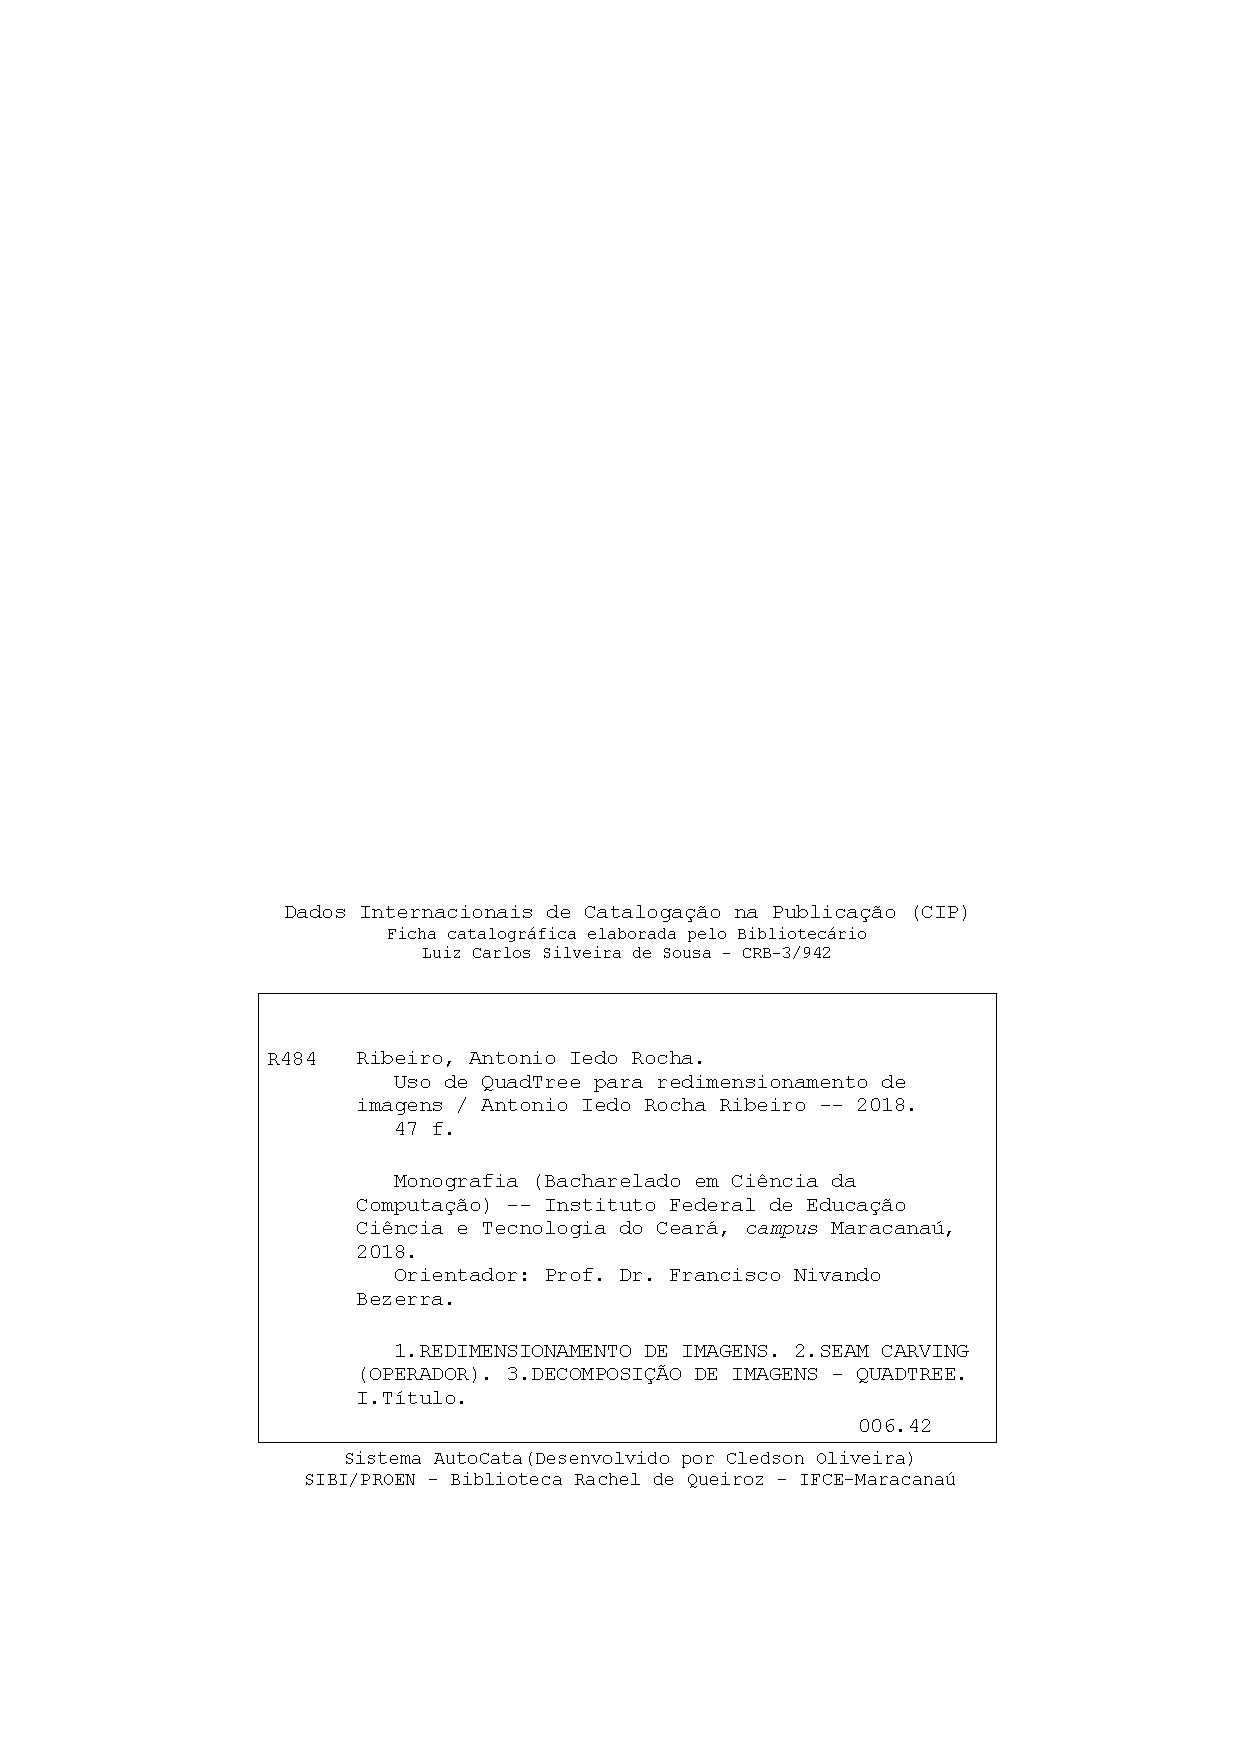
\includepdf{fichacatalografica}         % Ficha catalográfica
%\cleardoublepage

%\begin{folhadeaprovacao}
    \begin{center}
        
\includegraphics[width=2.5cm]{brasao_republica.jpg} \\
        \vspace{.5cm}
        {\ABNTEXchapterfont\large\imprimirinstituicao}
        \vspace{1cm}

        {\ABNTEXchapterfont\large\imprimirautor}

        % \vspace*{\fill}\vspace*{\fill}
        % \begin{center}
        %   \ABNTEXchapterfont\bfseries\Large\imprimirtitulo
        % \end{center}
        %\vspace*{\fill}

        %\hspace{.45\textwidth}
        % \begin{minipage}{.5\textwidth}
        %     \imprimirpreambulo
        %     {\large\imprimirdata}
        % \end{minipage}%
        %\vspace*{\fill}
    \end{center}

    \noindent Esta monografia foi julgada adequada para a obtenção do título de Bacharel em Ciência da Computação, sendo aprovada pela Coordenadoria de Telemática e pela Coordenadoria do curso de Bacharelado em Ciência da Computação do campus Maracanaú do Instituto Federal de Educação, Ciência e Tecnologia do Ceará e pela banca examinadora:

    \vfill

    \begin{center}
        % \begin{minipage}{15cm}
            \assinatura{\textbf{\imprimirorientadorRotulo~\imprimirorientador} \\ Instituto Federal de Educação, Ciência e Tecnologia do Ceará (IFCE)}

            \if \imprimircoorientador
            \else
            \assinatura{\textbf{\imprimircoorientadorRotulo~\imprimircoorientador} \\ Instituto Federal de Educação, Ciência e Tecnologia do Ceará (IFCE)}
            \fi

            \if \nomeprofessorA \instituicaoprofessorA
            \else
            \assinatura{\textbf{\imprimirnomeprofessorA}  \\ \imprimirinstituicaoprofessorA}
            \fi

            \if \nomeprofessorB
            \else
            \assinatura{\textbf{\imprimirnomeprofessorB}  \\ \imprimirinstituicaoprofessorB}
            \fi

            % \if \nomeprofessorC
            % \else
            % \assinatura{\textbf{\imprimirnomeprofessorC}  \\ \imprimirinstituicaoprofessorC}
            % \fi
        % \end{minipage}
    \end{center} 

    \vfill
    %\assinatura{\textbf{Professor}  \\ Instituto Federal do Ceará (IFCE)}

    \begin{center}
        \vspace*{\fill}
        {\large\imprimirlocal}
        \par
        {\large\imprimirdata}
        \vspace*{1cm}
    \end{center}
\end{folhadeaprovacao} 	% Folha de aprovação (Depois da apresentação)
\begin{dedicatoria}
   \vspace*{\fill}
   \centering
   \noindent
   \textit{Aos meus pais.}
   \vspace*{\fill}
\end{dedicatoria} 		    % Dedicatória
\begin{agradecimentos}
Um curso de graduação permite que o aluno seja exposto à uma grande variedade de assuntos. Tive a felicidade de encontrar um tema com o qual me identificasse ao fim do segundo ano de faculdade. Sempre tive um fascínio (de observador) pela área de Inteligência Artificial. A primeira oportunidade de trabalhar nessa área veio em meados de 2016, sob orientação do professor Ajalmar. Desde então, outras oportunidades surgiram.

Agradeço ao professor Ajalmar por me acolher como seu aluno e orientando, sugerir o tema desta monografia como trabalho de conclusão de curso e me orientar durante todos os meses de trabalho. Agradeço ainda pelos conselhos e experiências compartilhados comigo, que me permitiram dar os passos iniciais como pesquisador da área.

A universidade nos permite contato com pessoas de diferentes crenças, costumes e pensamentos. Pessoalmente, acredito que essa seja sua maior virtude. Sem dúvidas, as amizades que fiz durante toda a graduação me ajudaram a concluir este momento da minha vida. Agradeço a todos estes, desde colegas de turma aos amigos que fiz no Laboratório de Visão Computacional e Inteligência Artificial (LabVicia). Dentre todos, quero destacar três grandes amigos que fiz: Davi, que chegou a ser cofundador de uma tentativa de \textit{startup}; Victor, que hoje trabalha comigo e que em muitos momentos foi integrante de equipe nos trabalhos da faculdade; e Iedo, com o qual compartilho (atualmente) uma amizade de mais de uma década.

O processo de escrita de uma monografia é conturbado e diferente de qualquer outro trabalho mais ``comum'' da faculdade. Para encarar as dificuldades e momentos de tristeza/ansiedade, precisamos recorrer e buscar apoio naqueles que nos amam. Agradeço à minha mãe, por ser mãe. Dito isso, pode-se deduzir que esta mulher fez (e faz) de tudo por mim, desde me dar amor e carinho à me fornecer alimento e moradia; acima de tudo, me ensinando a ser uma pessoa respeitosa e responsável. Agradeço à meu pai, que mesmo à distância, sempre esteve próximo de mim, apoiando, incentivando e dando um dos melhores exemplos que posso ter de trabalho duro, caráter e responsabilidade. Agradeço ainda à meu padrasto, que assim como meu pai, sempre me mostrou a importância do trabalho e por ser um companheiro que ama e cuida de minha mãe; o fruto desse amor é o meu irmão, que traz alegria à todos em nossa família, assim como as irmãs que tenho por parte de pai. Destes, faço um último agradecimento à minha madrasta, por ter sido (e ser) uma parte essencial da minha vida.

Neste momento, gostaria de agradecer a pessoa que acompanhou todo o percurso que trilhei neste trabalho: Hannah. Uma das melhores pessoas que conheço e que me apoiou em todos os momentos de dificuldades, celebrando também as vitórias que tive. À você, palavra alguma vai expressar com precisão o que sinto por ti e o quanto sou grato por ter você em minha vida.

Agradeço também aos professores que tive durante toda minha vida, especialmente a partir do ensino médio (até onde minha memória permite-me lembrar) chegando aos da faculdade. Agradeço pelo empenho em ensinar as ferramentas necessárias na formação acadêmica, mas acima disso, pelos ensinamentos sobre a vida, respeito com o próximo e pensamento crítico. Também agradeço aos servidores do IFCE, por manterem a instituição funcionando, sempre com zelo pelo bem público.

Por fim, agradeço à você, leitor, pelo interesse neste trabalho.
\end{agradecimentos} 		% Agradecimentos
\begin{epigrafe}
    \vspace*{\fill}
	\begin{flushright}
		\textit{
            ``É necessário sempre acreditar que um sonho é possível''\\ % ``<Citação Célebre>''\\
		    (Racionais MC's) % (<Autor da citação>)
		}
	\end{flushright}
\end{epigrafe} 			% Epígrafe
\setlength{\absparsep}{18pt} % ajusta o espaçamento dos parágrafos do resumo
\begin{resumo}
    Modelos de regressão são procedimentos estatísticos que permitem estimar as relações entre as variáveis que modelam um determinado problema. É comum dividir essas relações em duas categorias: lineares e não-lineares. Quando deseja-se solucionar um problema utilizando o arcabouço de Aprendizado de Máquina (AM), é comum observar uma preferência pelo uso de modelos que estimem relações lineares. As motivações subjacentes encontram-se em formulações matemáticas mais simples que gozam de propriedades bastante conhecidas e, ademais, resultam muitas vezes em soluções analíticas. Contudo, a notória desvantagem no uso de modelos lineares é a falta de poder de generalização para problemas de cunho real; isso ocorre devido à forte natureza não-linear de diversos eventos que ocorrem no dia-a-dia. Para escapar à necessidade de criação de modelos não-lineares (que possuem uma complexidade intrínseca maior que à de modelos lineares), o uso de uma estratégia conhecida como truque do \textit{kernel} tornou-se bastante popular. Sua ideia base consiste em transformar o espaço original do problema em um espaço de Hilbert de alta -- ou infinita -- dimensão, onde os padrões apresentem comportamento linear; sendo possível, então, o uso de métodos lineares como \textit{ridge regression} para descoberta das relações entre as variáveis. A escolha de uma função que realize esta transformação espacial (chamada função de \textit{kernel}) é extremamente dependente do problema em mãos, o que levou vários pesquisadores a utilizarem funções já consolidadas, tais como \textit{rbf} e polinomial (com otimização de seus parâmetros). Porém, essa abordagem resulta em variações no desempenho para diferentes conjuntos de dados. Criar funções de \textit{kernel} que se adaptem a um determinado problema é uma solução mais conveniente, mas que gera uma carga de trabalho grande, uma vez que é necessário conhecer detalhes do problema. Nesta monografia é apresentada uma proposta baseada em Programação Genética (PG), denominada \textit{Genetic Kernels for Regression} (GKR), que propõe um método de criação automática de novas funções de \textit{kernel} adaptáveis para problemas de regressão. O método utiliza operadores de fechamento, que combinam funções de \textit{kernel} existentes para criação de novos \textit{kernels} válidos. Cada função é uma árvore sintática, onde cada nó possui um conjunto de restrições que garante a validade do \textit{kernel} criado. O modelo proposto tem seu desempenho comparado com modelos estado-da-arte, tais como \textit{Support Vector Regression} (SVR) com \textit{kernels} linear, \textit{rbf} e polinomial, e Redes Neurais Artificiais (RNA) dos tipos \textit{Multilayer Perceptron} (MLP) e \textit{Radial Basis Functions} (RBF). Os resultados permitem inferir que: (\textit{i}) o modelo proposto é bastante robusto quando apresentado a diferentes conjuntos de dados; (\textit{ii}) possui desempenho similar ao dos modelos SVR, MLP e RBF, chegando à uma leve superioridade para a maioria dos problemas utilizados nos experimentos.
    
    \textbf{Palavras-chave}: funções de \textit{kernel}, problemas de regressão, programação genética, \textit{ridge regression}, truque do \textit{kernel}.
\end{resumo} 				% Resumo em portuguê`s
\begin{resumo}[Abstract]
 \begin{otherlanguage*}{english}
   This is the english abstract.

   \vspace{\onelineskip}
 
   \noindent 
   \textbf{Keywords}: latex. abntex. text editoration.
 \end{otherlanguage*}
\end{resumo} 			% Resumo em inglês
% ---
\pdfbookmark[0]{\listfigurename}{lof}   % Lista de ilustrações
\listoffigures*
\cleardoublepage
% ---
\pdfbookmark[0]{\listtablename}{lot}    % Lista de tabelas
\listoftables*
\cleardoublepage
% ---
% \pdfbookmark[0]{\listalgorithmname}{loa}% Lista de algoritmos
% \listofalgorithms
% \cleardoublepage
% ---
% \renewcommand{\listtheoremname}{Lista de definições}
% \pdfbookmark[0]{\listtheoremname}{lod}  % Lista de definições
% \begin{KeepFromToc}
% \listoftheorems[ignoreall,show=definition]
% \end{KeepFromToc}
% \cleardoublepage
% ---
% \renewcommand{\listtheoremname}{Lista de proposições}
% \pdfbookmark[0]{\listtheoremname}{loat}  % Lista de proposições
% \begin{KeepFromToc}
% \listoftheorems[ignoreall,show={proposition}]
% \end{KeepFromToc}
% \cleardoublepage
% ---
% \renewcommand{\listtheoremname}{Lista de teoremas}
% \pdfbookmark[0]{\listtheoremname}{loat}  % Lista de teoremas
% \begin{KeepFromToc}
% \listoftheorems[ignoreall,show={theorem}]
% \end{KeepFromToc}
% \cleardoublepage
% ---
\begin{siglas}
  \item[AG] Algoritmos Genéticos
  \item[AM] Aprendizado de Máquina
  \item[CE] Computação Evolucionária
  \item[EA] \textit{Evolutionary Algorithms}
  \item[GP] \textit{Gaussian Processes}
  \item[GKR] \textit{Genetic Kernels for Regression}
  \item[IA] Inteligência Artificial
  \item[KRR] \textit{Kernel Ridge Regression}
  \item[LSSVR] \textit{Least Squares Support Vector Regression}
  \item[ML] \textit{Machine Learning}
  \item[MLP] \textit{Multilayer Perceptron}
  \item[MOGP] \textit{Multi-Objective Genetic Programmming}
  \item[PG] Programação Genética
  \item[PSO] \textit{Particle Swarm Optimization}
  \item[RBF] \textit{Radial Basis Function}
  \item[RKHS] \textit{Reproducing Kernel Hilbert Spaces}
  \item[RNA] Redes Neurais Artificiais
  \item[RMSE] \textit{Root Mean Square Error}
  \item[STGP] \textit{Strongly-Typed Genetic Programming}
  \item[SVM] \textit{Support Vector Machine}
  \item[SVR] \textit{Support Vector Regression}
\end{siglas}  	    % Lista de abreviaturas e siglas
\begin{simbolos}
    \item[$\lVert.\rVert$] Norma euclidiana
    \item[$\boldsymbol{\alpha}$] Vetor de coeficientes de Lagrange
    \item[$d$] Grau do polinômio
    \item[$\mathcal{D}$] Conjunto de dados
    \item[$\epsilon$] Erro
    \item[$\boldsymbol{\epsilon}$] Vetor de erros
    \item[$f(.)$] Função
    \item[$\mathcal{H}$] Espaço de Hilbert
    \item[$\mathbf{I}_n$] Matriz Identidade ($n \times n$)
    \item[$\kappa(.,.)$] Função de \textit{kernel}
    \item[$K$] Matriz de \textit{kernel}
    \item[$L$] Função Lagrangiana
    \item[$\mathcal{L}$] Função de perda quadrática
    \item[$\lambda$] Fator de regularização
    \item[$n$] Número de padrões de um conjunto de dados
    \item[$\mathcal{O}$] Custo assintótico
    \item[$p$] Dimensão de um padrão
    \item[$\phi(.)$] Função de mapeamento
    \item[$\sigma$] Abertura da gaussiana
    \item[$\mathbb{R}$] Conjunto dos números Reais
    \item[$\mathbf{x}$] Padrão, amostra ou instância
    \item[$y$] Rótulo de um padrão
    \item[$\mathbf{w}$] Vetor de coeficientes de regressão
    \item[$\mathbf{\hat{w}}$] Vetor ótimo de coeficientes de regressão
\end{simbolos} 	    	    % Lista de símbolos
% ---
\pdfbookmark[0]{\contentsname}{toc}     % Sumário
\tableofcontents*
\cleardoublepage
% ---

% ----------------------------------------------------------
% ELEMENTOS TEXTUAIS
% ----------------------------------------------------------
\textual

% ---------
% Capítulos
% ---------
\chapter{Introdução} \label{chapter:introduction}
% O conceito de ensinar uma máquina, ou um conjunto delas, a realizar tarefas que requerem a capacidade do pensamento humano e raciocínio data da antiguidade. Na Ilíada de Homero \cite{homero2015}, o deus Hefesto, considerado deus da tecnologia, cria máquinas humanoides de bronze com o objetivo de auxiliá-lo a se movimentar. Entretanto, a criação da inteligência artificial (IA) nos moldes atuais é atribuída a Alan Turing, quando o mesmo propôs o conhecido ``teste de Turing'' como uma medida da inteligência de máquina.

% A inteligência humana tem despertado curiosidade há mais de dois milênios.   O campo de inteligência artificial (IA) nasce a partir de uma combinação de diferentes ideias provenientes de trabalhos, em grande maioria, destas áreas. 
% O processo de aprendizagem humano é tão complexo que definir o termo aprendizagem torna-se difícil.
% Desde o surgimento dos computadores houveram especulações acerca da possibilidade de ensiná-los a realizar tarefas inteligentes.
% A inteligência é um termo complexo e definí-lo precisamente mostra-se um trabalho árduo. Mais especificamente,
% A competência que o ser humano demonstra na realização de atividades como reconhecimento de objetos e comunicação via elaborados sistemas de linguagens sempre
% O estudo sobre aprendizagem e inteligência é uma das disciplinas mais antigas
% A competência que o ser humano apresenta na realização de atividades como reconhecimento de objetos e comunicação via elaborados sistemas de linguagens o difere dos demais seres vivos.
% O ser humano, graças à sua capacidade mental, possui habilidades únicas que o difere dos demais seres vivos.
% Reconhecimento visual de objetos, comunicação via elaborados sistemas de linguagens e extrema competência em disciplinas científicas são alguns exemplos que mostram o potencial de aprendizagem e evolução.
% A capacidade de aprender, em linhas gerais, é um objeto de
% A capacidade de aprender do ser humano é um objeto de estudo que desperta interesse e intriga pesquisadores de diversas áreas de pesquisa, como filosofia, psicologia, neurociência etc. Aprendizagem, assim como inteligência, abrange um vasto conjunto de processos interoperantes de uma maneira tão complexa que torna difícil de ser definida. Habilidades singulares, tais como reconhecimento visual de objetos, comunicação via elaborados sistemas de linguagens e a criação de complexos teoremas nas mais difíceis disciplinas, são apenas alguns exemplos que mostram como o constante processo de aprendizado torna nossa espécie tão única.
% Por centenas de anos, muito foi estudado acerca de como o processo de aprendizagem do cérebro humano funciona. Entretanto, a inteligência artificial (ou IA) busca não somente entender como funciona, mas também construir entidades que tenham habilidade de aprender \cite{Russell:2009:AIM:1671238}.

As capacidades cognitivas características do ser humano despertam interesse e curiosidade há séculos. O modo como percebemos, entendemos e manipulamos o mundo à nossa volta tem nos destacado dos demais seres vivos, de modo a nos classificar como seres racionais. A busca pelo conhecimento acerca de nossas tomadas de decisões (inteligentes) abrange áreas de estudo tais como filosofia, matemática, psicologia e fisiologia. De fato, uma mescla dessas áreas decorreu na criação do campo de Inteligência Artificial (IA). Entretanto, o objetivo da IA transcende aos de seus gestores pois esforça-se não somente em entender entidades inteligentes, como também construí-las \cite{russell2009}.

Apesar de não haver concordância sobre a definição universal do termo ``inteligência'', pode-se encontrar muitas similaridades entre as diversas existentes, tais como a recorrência dos termos conhecimento e aprendizado. Com o intuito de criar entidades inteligentes, muitos paradigmas de aprendizado foram propostos à medida que as pesquisas em IA foram amadurecendo. Um dos principais é o aprendizado indutivo, um processo de aquisição de conhecimento através da extração de inferências indutivas fornecidas por um professor/instrutor ou ambiente externo.

Ao aperfeiçoamento do desempenho de um agente inteligente na realização de uma determinada tarefa por meio da experiência é dado o nome de Aprendizado de Máquina (AM) \cite{mitchell1997}. Mais particularmente, o processo que induz um agente inteligente a aprender como realizar com êxito determinada tarefa se dá através da existência de exemplos na forma (\textit{entrada}, \textit{saída}). Esses exemplos são utilizados no estágio de treinamento do agente, onde este aprende relações e/ou características intrínsecas -- e de difícil detecção por humanos -- do problema a ser solucionado.

A área de AM compreende duas grandes subáreas, cada qual com seus objetivos e modelos específicos, a saber: aprendizado supervisionado e aprendizado não-supervisionado. Em aprendizado supervisionado, o objetivo é predizer uma relação funcional entre as características dos objetos de estudo e seus rótulos. No sentido mais específico, se os rótulos possuem valores discretos, a tarefa compreende solucionar problemas de classificação; quando os rótulos possuem valores contínuos, a tarefa lida com problemas de regressão, ou aproximação de funções. Aprendizado não-supervisionado tem como objetivo descrever um conjunto de objetos de estudo, usualmente através de medidas de similaridade/dissimilaridade. Diferente do aprendizado supervisionado, neste não há informação dos rótulos dos objetos. Em grande parte, as tarefas desta subárea focam em agrupamento, sumarização e associação dos objetos utilizados no treinamento \cite{gama2011}. A Figura \ref{fig:ch1-1} apresenta um resumo da hierarquia de AM.

\begin{figure}[H]
    \caption{Hierarquia de aprendizado.}
    \label{fig:ch1-1}
    \def\gap{13mm}
    \centering
    \begin{tikzpicture}[->, >=stealth', auto, level distance=2cm,
        every node/.style = {shape=rectangle, rounded corners,
        draw, align=center, fill=blue!20, text=blue, minimum height=2em},
        root/.style = { text width=(\textwidth-6*\gap)/2 },
        level 1/.style = { sibling distance=8cm },
        level 2/.style = { sibling distance=3cm }]
    
        \node [root] {\scriptsize Aprendizado de Máquina}
        child { node {\scriptsize Supervisionado}
            child { node {\scriptsize Classificação} }
            child { node {\scriptsize Regressão} }
        }
        child { node {\scriptsize Não-Supervisionado}
            child { node {\scriptsize Agrupamento} }
            child { node {\scriptsize Associação} }
            child { node {\scriptsize Sumarização} }
        };
    \end{tikzpicture}
    \begin{center}
        \makebox[\width]{Fonte: \citeonline{gama2011}.}
    \end{center}
\end{figure}

O foco desta monografia reside em aprendizado supervisionado, e mais particularmente em problemas de regressão.

\section{Motivação}

Uma tarefa de regressão pode ser descrita como um processo estatístico onde procura-se estimar a relação entre as variáveis independentes e dependentes de uma função-objetivo. Essa relação pode ser tanto linear como não-linear. Em AM, há uma preferência por modelos que descrevem relações lineares por estes possuírem tanto uma formulação matemática mais simples quanto propriedades analíticas bem conhecidas. Contudo, modelos lineares têm uma grande desvantagem: como grande parte dos problemas do mundo real possui natureza não-linear, é extremamente complicado -- muitas vezes, impossível -- modelá-los através de relações lineares. A Figura \ref{fig:ch1-linear} exemplifica bem essa dificuldade, onde uma regressão linear simples tenta ajustar sua superfície (uma reta) a dados gerados por uma função polinomial.

Apesar de sua popularidade, métodos de regressão linear não permitem a solução de grande parte de problemas do mundo real. Portanto, surge a necessidade da utilização de modelos não-lineares para descrever relações de dependência que permitam predições bem-sucedidas \cite{hofmann2008}.

A criação de modelos não-lineares figura como uma tarefa laboriosa e exige que o(a) projetista demande muito tempo de trabalho em sua concepção. Felizmente, uma alternativa à este processo, conhecida como truque do \textit{kernel}, tornou-se bastante popular nos últimos anos. Este consiste em transformar o espaço original do problema para um espaço de maior (às vezes, infinita) dimensão, onde os dados apresentam comportamento linear. Uma vez neste novo espaço, métodos lineares podem ser utilizados para encontrar as relações entre as variáveis do problema.

\begin{figure}[ht]
    \centering
    \caption{Resultado da predição obtida por uma regressão linear simples sobre dados gerados por uma função polinomial.}
    \label{fig:ch1-linear}
    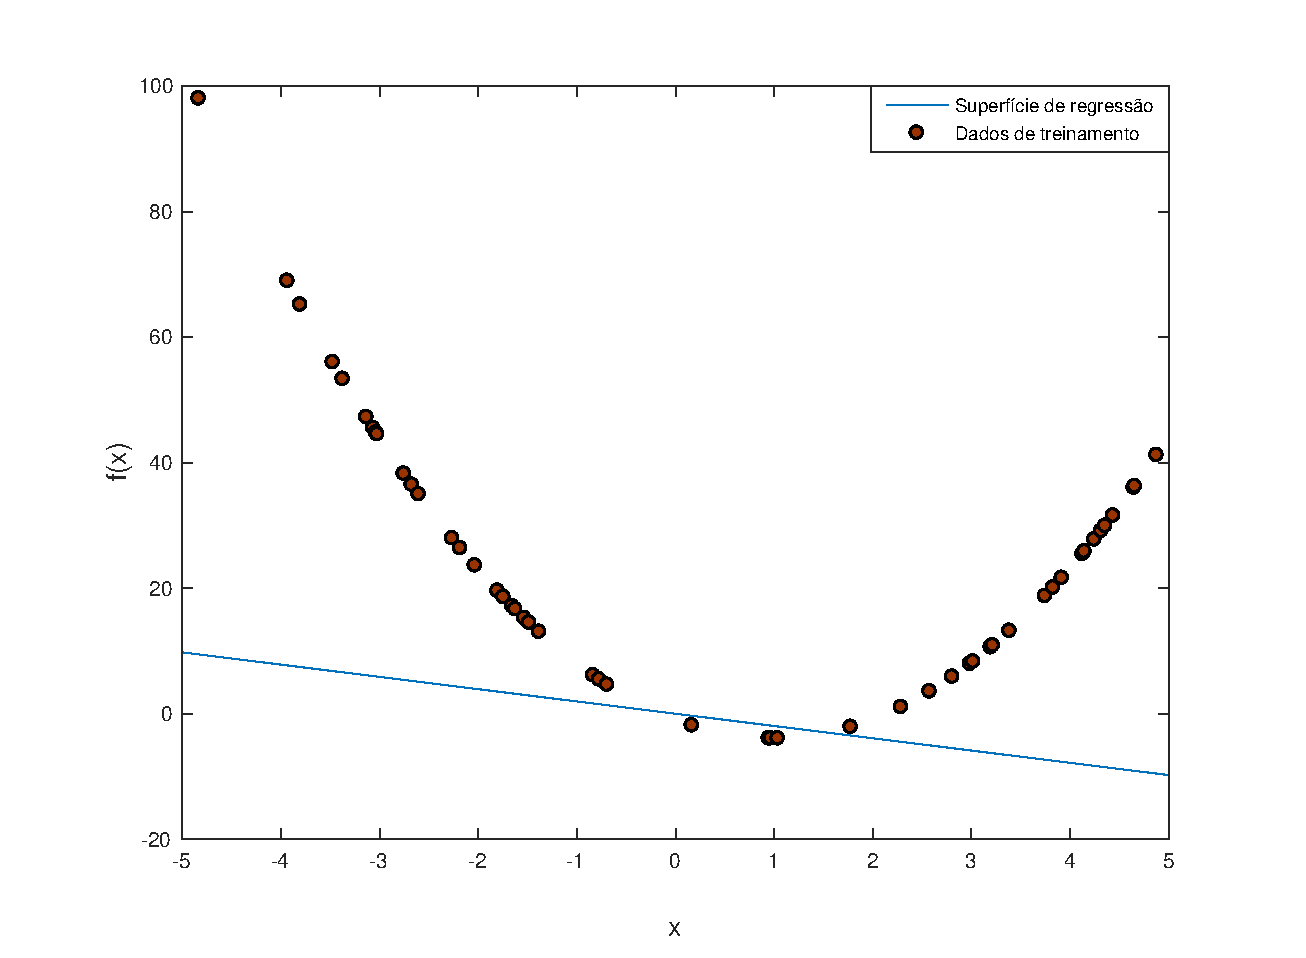
\includegraphics[width=.5\linewidth]{chapter1/linear.eps}
    \begin{center}
        \makebox[\width]{Fonte: Autor.}
    \end{center}
\end{figure}

O truque do \textit{kernel} pode ser visto como um atalho computacional que traz duas grandes vantagens: (\textit{i}) permite a criação de extensões (não-lineares) de métodos lineares; e (\textit{ii}) não exige demasiados recursos computacionais, pois não é necessário o cômputo do mapeamento de forma explícita. Não à toa, esses métodos tornaram-se tão populares em problemas de regressão \cite{shawe2004}. A Figura \ref{fig:ch1-poly} exemplifica bem o poder do truque do \textit{kernel}, onde predições mais precisas são realizadas ao utilizar uma mapeamento dos dados com uma função polinomial, e aplicando o método KRR. Mais informações sobre KRR e o truque do \textit{kernel} podem ser obtidas no Capítulo \ref{chapter:kernel-methods}.

\begin{figure}[H]
    \centering
    \caption{Resultado da predição obtida pelo modelo KRR com uma função de mapeamento polinomial.}
    \label{fig:ch1-poly}
    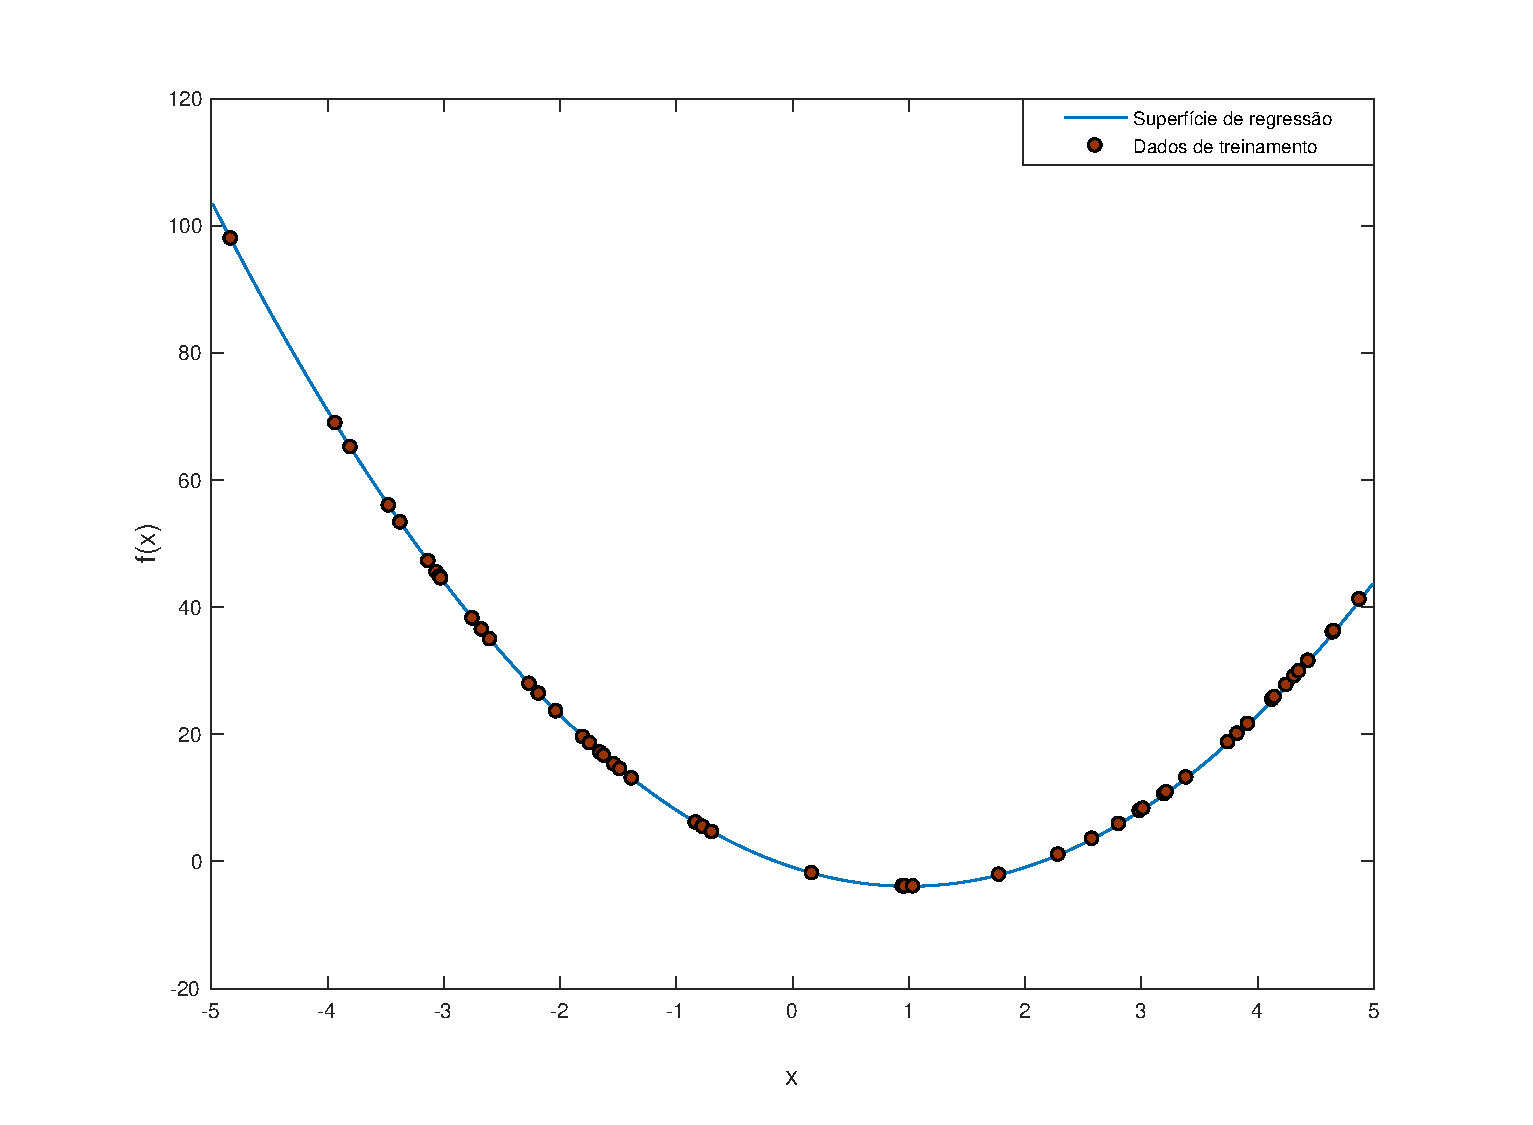
\includegraphics[width=.5\linewidth]{chapter1/poly.eps}
    \begin{center}
        \makebox[\width]{Fonte: Autor.}
    \end{center}
\end{figure}

\clearpage

Deste modo, em tarefas de regressão baseada em métodos de \textit{kernel}, o objetivo é encontrar uma função que mapeie os dados originalmente não-lineares, para um espaço onde estes apresentem-se linearmente \cite{smola1998}. Encontrar tal função é uma tarefa árdua, tanto que muitos pesquisadores optam por utilizar \textit{kernels} clássicos, tais como \textit{rbf} e polinomial, otimizando apenas seus parâmetros. Contudo, essa abordagem resulta em variações no desempenho para diferentes conjuntos de dados \cite{howley2005}. Criar funções de \textit{kernel} que se adaptem a um determinado conjunto de dados é uma solução mais conveniente e tornou-se um tópico de muito interesse da comunidade acadêmica, sendo chamado também de ``tópico quente'' (do inglês, \textit{hot topic}).

% \section{Trabalhos relacionados} \label{sec:related-work}
Técnicas de Computação Evolucionária (CE), como Programação Genética (PG), têm sido bastante utilizadas na criação automática de novas funções de \textit{kernel} em diferentes classes de problemas. Entretanto, na maioria destes estudos, técnicas de PG são aplicadas em tarefas de classificação utilizando Máquinas de Vetores Suporte (\textit{Support Vector Machines}, SVM). O primeiro trabalho que se tem registro da utilização de PG para criação de novos \textit{kernels} foi proposto por \citeonline{howley2005}. Neste, os autores utilizam a evolução em paralelo de cinco populações (de \textit{kernels}) com o objetivo de eliminar o teste de várias combinações de parâmetros. Ao fim do processo, o indivíduo mais apto de todas as populações é escolhido como o \textit{kernel} utilizado na criação do modelo final.

Em \cite{howley2006}, os autores reconhecem a capacidade de criação automática de novos \textit{kernels} e focam seu uso especificamente para classificadores SVM. As diferenças primordiais entre esta proposta e a anterior encontram-se em uma representação mais sofisticada do \textit{kernel}, função de aptidão baseada em validação cruzada e um filtro de Mercer (se um \textit{kernel} não obedece ao teorema, recebe o valor mais baixo de aptidão).

\citeonline{diosan2007} utilizam um conjunto de operadores maior que \cite{howley2006}, incluindo operadores que transformam o espaço $\mathbb{R}^p$ no espaço $\mathbb{R}$. Entretanto, os autores não garantem que os \textit{kernels} criados obedeçam ao teorema de Mercer. Apesar disso, os resultados obtidos são bons e possuem um desempenho ligeiramente superior aos \textit{kernels} clássicos.

\citeonline{sullivan2007} utilizam uma técnica de PG conhecida como \textit{Strongly-Typed Genetic Programming} (STGP) para garantir que cada nó da árvore possa ter somente um determinado conjunto de operadores e/ou terminais como candidatos a nós-filho. Essa técnica permite que o \textit{kernel} gerado obedeça ao teorema de Mercer.

\citeonline{girdea2007} utilizam apenas combinações dos kernels linear, \textit{rbf} e polinomial na construção de novos \textit{kernels}. Além disso, o fator que o diferencia dos demais trabalhos é o uso de um meta-algoritmo conhecido como \textit{boosting}, que tem como objetivo combinar os resultados de classificadores mais ``fracos'' para formar um classificador mais preciso. Em particular, é utilizado o algoritmo InfoBoost \cite{aslam2000}.

\citeonline{alizadeh2011} apresentam uma abordagem diferente das anteriores. Os \textit{kernels} construídos durante o processo evolutivo são utilizados como entradas dos \textit{kernels} linear e \textit{rbf}. A partir destes, a classificação é efetuada. Os resultados confirmam uma superioridade de desempenho sobre os \textit{kernels} clássicos. Contudo, para conjuntos de dados de alta dimensão, o espaço de busca pelo \textit{kernel} ideal torna-se inviável. Os autores propõem mapear os dados de entrada para espaços de menor dimensão que o original, porém com mais de uma dimensão. Tal proposta não foi investigada e, assim, o trabalho dos autores não alcança o desempenho almejado (se comparado aos trabalhos anteriores).

Outro trabalho interessante que aplica PG para combinação de \textit{kernels} foi proposto por \citeonline{schuh2012}, que utilizam Enxame de Partículas (\textit{Particle Swarm Optimization}, PSO) como fator adicional no processo de evolução. A combinação de \textit{kernels} é também aplicada em problemas específicos, como classificação de imagens \cite{ribeiro2015}, classificação de sequências de DNA hipersensíveis \cite{kamath2011} e classificação de padrões em expressão de genes \cite{cuong2006}.

Enquanto os trabalhos descritos nos parágrafos anteriores focam suas aplicações para tarefas de classificação (genéricas e específicas), não foram encontradas aplicações em problemas de regressão. Dessa forma, este trabalho propõe a criação de novas funções de \textit{kernel} a partir de outras preexistentes aplicadas em problemas de regressão, visto ser uma área pouco explorada. Para alcançar esse objetivo, é utilizado PG para combinação das funções de \textit{kernel} de base. Através do uso de propriedades de construção de novos \textit{kernels}, em conjunto com uma representação genética de STGP podemos garantir que as funções geradas obedecem ao teorema de Mercer. Para fins de avaliação, a proposta é comparada a métodos estado-da-arte, tais como Regressão de Vetores Suporte (\textit{Support Vector Regression}, SVR) e Redes Neurais Artificiais (RNA) do tipo Perceptron Multicamadas (\textit{Multilayer Perceptron}, MLP) e Funções de Base Radial (\textit{Radial Basis Functions}, RBF).

\section{Objetivos Geral e Específicos}
Este trabalho tem como objetivo geral propor um método de criação automática de novas funções de \textit{kernel} adaptáveis para problemas de regressão. Para alcançar esse objetivo deve-se utilizar PG para criar combinações de funções já conhecidas. Através dessas combinações, o método garante adaptabilidade ao criar \textit{kernels} específicos para cada problema.

Mais particularmente, este trabalho possui os seguintes objetivos específicos:

\begin{itemize}
	\item Avaliar o desempenho do modelo proposto em realizar predições para problemas de regressão, assim como seu tempo médio de execução.
    \item Avaliar o uso de um determinado conjunto de funções de \textit{kernel} como base do processo de combinação e evolução, para criação de novos \textit{kernels}.
    \item Criar um mecanismo de geração automática de funções de \textit{kernel} que melhor se adaptem a um determinado problema.
    \item Comparar o desempenho do modelo proposto com o de modelos estado-da-arte, como SVR e Redes Neurais Artificiais.
    \item Verificar e validar a aplicação da \textit{ridge regression} no espaço de características gerado pelas funções de \textit{kernels} criadas.
\end{itemize}

\section{Estrutura da Monografia}
Esta monografia é composta de cinco capítulos -- além deste --, organizados da seguinte forma: fundamentos de programação genética; métodos de \textit{kernel} para regressão, incluindo o modelo proposto; simulações computacionais; conclusões e trabalhos futuros.

De modo geral, os Capítulos \ref{chapter:genetic-programming} e \ref{chapter:kernel-methods} apresentam os fundamentos teóricos necessários para o entendimento deste trabalho. No Capítulo \ref{chapter:genetic-programming} são descritos os principais conceitos sobre o arcabouço de PG. O nível de detalhes, uso de figuras para exemplificação ajudarão na definição do modelo GKR. O Capítulo \ref{chapter:kernel-methods} apresenta o conceito de regressão linear e o uso dos mínimos quadrados para estimação dos coeficientes de regressão. Apresenta ainda uma versão mais genérica da regressão linear, chamada de \textit{ridge regression}, que realiza um balanceamento entre a norma e o erro. A última seção de fundamentos teóricos deste capítulo apresenta a formulação dual e como a partir desta, surge naturalmente a ideia de funções de \textit{kernel}. Na última seção do Capítulo \ref{chapter:kernel-methods} é apresentada a proposta deste trabalho, denominada \textit{Genetic Kernels for Regression} (GKR).

No Capítulo \ref{chapter:simulations} são apresentadas a metodologia utilizada, as simulações computacionais e os resultados obtidos, além das respectivas discussões. São utilizados problemas de natureza artificial e real. Os problemas de natureza artificial auxiliam na prova de conceito acerca do funcionamento do modelo proposto, enquanto os problemas de natureza real auxiliam na análise de desempenho do modelo em solucionar problemas do mundo real. São apresentadas tabelas com o RMSE e tempo totais (treinamento e teste) médios, assim como gráficos dos valores de aptidão médios ao longo das gerações.

O Capítulo \ref{chapter:conclusions} apresenta as conclusões e considerações finais sobre este trabalho. Por fim, é apresentada uma proposta de trabalho futuro.
\chapter{Programação Genética} \label{chapter:genetic-programming}
O desejo pela existência de máquinas que possam solucionar problemas de forma automática (ou seja, sem a interferência de um ser humano) é tema central e um dos principais objetivos da área de AM. \citeonline{samuel1983}, um dos pioneiros da área, afirmou que o objetivo do aprendizado de máquinas ``é fazer com que máquinas tenham comportamento, que se feito por humanos, seria assumido haver o uso de inteligência''.

Programação Genética (PG) é uma técnica de Computação Evolucionária (CE) que evolui programas de computador a fim de resolver problemas de forma automática sem que seja necessário conhecer, \textit{a priori}, a estrutura ou detalhes do problema. Em um nível maior de abstração, PG é um método sistemático, independente de domínio, utilizado para fazer computadores solucionarem problemas automaticamente partindo de uma declaração de alto nível do que precisa ser feito \cite{poli2008}.

Assim como outras técnicas evolucionárias\footnote{Estas são também chamadas de algoritmos evolucionários (\textit{evolutionary algorithms}, EA).}, PG segue o princípio \textit{darwiniano} -- comumente chamado de ``sobrevivência do mais apto''. De acordo com esse princípio, os indivíduos que se adaptarem melhor ao ambiente em que vivem, têm mais chances de sobreviver e perpetuar suas características para gerações futuras de sua espécie.

Por ser baseado nas leis da evolução natural, PG pode ser descrita como um processo estocástico, não podendo garantir que uma solução para um problema seja encontrado \cite{poli2008}. Entretanto, sua natureza aleatória a permite percorrer um espaço de busca maior e escapar de armadilhas em que métodos determinísticos são capturados. Tais características tem sido um ponto favorável à PG, que apresentou sucesso em diversos domínios de aplicações e tem sido capaz de criar programas melhores que aqueles escritos por programadores humanos \cite{banzhaf1998}.

Este capítulo discute os principais conceitos e componentes de um sistema baseado em programação genética. Primeiramente, na seção \ref{sec:overview} é dada uma visão geral acerca do algoritmo padrão da PG. A seção \ref{sec:representation} apresenta a estrutura de um indivíduo e os componentes que a formam. Métodos para criação da população inicial são discutidos na seção \ref{sec:initial-population}. A função de aptidão, que define o quão bom é um indivíduo ao solucionar o problema, é discutida na seção \ref{sec:fitness-functions}. Métodos de seleção são apresentados e analisados na seção \ref{sec:selection-methods}. A seção \ref{sec:genetic-operators} apresenta os operadores genéticos de reprodução, cruzamento e mutação. Os critérios de parada do algoritmo da PG são discutidos na seção \ref{sec:termination}. A seção \ref{sec:stgp} apresenta a versão fortemente tipada da PG. Por fim, a seção \ref{sec:bloat-growth} analisa brevemente potenciais problemas que um sistema baseado em PG pode enfrentar.

\section{Visão geral} \label{sec:overview}
Um sistema baseado em PG é responsável por evoluir uma população de indivíduos, geração a geração, em busca do indivíduo mais apto a resolver um determinado problema. Os passos básicos de um sistema baseado em PG são descritos no algoritmo \ref{alg:pg}. No início de cada geração, todos os indivíduos da população são avaliados de acordo com um critério de qualidade preestabelecido, e um valor de aptidão (do inglês, \textit{fitness}) é atribuído a cada um deles. Em seguida, um processo de seleção é realizado para escolha dos mais aptos a criarem os indivíduos da próxima população. A criação da nova população se dá através de duas operações: cruzamento e/ou mutação. O operador de cruzamento combina partes aleatórias de dois indivíduos a fim de gerar um filho. O objetivo desse operador é melhorar futuras gerações através da recombinação de bons indivíduos. Já o operador de mutação cria um novo filho alterando aleatoriamente uma parte aleatória de um dos indivíduos selecionados. Esse operador adiciona mais diversidade à população com objetivo de evitar uma convergência prematura ou a parada em mínimos locais do espaço de busca. A Figura \ref{fig:pg-workflow} apresenta uma visão de fluxograma do algoritmo descrito acima.

% Define block styles
\tikzstyle{decision} = [diamond, draw, fill=blue!20,
    text width=8em, aspect=2, text centered, node distance=3cm, inner sep=0pt]
\tikzstyle{block} = [rectangle, draw, fill=blue!20,
    text width=8em, text centered, rounded corners, minimum height=3em]
\tikzstyle{line} = [draw, -latex']

\begin{figure}[H]
    \caption{Fluxograma do algoritmo padrão de PG.}
    \label{fig:pg-workflow}
    \begin{tikzpicture}[node distance = 4cm, auto]
        % Place nodes
        \node [draw=none] (start) {};
        \node [block, node distance = 2.5cm, right of=start] (init) {\scriptsize criar população inicial};
        \node [block, node distance = 4cm, right of=init] (qualitycheck) {\scriptsize avaliação da aptidão};
        \node [decision, right of=qualitycheck, node distance=4.5cm] (decide) {\scriptsize Algum critério de parada atendido?};
        \node [block, text width=3em, right of=decide, node distance=4cm] (stop) {\scriptsize parar};
        \node [block, below of=decide, node distance=3.5cm] (selection) {\scriptsize seleção dos indivíduos};
        \node [block, left of=selection, node distance=4.5cm] (breeding) {\scriptsize Reprodução \\(cruzamento, mutação)};

        % Draw edges
        \draw[red, very thick, dotted, rounded corners] ($(breeding.north west)+(-0.8,0.8)$) rectangle ($(selection.south east)+(0.8,-0.8)$) node[text=black] at ($(breeding.south east)+(0.5,-0.5)$, 0) {\scriptsize Processo de reprodução};
        \path [line] (start) -- (init);
        \path [line] (init) -- (qualitycheck);
        \path [line] (qualitycheck) -- (decide);
        \path [line] (decide) -- node {\scriptsize sim} (stop);
        \path [line] (decide) -- node[pos=.3] {\scriptsize não} (selection);
        \path [line] (selection) -- (breeding);
        \path [line] (breeding) -- node[pos=.5] {\scriptsize Nova população} (qualitycheck);
    \end{tikzpicture}
    \begin{center}
        \makebox[\width]{Fonte: Autor.}
    \end{center}
\end{figure}

\begin{algorithm}
    \caption{Algoritmo padrão da PG}
    \label{alg:pg}
    \begin{algorithmic}[1]
        \Begin
        \State Crie uma população inicial de forma aleatória utilizando os conjuntos primitivos.
        \Repeat
        \State Execute cada programa e defina sua aptidão.
        \State Selecione um, ou dois, programa(s) da população.
        \State Crie novo(s) programa(s) através das operações genéticas.
        \Until uma solução aceitável seja encontrada ou algum critério de parada seja atendido.
        \State \Return o melhor programa encontrado.
    \End
    \end{algorithmic}
\end{algorithm}

\section{Representação} \label{sec:representation}
O primeiro estágio na concepção de uma técnica evolucionária é decidir qual a representação genética de um indivíduo \cite{eiben2015}. Esse estágio é um dos mais importantes pois influencia diretamente no projeto de operadores genéticos. Ao propor o algoritmo de PG, \citeonline{koza1992} utilizou estruturas em árvores -- também conhecidas como árvores sintáticas -- para a representação de um indivíduo. Várias outras representações foram propostas ao longo dos anos seguintes. Apesar disso, as árvores permaneceram como a representação mais utilizada em PG \cite{poli2008}.

De modo geral, árvores são uma das estruturas mais utilizadas na representação de objetos na ciência da computação. Em PG, as árvores são responsáveis por capturar expressões através do uso de uma sintaxe formal. Dependendo do problema a ser solucionado, e da percepção do projetista de como a solução deve ser, uma árvore pode representar expressões aritméticas, fórmulas em lógica de predicado de primeira ordem, ou códigos escritos em uma linguagem de programação. Para fins de exemplificação, a Figura \ref{fig:tree-example} ilustra a árvore sintática correspondente à expressão aritmética $\sin(3x) \times 3\cos(x)$.

\begin{figure}[H]
    \caption{Árvore sintática representando a expressão aritmética $\sin(3x) \times 3\cos(x)$.}
    \label{fig:tree-example}
    \begin{center}
        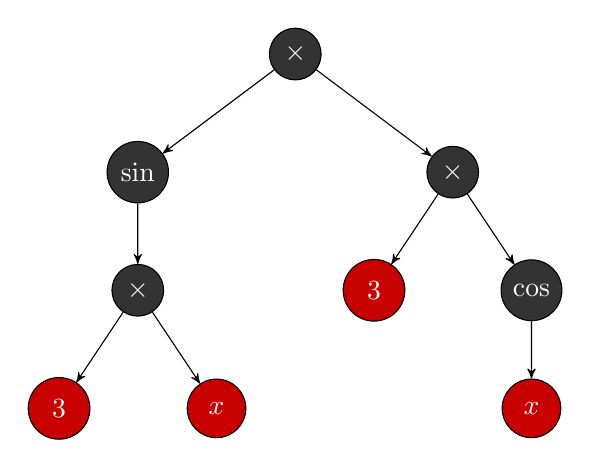
\begin{tikzpicture}[->,>=stealth',auto,
        black/.style={fill=my_black},
        red/.style={fill=my_red, inner sep=5pt},
        default/.style={draw, circle, text=white},
        level 1/.style={sibling distance=40mm},
        level 2/.style={sibling distance=20mm}]
        \node [arn_r, default, black] {$\times$}
        child{ node [arn_r, default, black] {$\sin$}
            child{ node [arn_r, default, black] {$\times$}
                child{ node [arn_r, default, red] {$3$} }
                child{ node [arn_r, default, red] {$x$} }
            }
        }
        child{ node [arn_r, default, black] {$\times$}
            child{ node [arn_r, default, red] {$3$} }
            child{ node [arn_r, default, black] {$\cos$}
                child{ node [arn_r, default, red] {$x$} }
            }
        };
        \end{tikzpicture}
    \end{center}
    \begin{center}
        \makebox[\width]{Fonte: Autor.}
    \end{center}
\end{figure}

Dessa forma, definir a forma de um indivíduo resume-se em definir a sintaxe da árvore. No contexto mais amplo da ciência da computação, os elementos que compõem uma árvore são chamados de \textbf{nós}, onde o nó mais ao topo da árvore é chamado de raiz, e os nós em níveis mais profundos são chamados de folhas. No contexto de PG, existem dois tipos de nós: (\textit{i}) terminais, que correspondem aos nós folha; (\textit{ii}) funções, que são os nós internos (incluindo a raiz da árvore). Na Figura \ref{fig:tree-example}, os nós folha são representados pela cor vermelha, enquanto os nós internos são representados pela cor cinza.

O conjunto de terminais é constituído de todas as variáveis, funções com aridade (número de argumentos) 0, e constantes utilizadas para solucionar o problema \cite{poli2008,banzhaf1998}. As constantes podem assumir valores inteiros, cadeias de caracteres, números de ponto flutuante etc.

O conjunto de funções é constituído por todas as funções específicas ao domínio do problema a ser solucionado \cite{poli2008}. Exemplos de tais funções são operadores aritméticos, lógicos, declarações condicionais e de laços. Vale ressaltar que o conjunto de funções pode conter quaisquer funções que sejam úteis no domínio do problema. Abaixo, uma lista de funções frequentemente utilizadas é apresentada, extraída de \cite{poli2008,banzhaf1998}:

\begin{itemize}
    \item Operadores aritméticos: \{ $+, -, \times, /$ \};
    \item Operadores matemáticos: \{ $\sin, \cos, \tan, \exp, square$ \};
    \item Operadores lógicos: \{ AND, OR, NOT \};
    \item Operadores condicionais: \{ If-Then-Else \}.
\end{itemize}

% \begin{itemize}
%     \item \textbf{Adaptabilidade}: contrariamente à estrutura de um indivíduo em algoritmos genéticos, que possui tamanho fixo, uma população em PG pode possuir indivíduos de diferentes formas, tamanhos e complexidade. Os termos ``tamanho'' e ``forma'' referem-se à profundidade máxima da árvore e o fator de ramificação dos nós, respectivamente.
%     \item \textbf{Gramática específica de domínio}: uma gramática deve ser definida de forma a representar de forma precisa o problema em questão A gramática deve, ainda, ser capaz de representar qualquer solução possível.
% \end{itemize}

\citeonline{koza1992} ainda define duas restrições que devem ser satisfeitas pelos conjuntos de terminais e funções (chamados de conjunto primitivos) para que o algoritmo de PG funcione apropriadamente:

\begin{enumerate}
    \item \textbf{Fechamento}: qualquer função do conjunto de funções deve ser capaz de operar com todos os valores recebidos como entrada. Dessa forma, é garantido que sejam geradas árvores sintaticamente viáveis.
    \item \textbf{Suficiência}: garante a convergência do sistema, fazendo com que os conjuntos de funções e terminais sejam capazes de representar uma solução viável para o problema a ser solucionado.
\end{enumerate}

Embora destaquem-se como a estrutura mais utilizada na representação de indivíduos em PG, o uso de árvores sintáticas possui uma implicação importante a ser mencionada: contrariamente à estrutura de um indivíduo em algoritmos genéticos (AG), que possui tamanho fixo, uma população em PG pode possuir indivíduos de diferentes formas, tamanhos e complexidade\footnote{Os termos ``tamanho'' e ``forma'' referem-se ao número de nós da árvore e o fator de ramificação dos nós, respectivamente.}. Dessa forma, são necessários métodos de criação de indivíduos que considerem essa flexibilidade. A seção \ref{sec:initial-population} apresenta os principais métodos de criação de indivíduos em PG.

\section{População inicial} \label{sec:initial-population}
O passo seguinte à escolha de uma estrutura adequada para a representação de um indivíduo é criar a população inicial, comumente chamada de geração zero. Como em qualquer outra técnica evolucionária, os indivíduos da população inicial são tipicamente criados de modo aleatório \cite{poli2008,banzhaf1998}. Existem várias abordagens para a criação de indivíduos. A seguir são apresentados os três métodos mais utilizados para criação da população inicial, a saber: \textit{full}, \textit{grow} e \textit{ramped half-and-half}. Métodos adicionais para criação da população inicial (com indivíduos em forma de árvores) são examinados e descritos por \citeonline{luke2001}.

Três pontos devem ser mencionados antes da apresentação dos métodos. O primeiro é a definição do termo profundidade. A profundidade de um nó é a distância a partir do nó raiz para este determinado nó. O nó raiz possui profundidade 1, enquanto a profundidade máxima de uma árvore é a distância do nó raiz ao nó mais baixo. Vale salientar que, para que a população inicial seja criada, um limite de profundidade deve ser estabelecido. O segundo ponto incide sobre a existência de duplicatas na criação da população inicial. Embora possam existir indivíduos duplicados criados a partir dos operadores genéticos, duplicatas não devem ser geradas na criação da população inicial. A justificativa reside na representação do espaço de busca do algoritmo. Caso sejam criadas no momento inicial, duplicatas reduzem o espaço de busca e aumentam as chances de convergência para mínimos locais, uma vez que diminuem a diversidade genética da população \cite{koza1992}. %Inclusive, \citeonline{koza1992} costuma se referir a duplicatas como ``madeiras mortas improdutivas''.
Por fim, a criação da população inicial não precisa ser necessariamente aleatória. Se houver conhecimento sobre prováveis propriedades de uma solução desejada, os indivíduos com tais propriedades podem ser utilizados como ``semente'' para a população inicial. \citeonline{poli2008} discutem as particularidades dessa abordagem.

\subsection{\textit{Full}}
Cada indivíduo criado pelo método \textit{full} possui o tamanho máximo definido. Isso significa que a distância da raiz para cada nó folha é igual à profundidade máxima da árvore \cite{koza1992}. Quando uma árvore é criada pelo método \textit{full}, e considerando que a profundidade máxima não tenha sido atingida, um elemento do conjunto de funções será sempre escolhido. As folhas são compostas exclusivamente por terminais.

Vale salientar que, embora a profundidade seja a mesma para todos os nós folha de uma árvore, não significa que todas as árvores terão o mesmo número de nós \cite{poli2008}. A justificativa para isso reside na possível existência de funções com aridades distintas. Uma vez que os elementos que irão compor a árvore são escolhidos aleatoriamente, não é garantido que as árvores tenham o mesmo número de nós.

Uma implicação direta do uso do método \textit{full} é a falta de diversidade da população, dado que todas as árvores possuem estrutura semelhante. A falta de diversidade é um dos principais causadores da redução do espaço de busca das soluções, causando uma queda no desempenho do algoritmo de PG.

\subsection{\textit{Grow}}
O método \textit{grow} cria árvores de diferentes tamanhos e formas \cite{koza1992}. Quando árvores são criadas utilizando este método, em cada nível um elemento pode ser escolhido aleatoriamente tanto do conjunto de terminais quanto de funções. Porém, quando atinge a profundidade máxima, somente elementos do conjunto de terminais podem ser escolhidos.

Este método se beneficia do fato de que árvores criadas de diferentes tamanhos resultam em uma maior diversidade da população, contrariamente ao método \textit{full}. Apesar de aumentar a diversidade da população, a aleatoriedade também afeta a criação das árvores de forma negativa. Segundo \citeonline{poli2008}, não há um controle das distribuições estatísticas de diversas propriedades importantes, como tamanho e forma das árvores. Caso haja um número de funções muito maior que o de terminais, o método \textit{grow} opera do mesmo modo que o método \textit{full}. Similarmente, se o número de terminais for muito maior que o de funções, as árvores criadas serão muito pequenas no tocante à profundidade máxima.

O fato importante a destacar é que pequenas mudanças, como o número de funções e/ou terminais influencia diretamente no desempenho do algoritmo de PG, podendo torná-lo enviesado ao alterar seu espaço de busca de forma, às vezes, despretensiosa.

\subsection{\textit{Ramped Half-and-Half}}
O método \textit{ramped half-and-half} cria metade da população inicial utilizando o método \textit{full} e o restante utilizando o método \textit{grow} \cite{poli2008}. Seja $s$ o tamanho da população e $d$ a profundidade máxima. Assim, em cada nível, um total de $\frac{s}{d-1}$ indivíduos serão criados. Destes, metade devem ser criados usando o método \textit{grow}, e a outra metade usando o método \textit{full}. Este método de criação da população inicial tem mostrado sucesso, tornando-se um dos métodos mais utilizados pois consegue unir as vantagens dos métodos \textit{full} e \textit{grow}: criar árvores de diferentes tamanhos e formas mantendo a diversidade da população \cite{koza1992}.

\section{Função de aptidão} \label{sec:fitness-functions}
Algoritmos evolucionários podem ser vistos como métodos de otimização, que por sua vez, tem como objetivo encontrar a solução ideal (ou ótima) de um determinado problema. Para encontrar a solução ótima de um problema, é necessário definir uma métrica -- ou conjunto de métricas -- que consiga diferenciar os possíveis elementos em termos do quão bem estes solucionam, de forma exata ou aproximada, o problema.

A definição dos conjuntos primitivos é responsável por definir indiretamente o espaço de busca\footnote{Conjunto de todos os programas de computador que podem ser construídos combinando os elementos dos conjuntos primitivos de todas as formas possíveis. \cite{poli2008}} do algoritmo de PG \cite{poli2008}. Entretanto, neste estágio, ainda não é possível definir quais elementos deste espaço de busca são candidatos a solucionar o problema. Dessa forma, é necessário que exista uma medida de quão perto/longe um indivíduo está da solução ótima do problema.

Uma função de aptidão fornece uma medida que pode ser usada pelo algoritmo de PG, durante o processo evolutivo, para descobrir o quão bem um indivíduo aprendeu a predizer as variáveis de saída a partir das variáveis de entrada \cite{banzhaf1998}. As funções de aptidão são utilizadas para obter um valor numérico para cada indivíduo de cada população durante o processo de evolução; portanto, sendo utilizada para que os indivíduos de uma população sejam comparados entre si. Segundo \citeonline{koza1992}, a aptidão de um indivíduo define a probabilidade de que este sobreviva para a fase de reprodução.

O cômputo do valor de aptidão de um indivíduo é tomado com base no resultado de sua execução sobre um conjunto de pares (\textit{entrada}, \textit{saída}), chamados de casos de aptidão (do inglês, \textit{fitness cases}). Em aprendizado de máquina, esses casos de aptidão são equivalentes aos padrões utilizados no treinamento de um modelo. \citeonline{banzhaf1998} afirma que ``um sistema de aprendizado de máquina utiliza o conjunto de treinamento (casos de aptidão) e tenta aprender a partir dos exemplos nele contidos''. %Logo, a PG deve evoluir um programa que seja capaz de mapear as variáveis de entrada para as variáveis de saída destes pares (\textit{entrada}, \textit{saída}) já conhecidos.

Os casos de avaliação devem representar uma parte suficiente do domínio do problema, uma vez que a PG evolui as soluções de modo que encontre os mapeamentos de forma exata (ou aproximada). Dessa forma, se o domínio do problema possui infinitos casos de avaliação, uma quantidade suficiente destes deve ser incluída, assim como os casos de interesse particular para o problema.

A função precisa ser corretamente definida de tal forma que os indivíduos que representem áreas ``fracas'' no espaço de busca não sejam confundidas com áreas ``fortes'', e vice-versa. Existem diversas formas de definir uma função de aptidão. As mais comuns, utilizadas por \citeonline{koza1992}, são:

\begin{itemize}
    \item \textbf{Bruta} (\textit{Raw}): denota o valor de aptidão de um indivíduo no tocante ao domínio do problema. Por exemplo, no problema artificial das formigas (\textit{ant problem}), o valor de aptidão é o número de partes dos alimentos que são comidos pelas formigas. Quanto mais alimento, melhor. O valor de aptidão bruta nesse caso varia de 0 (i.e., o mínimo de alimento) à 89.
    \item \textbf{Padronizada} (\textit{Standardized}): redefine a função de aptidão bruta para que o menor valor possível seja usado para representar os melhores indivíduos. Este pode ser o caso de problemas de regressão, onde deseja-se tipicamente minimizar o erro dos modelos de predição. Nesse caso, valores menores de aptidão (i.e., 0), representam os indivíduos mais aptos.
    \item \textbf{Ajustada} (\textit{Adjusted}): Adicionalmente, pode ser calculado um valor de aptidão ajustado. A medida de aptidão ajustada $a(i,t)$ é computada a partir da aptidão padronizada da seguinte forma:
        \[ a(i,t) = \frac{1}{1 + s(i,t)}, \]
    onde $s(i,t)$ é o valor de aptidão padronizado para o indivíduo $i$ no tempo $t$. A aptidão ajustada tem imagem no intervalo $[0, 1]$, onde 1 representa o valor de aptidão do melhor indivíduo para solucionar o problema. Uma vantagem é que este método permite separar indivíduos bons dos ótimos, potencializando o poder de direcionamento em busca do ótimo global.
    \item \textbf{Normalizada} (\textit{Normalized}): é uma função de aptidão muito utilizada em conjunto com o método de seleção \textit{fitness-proportionate} (seção \ref{sec:selection-methods}). É definido como:
        \[ n(i,t) = \frac{a(i,t)}{\sum_{k=1}^{M}{a(k,t)}}, \]
    onde $s(i,t)$ é o valor de aptidão padronizado para o indivíduo $i$ no tempo $t$. Assim como a aptidão ajusta, a aptidão normalizada possui imagem no intervalo $[0, 1]$, onde 1 representa o valor de aptidão do melhor indivíduo para solucionar o problema. A soma das aptidões de todos os indivíduos de uma população é 1.
\end{itemize}

Funções de aptidão podem ter um único objetivo ou múltiplos objetivos. Funções de aptidão multiobjetivo são constituídas de dois ou mais objetivos diferentes. Um algoritmo de PG que implementa esta abordagem é chamado de \textit{Multi-Objective Genetic Programmming} (MOGP). Um algoritmo MOGP lida com a busca de soluções ótimas simultâneas para que realize o maior número de objetivos possível \cite{poli2008}.

\section{Métodos de seleção} \label{sec:selection-methods}
Os métodos de seleção permitem que o algoritmo de PG escolha os indivíduos -- conhecidos como pais -- que serão usados para gerar os indivíduos da próxima geração. Existem diversos métodos de seleção; entretanto, esta seção examina dois dos mais comuns: \textit{fitness-proportionate} e seleção por torneio (do inglês, \textit{tournament selection}).

Na seleção por torneio, um número predefinido de indivíduos é escolhido aleatoriamente da população, e o melhor destes é escolhido como pai. Este método é inteiramente dependente do número de elementos predefinido, tipicamente chamado de tamanho do torneio. Para realizar uma operação de cruzamento, duas rodadas de seleção são necessárias. Uma propriedade chave dos métodos de seleção é o chamado peso de seleção (do inglês, \textit{selection pressure}): um sistema de PG com forte peso de seleção favorece os indivíduos mais aptos, enquanto um sistema com fraco peso de seleção não é tão discriminante \cite{poli2008}. Para cada torneio, o peso de seleção na população é mantido constante, pois este método de seleção redimensiona os valores de aptidão toda vez que é realizado.

% A disadvantage of fitness proportionate selection is that an individual with a high normalised fitness will appear several times in the mating pool, and consequently there is a greater probability that it will be selected several times. Furthermore, individuals with a low normalised fitness will never be selected. By selecting the same individual to be the parent, this will result in a loss of diversity due to the fact that the same parents will be used repeatedly. This could further lead to premature convergence.

\textit{Fitnesse-proportionate selection} é computacionalmente mais custoso que o método anterior pois requer que sejam realizados cálculos adicionais sobre cada indivíduo na população. Primeiramente, a aptidão ajustada é calculada; uma vez obtida, uma normalização é realizada. A justificativa disso é para que os valores de aptidão fiquem no intervalo $[0, 1]$ e quando somados, resultem em 1. Em seguida, a aptidão normalizada é multiplicada pelo número de indivíduos na população para determinar o número de ocorrências de cada indivíduo no processo de reprodução. Então, um indivíduo é aleatoriamente selecionado para o processo de reprodução e designado como um dos pais da próxima geração

% A large tournament size leads to an elitist GP algorithm which could converge prematurely to a local optimum. Tournament selection is a commonly used selection method. In comparison to the fitness proportionate method, tournament selection benefits from the fact that a selection pressure can be used. If the tournament size is selected correctly, then tournament selection will maintain diversity and additionally drive the GP algorithm towards a solution. Additionally, tournament selection does not require the extra computations involved in calculating the adjusted fitness and the normalised fitness.

\section{Operadores genéticos} \label{sec:genetic-operators}
Operadores genéticos representam as operações de busca que são usadas pelo algoritmo de PG. \citeonline{koza1992} menciona que se dois programas são capazes de solucionar um certo problema em um certo nível, então existem partes úteis nestes programas que contribuíram para seus desempenhos. Dessa forma, ele conclui que ao recombinar partes aleatórias de pais, o programa resultante pode ser até melhor em solucionar o problema.

Operadores genéticos são usados para combinar, alterar ou duplicar o material genético dos pais para obter filhos. Tipicamente, a população inicial conterá indivíduos que não são capazes de resolver o problema em mãos. Ao aplicar os operadores nestes indivíduos, espera-se que a população seja direcionada à solução. Portanto, os operadores são utilizados para transformar a população \cite{banzhaf1998}. Quando comparados aos pais, os filhos possuem formato e tamanho diferentes. A escolha dos pais é realizada pelos métodos de seleção, descritos na seção \ref{sec:selection-methods}.

Cada operador genético pode ser categorizado como local ou global. Um operador global é aquele que permite um algoritmo evolucionário explorar diferente áreas do espaço de busca. Contrariamente, um operador local é aquele que explora a examinação de áreas ao redor em que a busca está localizada atualmente. PG faz uso dos operadores genéticos para percorrer o espaço de busca através da exploração. A taxa de aplicação dos operadores afeta diretamente o processo evolucionário. Se uma grande quantidade de operações globais são realizadas, o algoritmo pode ficar saltando para pontos aleatórios do espaço e nunca obter a oportunidade de convergir a um ótimo global. Por outro lado, se uma grande quantidade de operações locais são realizadas, o algoritmo pode ficar preso em mínimos locais e não ter oportunidade de explorar outras áreas do espaço de busca

Os três operadores genéticos mais comuns são: reprodução, cruzamento e mutação.

\subsection{Reprodução}
O operador de reprodução copia um pai para a próxima geração simplesmente por meio de duplicação, sem que haja alterações em seu material genético \cite{poli2008,banzhaf1998,koza1992}. Uma vez que não produz mudanças no pai a ser copiado, o operador de reprodução é conhecido como operador local.

\subsection{Cruzamento}
O operador de cruzamento (do inglês, \textit{crossover}) cria dois novos filhos que são formados por pedaços extraídos de dois pais \cite{poli2008,banzhaf1998,koza1992}. O operador escolhe dois pais a partir de um método de seleção. Então um ponto de cruzamento é definido aleatoriamente em ambas as árvores, digamos $p_1$e $p_2$, das árvores $t_1$ e $t_2$, respectivamente. O cruzamento ocorre da seguinte forma: a subárvore localizada em $p_1$ é removida de $t_1$ e inserida na posição $p_2$ em $t_2$. A mesma lógica é utilizada para o ponto $p_2$: a subárvore localizada em $p_2$ é removida de $t_2$ e inserida na posição $p_1$ em $t_1$. A Figura \ref{fig:subtree-crossover} ilustra esse procedimento.

\begin{figure}[H]
    \caption{Exemplo de cruzamento entre subárvores: \subref{fig:subtree-crossover-1} e \subref{fig:subtree-crossover-2} mostram os indivíduos escolhidos para o processo de cruzamento, enquanto \subref{fig:subtree-crossover-3} e \subref{fig:subtree-crossover-4} mostram os indivíduos gerados pelo cruzamento.}
    \label{fig:subtree-crossover}
    \centering
    \begin{subfigure}[b]{0.475\textwidth}
        \centering
        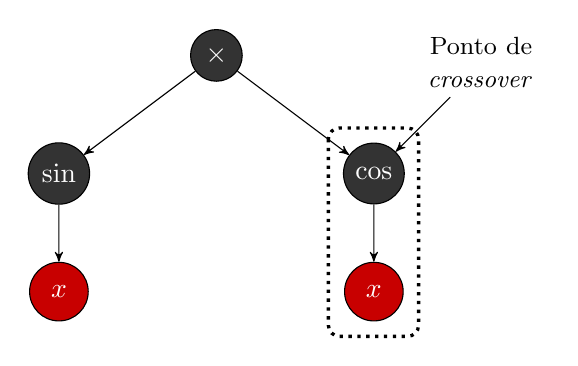
\begin{tikzpicture}[->,>=stealth',auto, remember picture,
        	black/.style={fill=my_black},
        	red/.style={fill=my_red, inner sep=5pt},
        	default/.style={draw, circle, text=white},
		    level 1/.style={sibling distance=40mm},
		    level 2/.style={sibling distance=20mm}]
		    \node [arn_r, default, black] {$\times$}
		    child{ node [arn_r, default, black] {$\sin$}
		        child{ node [arn_r, default, red] {$x$} }
		    }
		    child{ node [arn_r, default, black] (1AL) {$\cos$}
		        child{ node [arn_r, default, red] (2) {$x$} }
		    };
		    \node [draw=none, above right of=1AL, node distance=2cm, text width=4em] (xover-point) {\small
		    Ponto de \textit{crossover}};
		    \draw[draw] (xover-point) -- (1AL);
		    \draw[red, very thick, dotted, rounded corners, fill=none] ($(1AL.north west)+(-0.3,0.3)$) rectangle ($(2.south east)+(0.3,-0.3)$);
		\end{tikzpicture}
        \caption{Pai 1.}
        \label{fig:subtree-crossover-1}
    \end{subfigure}
    \hfill%
    \begin{subfigure}[b]{0.475\textwidth}
        \centering
    	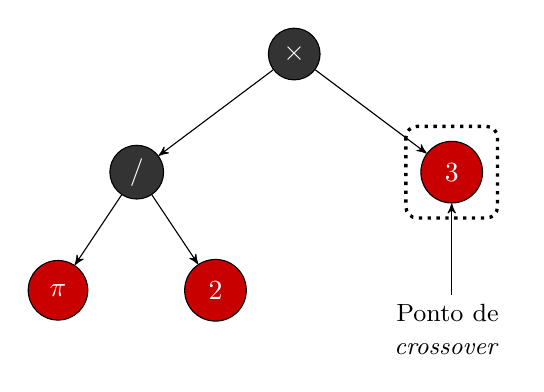
\begin{tikzpicture}[->,>=stealth',auto, remember picture,
	        black/.style={fill=my_black},
	        red/.style={fill=my_red, inner sep=5pt},
	        default/.style={draw, circle, text=white},
	        level 1/.style={sibling distance=40mm},
	        level 2/.style={sibling distance=20mm}]
	        \node [arn_r, default, black] {$\times$}
	        child{ node [arn_r, default, black] {$/$}
	            child{ node [arn_r, default, red] {$\pi$} }
	            child{ node [arn_r, default, red] {$2$} }
	        }
	        child{ node [arn_r, default, red] (1AR) {$3$} };
		    \node [draw=none, below of=1AR, node distance=2cm, text width=4em] (xover-point) {\small
		    Ponto de \textit{crossover}}; \draw[draw] (xover-point) -- (1AR);
		    \draw[red, very thick, dotted, rounded corners, fill=none] ($(1AR.north west)+(-0.3,0.3)$) rectangle ($(1AR.south east)+(0.3,-0.3)$) node (BB) {};
        \end{tikzpicture}
        \caption{Pai 2.}
        \label{fig:subtree-crossover-2}
    \end{subfigure}
	\vskip\baselineskip
	\begin{subfigure}[b]{0.475\textwidth}
        \centering
        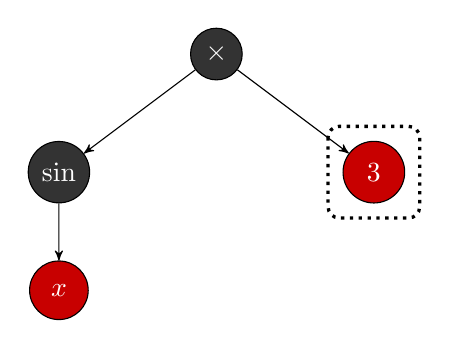
\begin{tikzpicture}[->,>=stealth',auto, remember picture,
        	black/.style={fill=my_black},
        	red/.style={fill=my_red, inner sep=5pt},
        	default/.style={draw, circle, text=white},
		    level 1/.style={sibling distance=40mm},
		    level 2/.style={sibling distance=20mm}]
		    \node [arn_r, default, black] {$\times$}
		    child{ node [arn_r, default, black] {$\sin$}
		        child{ node [arn_r, default, red] {$x$} }
		    }
		    child{ node [arn_r, default, red] (1BL) {$3$} };
		    \draw[red, very thick, dotted, rounded corners, fill=none] ($(1BL.north west)+(-0.3,0.3)$) rectangle ($(1BL.south east)+(0.3,-0.3)$);
		\end{tikzpicture}
        \caption{Filho 1.}
        \label{fig:subtree-crossover-3}
	\end{subfigure}
	\quad
	\begin{subfigure}[b]{0.475\textwidth}
        \centering
		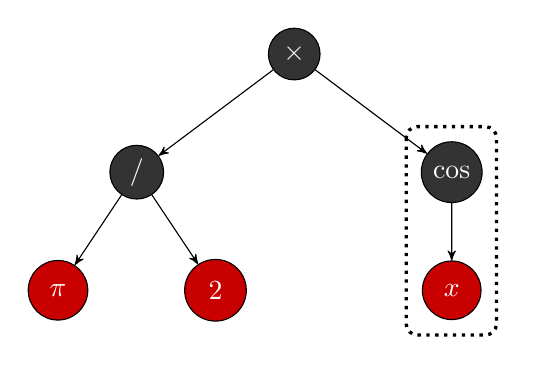
\begin{tikzpicture}[->,>=stealth',auto,
	        black/.style={fill=my_black},
	        red/.style={fill=my_red, inner sep=5pt},
	        default/.style={draw, circle, text=white},
	        level 1/.style={sibling distance=40mm},
	        level 2/.style={sibling distance=20mm}]
	        \node [arn_r, default, black] {$\times$}
	        child{ node [arn_r, default, black] {$/$}
	            child{ node [arn_r, default, red] {$\pi$} }
	            child{ node [arn_r, default, red] {$2$} }
	        }
            child{ node [arn_r, default, black] (1) {$\cos$}
                child{ node [arn_r, default, red] (2) {$x$} }
            };
		    \draw[red, very thick, dotted, rounded corners, fill=none] ($(1.north west)+(-0.3,0.3)$) rectangle ($(2.south east)+(0.3,-0.3)$) node (AA) {};
        \end{tikzpicture}
        \caption{Filho 2.}
        \label{fig:subtree-crossover-4}
	\end{subfigure}
    \begin{center}
        \makebox[\width]{Fonte: Autor.}
    \end{center}
\end{figure}

\subsection{Mutação}
O operador de mutação cria um filho ao realizar mudanças em um único pai \cite{poli2008,banzhaf1998,koza1992}. Seu modo de funcionamento gira em torno de um ponto de mutação. Este ponto, $p$, é escolhido aleatoriamente do pai selecionado, e a subárvore com raiz neste ponto é removida. Uma nova árvore gerada de forma aleatória é inserida no ponto $p$. Mutações podem causar um rápido crescimento e, portanto, um mecanismo de poda é empregado para garantir que a árvore não ultrapasse a profundidade máxima definida. A poda é realizada trocando as funções que estão na profundidade máxima por terminais. Diferentemente do operador de reprodução, a mutação é um operador global dado que subárvores aleatórias são criadas nos pontos de mutação, que podem resultar em diferenças significantes entre pais e filhos. Como consequência, este operador não promove convergência. A Figura \ref{fig:subtree-mutation} ilustra esse procedimento.

\begin{figure}[H]
    \caption{Exemplo de mutação de subárvores: \subref{fig:subtree-mutation-1} mostra o indivíduo escolhido para o processo de mutação, \subref{fig:subtree-mutation-2} apresenta uma nova subárvore gerada aleatoriamente e \subref{fig:subtree-mutation-3} mostra o indivíduo gerado pela mutação.}
    \label{fig:subtree-mutation}
    \begin{subfigure}[b]{0.33\textwidth}
        \centering
        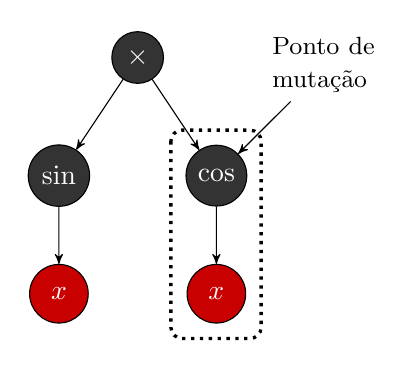
\begin{tikzpicture}[->,>=stealth',auto, remember picture,
        	black/.style={fill=my_black},
        	red/.style={fill=my_red, inner sep=5pt},
        	default/.style={draw, circle, text=white},
		    level 1/.style={sibling distance=20mm},
		    level 2/.style={sibling distance=20mm}]
		    \node [arn_r, default, black] {$\times$}
		    child{ node [arn_r, default, black] {$\sin$}
		        child{ node [arn_r, default, red] {$x$} }
		    }
		    child{ node [arn_r, default, black] (1AL) {$\cos$}
		        child{ node [arn_r, default, red] (2) {$x$} }
		    };
		    \node [draw=none, above right of=1AL, node distance=2cm, text width=4em] (xover-point) {\small
		    Ponto de mutação};
		    \draw[draw] (xover-point) -- (1AL);
		    \draw[red, very thick, dotted, rounded corners, fill=none] ($(1AL.north west)+(-0.3,0.3)$) rectangle ($(2.south east)+(0.3,-0.3)$);
		\end{tikzpicture}
		\caption{Pai.}
		\label{fig:subtree-mutation-1}
    \end{subfigure}
    %
    \begin{subfigure}[b]{0.30\textwidth}
        \centering
    	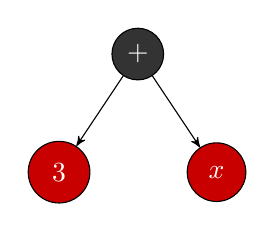
\begin{tikzpicture}[->,>=stealth',auto, remember picture,
        	black/.style={fill=my_black},
	        red/.style={fill=my_red, inner sep=5pt},
	        default/.style={draw, circle, text=white},
		    level 1/.style={sibling distance=20mm}]
	        \node [arn_r, default, black] {$+$}
		    child{ node [arn_r, default, red] {$3$} }
            child{ node (1) [arn_r, default, red] {$x$} };
	        \node [draw=none, below of=1, node distance=0.5cm] {};
        \end{tikzpicture}
		\caption{Subárvore aleatória.}
		\label{fig:subtree-mutation-2}
    \end{subfigure}
    %
    \begin{subfigure}[b]{0.33\textwidth}
	    \centering
        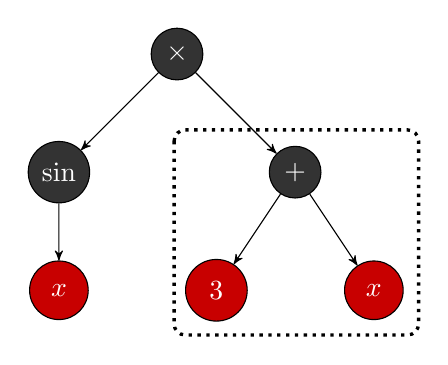
\begin{tikzpicture}[->,>=stealth',auto, remember picture,
        	black/.style={fill=my_black},
        	red/.style={fill=my_red, inner sep=5pt},
        	default/.style={draw, circle, text=white},
		    level 1/.style={sibling distance=30mm},
		    level 2/.style={sibling distance=20mm}]
		    \node [arn_r, default, black] {$\times$}
		    child{ node [arn_r, default, black] {$\sin$}
		        child{ node [arn_r, default, red] {$x$} }
		    }
		    %child{ node [arn_r, default, red] (1) {$3$} };
		    child{ node [arn_r, default, black] (1) {$+$}
		        child{ node [arn_r, default, red] {$3$} }
                child{ node [arn_r, default, red] (2) {$x$} }
            };
		    \draw[red, very thick, dotted, rounded corners, fill=none] ($(1.north west)+(-1.3,0.3)$) rectangle ($(2.south east)+(0.3,-0.3)$);
		\end{tikzpicture}
		\caption{Filho.}
		\label{fig:subtree-mutation-3}
	\end{subfigure}
    \begin{center}
        \makebox[\width]{Fonte: Autor.}
    \end{center}
\end{figure}

\section{Critérios de parada} \label{sec:termination}
\citeonline{koza1992} afirma que PG é ``um paradigma que é paralelo à natureza, tal que é um processo sem fim''. Claramente, é inviável manter um processo de computador executando sem um fim definido. Logo, o algoritmo de PG deve terminar assim que um predicado de sucesso é encontrado. Este predicado de sucesso pode ser definido de diferentes formas. Entretanto, a mais comum é encontrar a solução que contém taxas de acerto de 100\%, i.e., a solução perfeita para o problema. O predicado de sucesso pode ser dependente do problema e, assim, ser definido de forma diferente para cada problema \cite{poli2008}. Contudo, em alguns domínios de problemas a solução perfeita não é o desejado. Dessa forma, quando uma solução próxima do ótimo é encontrada, o algoritmo pode encerrar. Tipicamente, o melhor indivíduo da última geração do processo evolutivo é designado como o resultado da realização do algoritmo, embora possam ser retornados outros indivíduos para análise de suas estruturas e/ou valores de aptidão.

\section{\textit{Strongly-Typed Genetic Programming}} \label{sec:stgp}
\textit{Strongly-Typed Genetic Programming} (STGP) \cite{montana1995} é uma abordagem aprimorada de PG que impõe restrições sob os nós dentro de sua representação em árvore. Um tipo é alocado para cada terminal e função e, consequentemente, isto garante que as árvores sejam sintaticamente corretas durante o processo da evolução. STGP garante que durante a criação da população inicial e aplicação dos operadores genéticos, os tipos das funções e terminais são respeitados e não violados. Adicionalmente, ela reduz o tamanho do espaço de busca ao limitar as diferentes combinações de funções e terminais \cite{montana1995}.

Como exemplo, a função \textit{if-then-else} é uma que requer o uso de STGP. Esta função é ilustrada na Figura \ref{fig:stgp-example}, onde cada um dos três argumentos podem ter uma restrição de tipo. A função \textit{if-then-else} tem uma condição (\textit{if}) e duas consequências (\textit{then} e \textit{else}) que são realizadas baseadas no resultado da condição. Vamos assumir um tipo \textit{booleano} para o \textit{if}, como ilustrado na Figura \ref{fig:stgp-example}; como resultado da STGP, a condição \textit{if} sempre retornará um tipo \textit{booleano}, e esta imposição não pode ser violada. Logo, as variáveis $x$ e $y$ devem possuir tipo \textit{booleano}.

\begin{figure}[H]
    \caption{Função \textit{if-then-else}.}
    \label{fig:stgp-example}
    \begin{center}
        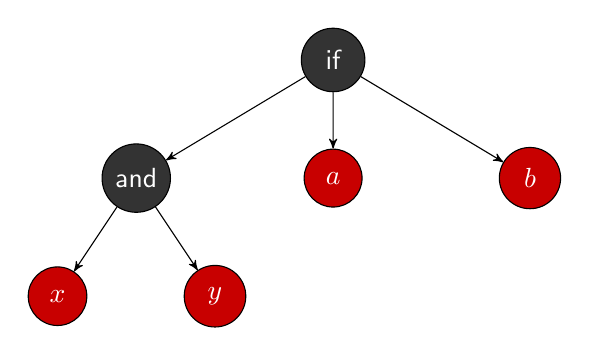
\begin{tikzpicture}[->,>=stealth',auto,
        	black/.style={fill=my_black},
        	red/.style={fill=my_red, inner sep=5pt},
        	default/.style={draw, circle, text=white, text centered},
		    level 1/.style={sibling distance=25mm},
		    level 2/.style={sibling distance=20mm}]
            \node [arn_r, default, black, inner sep=5pt] {if}
            child{ node [arn_r, default, black] {and}
                child{ node [arn_r, default, red] {$x$} }
                child{ node [arn_r, default, red] {$y$} }
            }
            child{ node [arn_r, default, red] {$a$} }
            child{ node [arn_r, default, red] {$b$} };
        \end{tikzpicture}
    \end{center}
    \begin{center}
        \makebox[\width]{Fonte: Autor.}
    \end{center}
\end{figure}

Ao aplicar os operadores genéticos, deve ser garantido que as atribuições de tipos não sejam violadas. Por exemplo: assumindo que na Figura \ref{fig:stgp-example}, o terminal $x$ é selecionado como ponto de mutação, deve ser garantido que a nova subárvore criada neste ponto retorne um valor \textit{booleano}. Se o valor de tipo atribuído é violado, a árvore é inválida.

\section{\textit{Bloat growth}} \label{sec:bloat-growth}
Antes de introduzir o conceito de \textit{bloat}, deve ser introduzido o conceito de íntrons. Íntrons são definidos como códigos redundantes em indivíduos de PG que não afetam seus valores de aptidão \cite{poli2008}. Em outras palavras, eles não afetam a sobrevivência dos indivíduos \cite{banzhaf1998}. Exemplos de íntrons são apresentados na Figura \ref{fig:introns}.

\begin{figure}[H]
    \centering
    \caption{Exemplos de íntrons: \subref{fig:introns-and} representa a expressão lógica $1 \wedge 1$ e \subref{fig:introns-or} representa a expressão lógica $0 \vee 0$.}
    \label{fig:introns}
    \begin{subfigure}[b]{0.5\linewidth}
        \centering
        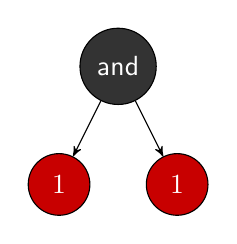
\begin{tikzpicture}[->,>=stealth',auto,
        	black/.style={fill=my_black},
        	red/.style={fill=my_red, inner sep=5pt},
        	default/.style={draw, circle, text=white, text centered},
		    level 1/.style={sibling distance=15mm}]
            \node [arn_r, default, black, inner sep=4pt] {and}
            child{ node [arn_r, default, red] {$1$} }
            child{ node [arn_r, default, red] {$1$} };
        \end{tikzpicture}
        \caption{}
        \label{fig:introns-and}
    \end{subfigure}%%
    \begin{subfigure}[b]{0.5\linewidth}
        \centering
        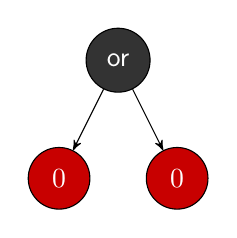
\begin{tikzpicture}[->,>=stealth',auto,
        	black/.style={fill=my_black},
        	red/.style={fill=my_red, inner sep=5pt},
        	default/.style={draw, circle, text=white, text centered},
		    level 1/.style={sibling distance=15mm}]
            \node [arn_r, default, black, inner sep=5pt] {or}
            child{ node [arn_r, default, red] {$0$} }
            child{ node [arn_r, default, red] {$0$} };
        \end{tikzpicture}
        \caption{}
        \label{fig:introns-or}
    \end{subfigure}
    \begin{center}
        \makebox[\width]{Fonte: Autor.}
    \end{center}
\end{figure}

\textit{Bloat} ocorre quando os indivíduos em uma população de PG crescem descontroladamente até alcançar as profundidades máximas das árvores. \citeonline{banzhaf1998} explica que o crescimento exponencial de íntrons leva ao \textit{bloat}. Caso não haja uma medida de prevenção, o \textit{bloat} com certeza ocorrerá. Dessa forma, pode-se afirmar que íntrons claramente têm efeito sobre o \textit{bloat}. Entretanto, pode ser argumentado que o crescimento exponencial dos íntrons age como uma espécie de proteção global \cite{banzhaf1998}. O operador de cruzamento pode ter um efeito destrutivo caso remova boas partes de um indivíduo. Este efeito pode ser reduzido se o operador de cruzamento remover um íntron de uma árvore ao invés de um bom bloco de construção. À medida que o algoritmo de PG itera, os indivíduos tornam-se mais aptos e, eventualmente, o algoritmo irá encontrar dificuldade em melhorá-los ainda mais. Uma vez que o \textit{bloat} ocorre, o algoritmo de PG irá tentar ao máximo melhorar a aptidão do atual melhor indivíduo encontrado. Logo, pode ser argumentado que íntrons têm um efeito positivo nos indivíduos. No entanto, eles consequentemente podem levar ao \textit{bloat}. \citeonline{luke2001} discutem diversos métodos de controle do \textit{bloat}.

\chapter{Métodos de \textit{Kernel} para Regressão} \label{chapter:kernel-methods}

Um dos principais desafios -- e objetivos -- do aprendizado de máquinas é encontrar informações inerentes de um problema, de forma que seu uso torne-se fator chave durante o processo de aprendizagem. Modelos lineares buscam tais informações através de correlações entre as características escolhidas para descrever o objeto de estudo. A teoria e gama de aplicações de modelos lineares têm sido bastante estudadas e analisadas por décadas, e hoje constituem um arcabouço bem definido no campo de AM. Entretanto, a grande ocorrência de fenômenos não-lineares em problemas do mundo real traz a necessidade de criação de modelos mais complexos.

Ao decorrer das últimas décadas, o uso de métodos de \textit{kernel} tem se mostrado bem sucedido ao permitir a criação de extensões não-lineares de clássicos modelos lineares \cite{abrahamsen2013}. A ideia básica por trás de métodos de \textit{kernel} é realizar um mapeamento do problema original para um espaço de alta -- ou até infinita -- dimensão, chamado de espaço de características, onde métodos lineares são utilizados para buscar as relações entre os padrões. Embora seu uso tenha se popularizado em anos recentes, o trabalho inicial na área costuma ser creditado a \citeonline{aizerman1964}, que utilizando o teorema de Mercer e RKHS, criaram algo muito próximo do que hoje é chamado de truque do \textit{kernel} \cite{schlkopf2004}.

O truque do \textit{kernel} permite a criação de eficientes métodos aplicáveis tanto para problemas de aprendizagem supervisionada quanto não-supervisionada. De particular interesse desta monografia, são as aplicações em problemas de regressão. Entre os métodos estado-da-arte, os membros mais conhecidos são: (\textit{i}) \textit{support vector regression} (SVR) \cite{smola1997}, cuja formulação é derivada da teoria do aprendizado estatístico \cite{vapnik1995,vapnik1998}; (\textit{ii}) \textit{least squares support vector regression} (LSSVR), cuja construção é uma simplificação daquela usada nas SVR; (\textit{iii}) \textit{kernel ridge regression} (KRR) \cite{saunders1998}, que possui uma formulação semelhante à das LSSVR; e por fim, (\textit{iv}) \textit{gaussian processes} (GP) \cite{rasmussen2006}, cuja formulação advém da teoria dos processos estocásticos.

Este capítulo descreve como a teoria de métodos de \textit{kernel} é utilizada no contexto da \textit{\textit{ridge regression}} para a criação do método KRR. Para isso, a seção \ref{sec:linreg} discute modelos de regressão linear, bem como apresenta como o método dos mínimos quadrados é utilizado para estimar %-- de maneira não-enviesada --
os coeficientes de regressão. A seção \ref{sec:ridge} apresenta a \textit{ridge regression} como um método de penalização da soma dos erros quadráticos. Na seção \ref{sec:kernel-trick} é mostrado como o truque do \textit{kernel} é utilizado para a formulação do KRR. Por fim, a seção \ref{sec:gkr} apresenta a proposta deste trabalho, denominada \textit{Genetic Kernels for Regression} (GKR).

\section{Regressão linear} \label{sec:linreg}
% Análise de regressão é uma técnica de estatística para investigação e modelagem de relacionamentos entre variáveis \cite{montgomery2012}. Através dessas variáveis podemos representar o comportamento de um objeto de interesse. Um dos modelos mais simples e utilizados para análise de regressão é descrito pela equação
Modelos de regressão são procedimentos estatísticos que permitem estimar relações entre variáveis, onde através destas podemos representar o comportamento de um objeto de interesse. Um dos modelos mais utilizados em problemas de regressão é descrito como

\begin{equation}
    \label{ch2:eq1}
    y = f(\mathbf{x}) = \mathbf{w}^{\top}\mathbf{x} = \sum_{i=1}^{p}{w_i \cdot x_i}
\end{equation}

Usualmente, variáveis à esquerda ($y$) da equação de regressão são chamadas de variáveis dependentes, enquanto as do lado direito ($\mathbf{x}$) são chamadas de variáveis independentes. Entretanto, \citeonline{montgomery2012} argumentam que tais nomenclaturas podem gerar confusão com o conceito de independência estatística. Dessa forma, nomearemos as variáveis da seguinte forma:

\begin{itemize}
    \item variáveis dependentes $\rightarrow$ variáveis de regressão;% (ou predição);
    \item variáveis independentes $\rightarrow$ variáveis de resposta.
\end{itemize}

De modo geral, o objetivo de um modelo de regressão é encontrar uma função que melhor interpole um conjunto de treinamento $\mathcal{D} = \{(\mathbf{x}_i, y_i)\}^{n}_{i=1}$ composto de pontos $\mathbf{x}_i$ extraídos de $\mathcal{X} \subseteq \mathbb{R}^p$ e $y_i$ extraídos de $\mathcal{Y} \subseteq \mathbb{R}$. Vale salientar que tanto neste capítulo, quanto no restante desta monografia, denotamos $\mathbf{x} = [x_1,x_2,\ldots,x_p]$ como o vetor de entrada p-dimensional e $\mathbf{w}^{\top}$ como o vetor transposto de $\mathbf{w} \in \mathbb{R}^p$. Quando a equação (\ref{ch2:eq1}) possui apenas uma variável de regressão, o modelo é chamado de \textbf{regressão linear simples}; quando possui duas ou mais variáveis, é chamado de \textbf{regressão linear múltipla}.

Em termos geométricos, um modelo de regressão linear posiciona um hiperplano de modo que este ajuste-se da melhor forma possível aos $n$ padrões de treinamento. A Figura \ref{fig:ch2-linreg} apresenta dois exemplos: \ref{fig:ch2-linreg1} caso unidimensional, $p = 1$, onde o hiperplano toma forma de uma linha reta; e \ref{fig:ch2-linreg2} caso bidimensional, $p = 2$, onde o hiperplano toma forma de um plano no $\mathbb{R}^2$.

\begin{figure}[ht]
    \caption{Hiperplanos obtidos por um modelo de regressão linear para funções que contém ruído, onde: \subref{fig:ch2-linreg1} apresenta a reta estimada para padrões unidimensionais descritos pela função $f(x) = 2x + 3$, e \subref{fig:ch2-linreg2} apresenta o plano estimado para padrões bidimensionais descritos pela função $f(x_1, x_2) = (3 - 2x_1 - 5x_2)/4$.}
    \label{fig:ch2-linreg}
    \begin{subfigure}[b]{0.49\linewidth}
        \centering
        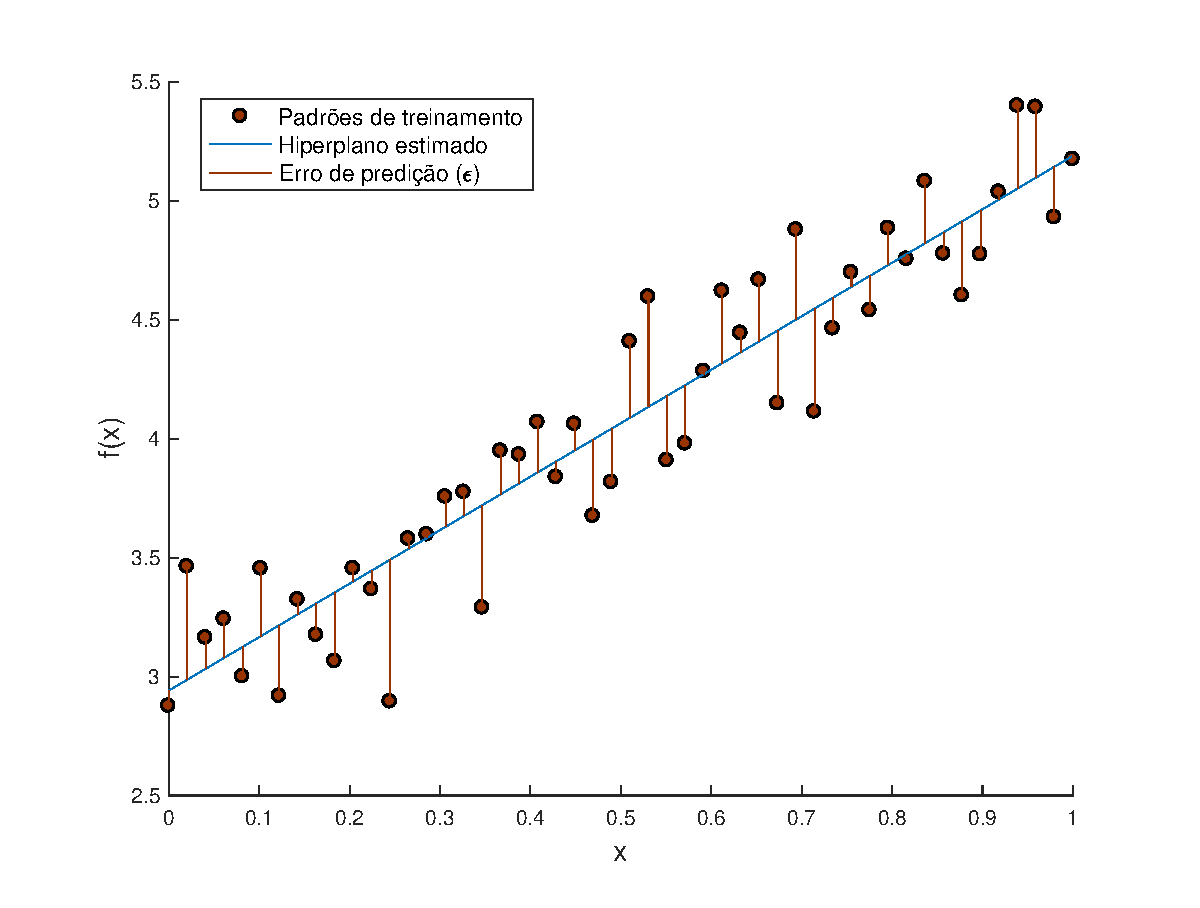
\includegraphics[width=\linewidth]{chapter2/tcc_2D.eps}
        \caption{}
        \label{fig:ch2-linreg1}
    \end{subfigure}%%
    \begin{subfigure}[b]{0.49\linewidth}
        \centering
        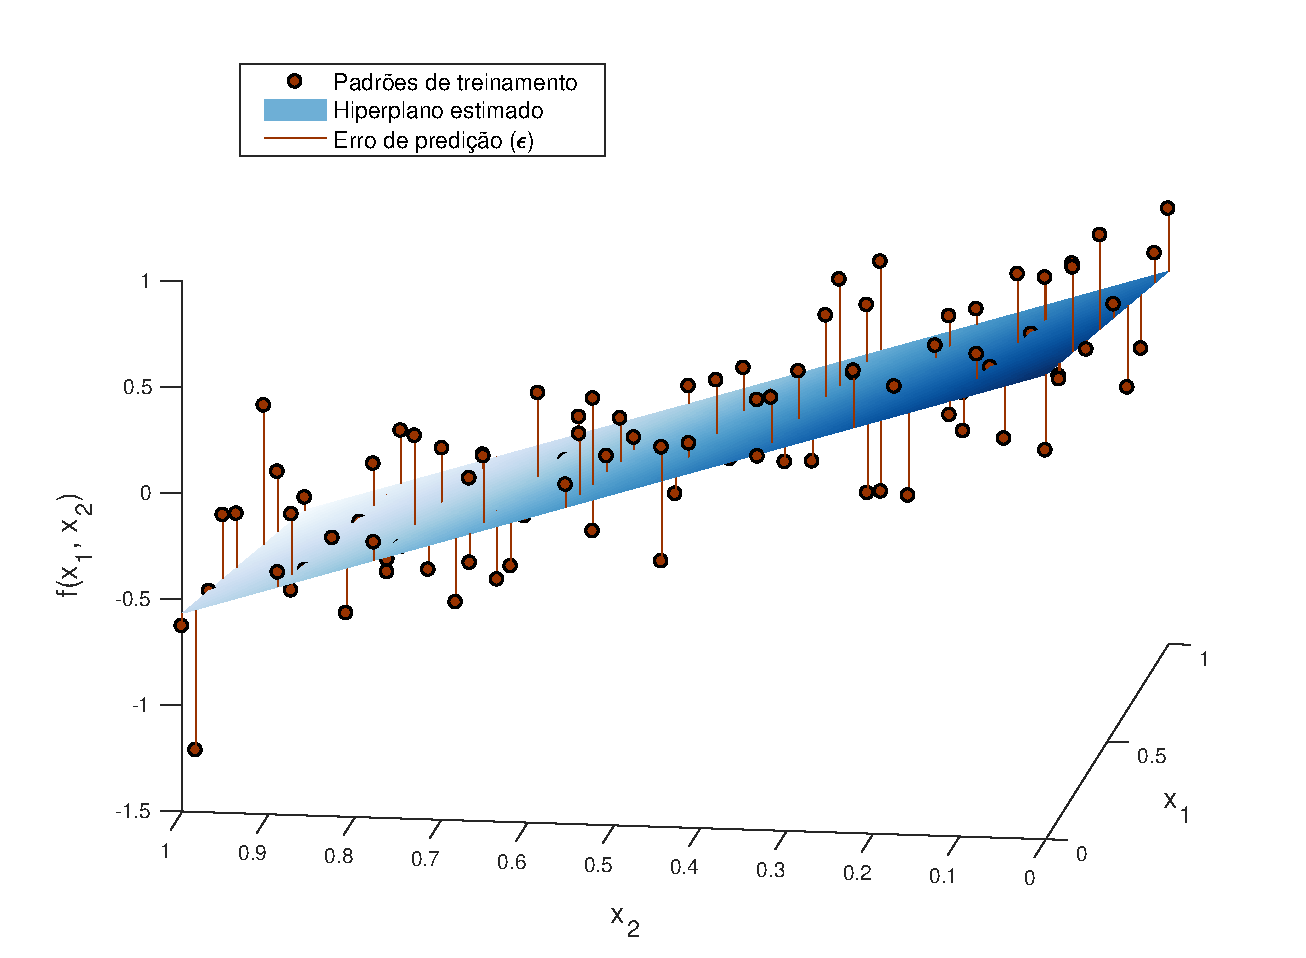
\includegraphics[width=\linewidth]{chapter2/tcc_3D.eps}
        \caption{}
        \label{fig:ch2-linreg2}
    \end{subfigure}
    \centering \makebox[\width]{Fonte: Autor.}
\end{figure}

Embora modelos de regressão sejam capazes de encontrar um hiperplano que represente -- da melhor forma possível -- o comportamento de um objeto de interesse, é comum que não o faça de forma exata. Uma justificativa para esta possibilidade é que modelos de regressão são modelos empíricos; ou seja, são capazes apenas de estimar o comportamento de modelos do mundo real \cite{montgomery2012}. Portanto, é necessário adicionar à equação (\ref{ch2:eq1}) uma medida de erro, que represente a diferença entre os valores observados de $y$ e os valores estimados pelo hiperplano $\mathbf{w}^{\top}\mathbf{x}$. Sumarizando, a equação (\ref{ch2:eq1}) é reescrita como

\begin{equation}
    \label{ch2:eq2}
    y = f(\mathbf{x}) = \mathbf{w}^{\top}\mathbf{x} + \epsilon = \sum_{i=1}^{p}{w_i \cdot x_i} + \epsilon.
\end{equation}

Para encontrar o hiperplano que melhor se ajustará aos padrões de treinamento, é necessário estimar os melhores valores para os parâmetros $w_i$, chamados de \textbf{coeficientes de regressão}. Quando os dados de treinamento são gerados na forma $(\mathbf{x}, f(\mathbf{x}))$, e há $n = p$ padrões linearmente independentes, é possível encontrar os coeficientes de regressão através da solução do sistema linear

\begin{equation}
    \label{ch2:eq3}
    \mathbf{X}\mathbf{w} = \mathbf{y},
\end{equation}

\noindent onde $\mathbf{X}$ é a matriz em que as linhas são formadas pelos padrões de treinamento $\mathbf{x}^{\top}_1,\ldots,\mathbf{x}^{\top}_n$, e $\mathbf{y}$ denota o vetor $[y_1,\ldots,y_n]^{\top}$ \cite{shawe2004}.

Entretanto, podem ocorrer casos em que o número de padrões não é igual a dimensão dos mesmos. Do mesmo modo, pode haver ruído durante o processo de coleta dos padrões, o que torna necessário o uso de outro método para encontrar os coeficientes de regressão. Dos diversos métodos propostos na literatura que são capazes de estimar os valores de cada coeficiente $w_i$, o mais utilizado é o dos mínimos quadrados (do inglês, \textit{least squares}), onde os valores escolhidos para cada coeficiente são aqueles que minimizam a soma de erros quadráticos, $\mathcal{L}(\mathcal{D}, \mathbf{w})$:

\begin{equation}
    \label{ch2:eq4}
    \mathcal{L}(\mathcal{D}, \mathbf{w}) = \sum_{i=1}^{n}{(y_i - f(\mathbf{x}_i))^2} = \sum_{i=1}^{n}{(y_i - \mathbf{w}^{\top}\mathbf{x}_i)^2} = \sum_{i=1}^{n}{\epsilon_{i}^2},
\end{equation}

\noindent onde $\epsilon_{i}^2$ denota o erro quadrático, ou perda quadrática, da estimativa de $f$ para o padrão $\mathbf{x}_i$. Logo, o aprendizado do modelo resume-se a encontrar o vetor $\mathbf{w}$ que minimiza a perda conjunta sobre os padrões de treinamento.

Utilizando notação matricial, podemos escrever o vetor de erros como

\begin{equation}
    \label{ch2:eq5}
    \boldsymbol{\epsilon} = \mathbf{y} - \mathbf{X}\mathbf{w},
\end{equation}

\noindent o que possibilita reescrever a equação (\ref{ch2:eq4}) como

\begin{align}
    \label{ch2:eq6}
    \mathcal{L}(\mathcal{D}, \mathbf{w})
    &= \boldsymbol{\epsilon}^{\top}\boldsymbol{\epsilon} \notag \\
    &= (\mathbf{y} - \mathbf{X}\mathbf{w})^{\top}(\mathbf{y} - \mathbf{X}\mathbf{w}) \notag \\
    &= \mathbf{y}^{\top}\mathbf{y} - \mathbf{w}^{\top}\mathbf{X}^{\top}\mathbf{y} - \mathbf{y}^{\top}\mathbf{X}\mathbf{w} + \mathbf{w}^{\top}\mathbf{X}^{\top}\mathbf{X}\mathbf{w} \notag \\
    &= \mathbf{y}^{\top}\mathbf{y} - 2\mathbf{w}^{\top}\mathbf{X}^{\top}\mathbf{y} + \mathbf{w}^{\top}\mathbf{X}^{\top}\mathbf{X}\mathbf{w}
\end{align}

Minimizar a soma de erros quadrados resume-se a derivar (\ref{ch2:eq6}) em relação a $\mathbf{w}$. Ou seja, o vetor $\mathbf{\hat{w}}$ estimado pelo método dos mínimos quadrados deve satisfazer

\begin{equation}
    \label{ch2:eq7}
    \frac{\partial \mathcal{L}}{\partial\mathbf{w}} = - 2\mathbf{X}^{\top}\mathbf{y} + 2\mathbf{X}^{\top}\mathbf{X}\mathbf{w} = \mathbf{0},
\end{equation}

\noindent que pode ser simplificado como

\begin{equation}
    \label{ch2:eq8}
    \mathbf{X}^{\top}\mathbf{X}\mathbf{w} = \mathbf{X}^{\top}\mathbf{y}.
\end{equation}

As equações (\ref{ch2:eq8}) são conhecidas como equações normais, umas vez que o vetor de erros $\boldsymbol{\epsilon}$ é ortogonal (ou normal) em relação ao hiperplano gerado \cite{bates1988}. Para solucionar as equações normais, podemos multiplicar ambos os lados de (\ref{ch2:eq8}) pela inversa de $\mathbf{X}^{\top}\mathbf{X}$, supondo que a matriz $(\mathbf{X}^{\top}\mathbf{X})^{-1}$ exista. Portanto, o vetor $\mathbf{\hat{w}}$ obtido é

\begin{equation}
    \label{ch2:eq9}
    \mathbf{\hat{w}} = (\mathbf{X}^{\top}\mathbf{X})^{-1}\mathbf{X}^{\top}\mathbf{y}.
\end{equation}

Por fim, a função de predição para novos padrões é dada por

\begin{equation}
    \label{ch2:eq10}
    f(\mathbf{x}) = \mathbf{\hat{w}}^{\top}\mathbf{x}.
\end{equation}

Modelos de regressão linear são bastante utilizados pela simplicidade em sua formulação, que permite fácil modelagem de relacionamentos das variáveis de interesse. Entretanto, existem problemas que possuem quantidades insuficientes de padrões para treinamento, ruído no processo de coleta dos dados, multicolinearidade, entre outros. Essas são algumas dificuldades tipicamente encontradas em problemas mal-condicionados. Uma abordagem frequentemente utilizada é restringir a escolha de funções para aquelas que possuem normas pequenas \cite{shawe2004}. Essa abordagem cria um critério de otimização conhecido como \textit{ridge regression}, discutido na seção \ref{sec:ridge}.

\section{\textit{Ridge regression}} \label{sec:ridge}
O método dos mínimos quadrados possui grande popularidade em áreas como estatística, otimização e aprendizado de máquina; em grande parte, isso deve-se a simplicidade de sua formulação matemática e à suas propriedades analíticas. Uma das propriedades mais interessantes é obtida através do teorema de Gauss-Markov, o qual diz que os coeficientes estimados pelos mínimos quadrados são os melhores estimadores lineares não-enviesados. Por ``melhores'', diz-se que possuem menor variância entre a classe de estimadores lineares não-enviesados, embora não haja garantia de que essa variância seja pequena \cite{montgomery2012}.

Diversos métodos foram propostos para solucionar este problema e, de modo geral, são chamados de métodos de redução (do inglês, \textit{shrinkage methods}). Um dos mais utilizados é a regressão \textit{ridge} (do inglês, \textit{ridge regression}) originalmente proposta por \apudonline[p. 305]{hoerl1970a}{montgomery2012} e que funciona como um método de penalização da soma de erros quadráticos, correspondendo a solucionar o problema de minimização

\begin{equation}
    \label{ch2:eq11}
    \min_{\mathbf{w}} \mathcal{L}_{\lambda}(\mathcal{D}, \mathbf{w}) = \min_{\mathbf{w}} \lambda \|\mathbf{w}\|^2 + \sum_{i=1}^{n}{(y_i - f(\mathbf{x}_i))^2},
\end{equation}

\noindent onde $\lambda$ é um número positivo que define o balanceamento entre a norma e o erro. Em outras palavras, $\lambda$ opera como um fator de regularização no método dos mínimos quadrados. Esta formulação da \textit{ridge regression} é chamada de formulação primal (ou método primal), pois define o espaço de soluções viáveis com base nas variáveis do problema original.

Seguindo \citeonline{shawe2004}, ao tomar a derivada de (\ref{ch2:eq11}) em relação a $\mathbf{w}$, obtemos as equações

\begin{equation}
    \label{ch2:eq12}
    \mathbf{X}^{\top}\mathbf{X}\mathbf{w} + \lambda\mathbf{w} = (\mathbf{X}^{\top}\mathbf{X} + \lambda\mathbf{I}_n)\mathbf{w} = \mathbf{X}^{\top}\mathbf{y},
\end{equation}

\noindent onde $\mathbf{I}_n$ é a matriz identidade $n \times n$. Neste caso, a matriz $(\mathbf{X}^{\top}\mathbf{X} + \lambda\mathbf{I}_n)$ é sempre invertível, dado que $\lambda > 0$. Dessa forma, o vetor de coeficientes $\mathbf{\hat{w}}$ é

\begin{equation}
    \label{ch2:eq13}
    \mathbf{\hat{w}} = (\mathbf{X}^{\top}\mathbf{X} + \lambda\mathbf{I}_n)^{-1}\mathbf{X}^{\top}\mathbf{y}.
\end{equation}

Solucionar a equação (\ref{ch2:eq13}) para $\mathbf{\hat{w}}$ envolve solucionar um sistema linear de $p \times p$ equações. A complexidade deste método é da ordem $\mathcal{O}(p^3)$, enquanto a função de predição para novos padrões é dada por

\begin{equation}
    \label{ch2:eq14}
    f(\mathbf{x}) = \mathbf{\hat{w}}^{\top}\mathbf{x}.
\end{equation}

\subsection{Formulação dual} \label{subsec:ridge-dual}
A formulação primal da \textit{ridge regression} nos permite inferir que o custo de encontrar os coeficientes $w_i$ depende diretamente da dimensionalidade, $p$, dos padrões. Em casos onde $p$ é muito grande, a solução da equação (\ref{ch2:eq13}) torna-se muito custosa computacionalmente. Entretanto, pode-se desenvolver uma formulação dual através dos multiplicadores de Lagrange, que expressa o vetor $\mathbf{w}$ como uma combinação linear dos padrões de treinamento.

Esta derivação segue os passos descritos por \citeonline{saunders1998}. Primeiramente, devemos reescrever a equação (\ref{ch2:eq11}) como

\begin{equation}
    \label{ch2:eq15}
    \begin{aligned}
        & \text{minimize}
        & & \lambda \|\mathbf{w}\|^2 + \sum_{i=1}^{n}{(y_i - f(\mathbf{x}_i))^2} \\
        & \text{sujeito a}
        & & \{y_i = \mathbf{w}^{\top}\mathbf{x}_i + \epsilon_i\}_{i=1}^{n}.
    \end{aligned}
\end{equation}

Utilizando as restrições descritas em (\ref{ch2:eq15}), podemos escrever o problema em sua forma dual através da construção do lagrangiano, que é dada por

\begin{equation}
    \label{ch2:eq16}
    L(\mathcal{D}, \mathbf{w}, \boldsymbol{\epsilon}, \boldsymbol{\alpha}) = \lambda \|\mathbf{w}\|^2 + \sum_{i=1}^{n}{\epsilon_i^{2} + \sum_{i=1}^{n} \alpha_i(y_i - \mathbf{w}^{\top}\mathbf{x}_i - \epsilon_i)},
\end{equation}

\noindent onde $\epsilon_i = y_i - f(\mathbf{x}_i)$ e $\boldsymbol{\alpha}$ é o vetor de coeficientes de Lagrange. O passo seguinte para obter a solução da equação (\ref{ch2:eq16}) é tomar os gradientes das variáveis primais iguais a zero, seguindo as condições de otimalidade de Karush-Kuhn-Tucker (KKT) \cite{boyd2004}.

Diferenciando $L(\mathcal{D}, \mathbf{w}, \boldsymbol{\epsilon}, \boldsymbol{\alpha})$ em relação a $\mathbf{w}$, obtemos

\begin{equation}
    \label{ch2:eq17}
    \mathbf{w} = \frac{1}{2\lambda} \sum_{i=1}^{n} \alpha_i \mathbf{x}_i.
\end{equation}

\noindent Substituindo (\ref{ch2:eq17}) em (\ref{ch2:eq16}), obtemos

\begin{align}
    \label{ch2:eq18}
    L(\mathcal{D}, \mathbf{w}, \boldsymbol{\epsilon}, \boldsymbol{\alpha}) 
    &= \frac{1}{4\lambda} \sum_{i=1}^{n} \sum_{j=1}^{n} \alpha_i \alpha_j (\mathbf{x}_i^{\top} \mathbf{x}_j) + \sum_{i=1}^{n} \epsilon_i^2 \notag \\
    &+ \frac{1}{2\lambda} \bigg{(}\sum_{i=1}^{n} \alpha_i \mathbf{x}_i\bigg{)}\bigg{(}-\sum_{i=1}^{n} \alpha_i \mathbf{x}_i\bigg{)} + \sum_{i=1}^{n} y_i \alpha_i - \sum_{i=1}^{n} \alpha_i \epsilon_i \notag \\
    &= -\frac{1}{4\lambda} \sum_{i=1}^{n} \sum_{j=1}^{n} \alpha_i \alpha_j (\mathbf{x}_i^{\top} \mathbf{x}_j) + \sum_{i=1}^{n} \epsilon_i^2 + \sum_{i=1}^{n} y_i \alpha_i - \sum_{i=1}^{n} \alpha_i \epsilon_i.
\end{align}

\noindent Diferenciando (\ref{ch2:eq18}) em relação a $\epsilon_i$, obtemos

\begin{equation}
    \label{ch2:eq19}
    \epsilon_i = \frac{\alpha_i}{2}, \quad i=1,\ldots,n.
\end{equation}

\noindent Através da equação (\ref{ch2:eq19}) pode-se inferir que a importância da i-ésima restrição é proporcional a seu respectivo erro. Ao substituir (\ref{ch2:eq19}) em (\ref{ch2:eq18}), temos que

\begin{equation}
    \label{ch2:eq20}
    \epsilon_i = -\frac{1}{4\lambda} \sum_{i=1}^{n} \sum_{j=1}^{n} \alpha_i \alpha_j (\mathbf{x}_i^{\top} \mathbf{x}_j) -\frac{1}{4} \sum_{i=1}^{n} \alpha_i^2 + \sum_{i=1}^{n} y_i \alpha_i.
\end{equation}

\noindent Denotando $K$ como a matriz $n \times n$ dos produtos internos \[ K_{ij} = \mathbf{x}_i^{\top}\mathbf{x}_j, \] e diferenciando (\ref{ch2:eq20}) em relação a $\alpha_i$, obtemos que

\begin{equation}
    \label{ch2:eq21}
    -\frac{1}{2\lambda} K\boldsymbol{\alpha} - -\frac{1}{2} \boldsymbol{\alpha} + \mathbf{y} = \mathbf{0},
\end{equation}

\noindent que é equivalente a 

\begin{equation}
    \label{ch2:eq22}
    \boldsymbol{\alpha} = 2\lambda(K + \lambda\mathbf{I}_n)^{-1}\mathbf{y}.
\end{equation}

\noindent Utilizando a equação (\ref{ch2:eq17}), podemos obter que a função de predição para novos padrões é

\begin{align}
    \label{ch2:eq23}
    f(\mathbf{x}) 
    &= \mathbf{w}^{\top}\mathbf{x} \notag \\
    &= \bigg{(} \frac{1}{2\lambda} \sum_{i=1}^{n} \alpha_i \mathbf{x}_i \bigg{)} \mathbf{x} \notag \\
    &= \frac{1}{2\lambda} \boldsymbol{\alpha} \mathbf{k} \notag \\
    &= \mathbf{y}^{\top}(K + \boldsymbol{\alpha}\mathbf{I}_n)^{-1}\mathbf{k},
\end{align}

\noindent onde $\mathbf{k} = [k_1,\ldots,k_n]^{\top}$ é o vetor dos produtos internos: \[ k_i = \mathbf{x}_i^{\top}\mathbf{x}, \quad i = 1,\ldots,n. \]

\section{O truque do \textit{kernel}} \label{sec:kernel-trick}
Até o presente momento, as formulações dos mínimos quadrados e da \textit{ridge regression} tinham como objetivo encontrar relações lineares entre as variáveis de um problema. As funções que permitem modelar problemas de regressão devem, então, ser lineares ou uma aproximação linear razoável \cite{hastie2009}. Contudo, a grande maioria dos problemas do mundo real possui natureza não-linear, de forma que estimativas mais precisas de $y$ só podem ser obtidas através do uso de uma função (ou combinação de funções) não-linear.

Uma estratégia interessante que tornou-se bastante popular, consiste em mapear os padrões para um espaço de Hilbert de alta (ou até infinita) dimensão, onde as relações tornam-se lineares e, consequentemente, seja possível aplicar modelos como a \textit{ridge regression}. Os mapeamentos considerados são da forma

\begin{equation}
    \label{ch2:eq24}
    \mathbf{\phi} : \mathbf{x} \mapsto \mathbf{\phi}(\mathbf{x}) \in \mathcal{H}.
\end{equation}

% \noindent O objetivo do mapeamento $\phi$ é converter o problema não-linear em um problema linear.
\noindent A consequência disso é vista sobre o conjunto de treinamento, que deve ser reformulado como $\mathcal{D} = \{(\phi(\mathbf{x}_i), y_i)\}^{n}_{i=1}$. Dessa forma, o modelo descrito na equação (\ref{ch2:eq2}) torna-se

\begin{equation}
    \label{ch2:eq25}
    y = f(\mathbf{x}) = \mathbf{w}^{\top} \phi(\mathbf{x}) + \epsilon = \sum_{i=1}^{p}{w_i \cdot \phi(x_i)} + \epsilon
\end{equation}

O uso da ``versão primal'' da \textit{ridge regression}, apesar de possível, pode tornar-se inviável em termos computacionais, por causa da ``maldição da dimensionalidade'' (do inglês, \textit{curse of dimensionality}). Em suma, o fato de haver funções não-lineares que operam em espaços de dimensão infinita torna inviável o uso da \textit{ridge regression} em sua forma primal, pois o modelo de computação atual não opera com o conceito de infinitude. Entretanto, a formulação dual traz a grande vantagem de não precisar representar os padrões de forma explícita no espaço $ \mathcal{H}$, chamado de espaço de características; são necessários apenas os produtos internos entre os pares de padrões

\begin{equation}
    \label{ch2:26}
    K_{ij} = \phi(\mathbf{x}_i)^{\top} \phi(\mathbf{x}_j).
\end{equation}

À esse atalho é dado o nome truque do \textit{kernel} (do inglês, \textit{kernel trick}). A Figura \ref{fig:kernel-trick} ilustra a ideia básica do truque do \textit{kernel}, onde os padrões $\mathbf{x} \in \mathcal{X}$ são mapeados para um espaço de Hilbert, $\mathcal{H}$, onde relações lineares são descobertas e consequentemente, equivalem a predições precisas no espaço original, $\mathcal{X}$. Uma função que realiza o mapeamento dos padrões para um espaço de Hilbert é chamada \textbf{função de \textit{kernel}}.

\begin{definition}[Função de \textit{Kernel}]
\label{def:kernel-function}
Um \textit{kernel} é uma função $\kappa$ que para todo $\mathbf{x}, \mathbf{z} \in \mathcal{X}$ satisfaz \[\kappa(\mathbf{x}, \mathbf{z}) = \phi(\mathbf{x})^{\top} \phi(\mathbf{z}), \] onde $\phi$ é uma função de mapeamento de $\mathcal{X}$ para um espaço característico $\mathcal{H}$ \[\mathbf{\phi} : \mathbf{x} \mapsto \mathbf{\phi}(\mathbf{x}) \in \mathcal{H}.\]
\end{definition}

\begin{figure}[H]
    \centering
    \caption{Ilustração da ideia básica em métodos de \textit{kernel}. Ao escolher um mapeamento adequado, os padrões são embutidos em um RKHS, $\mathcal{H}$, onde as relações são lineares. Predições no espaço $\mathcal{H}$ equivalem, então, a predições no espaço original, $\mathcal{X}$. A função de mapeamento, $\phi$, pode ser definida implicitamente através da escolha do \textit{kernel}.}
    \label{fig:kernel-trick}
    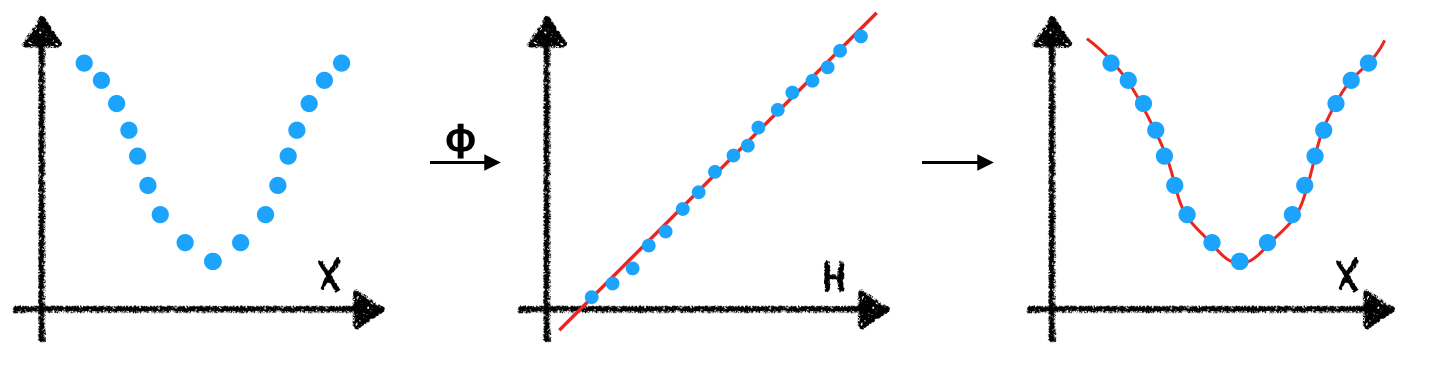
\includegraphics[width=\linewidth]{figures/images/kernel-example.png}
    \makebox[\width]{Fonte: Autor.}
\end{figure}

Utilizando-se do truque do \textit{kernel}, podemos redefinir a equação (\ref{ch2:eq16}), referente ao lagrangiano da \textit{ridge regression}, para

\begin{equation}
    \label{ch2:27}
    L(\mathcal{D}, \mathbf{w}, \boldsymbol{\epsilon}, \boldsymbol{\alpha}) = \lambda \|\mathbf{w}\|^2 + \sum_{i=1}^{n}{\epsilon_i^{2} + \sum_{i=1}^{n} \alpha_i(y_i - \mathbf{w}^{\top}\phi(\mathbf{x}_i) - \epsilon_i)}
\end{equation}

Finalmente, a nova função de predição é descrita como

\begin{equation}
    \label{ch2:eq29}
    f(\mathbf{x}) = \mathbf{y}^{\top}(K + \boldsymbol{\alpha}\mathbf{I}_n)^{-1}\mathbf{k},
\end{equation}

\noindent onde $\mathbf{K}$ é a matriz de produtos internos dos vetores $\phi(\mathbf{x}_i), \ldots, \phi(\mathbf{x}_n)$, resultados da aplicação da função de \textit{kernel} $\kappa$ sobre os padrões de treinamento, e $\mathbf{k}$ é o vetor de produtos internos: \[ k_i = \phi(\mathbf{x}_i)^{\top}\mathbf{x}, \quad\quad i = 1,\ldots,n. \]

Da equação (\ref{ch2:eq29}) surge o modelo conhecido como \textit{kernel ridge regression} (KRR), que será utilizado no decorrer desta monografia.

Vários métodos de \textit{kernel} tornam-se um problema de otimização no espaço de Hilbert, $\mathcal{H}$. Do teorema do representante (\textit{representer theorem}) \cite{aronszajn1950,scholkopf2001} segue que, embora o problema seja definido em um RKHS de alta (ou infinita) dimensão, sua solução permanece no subespaço $p$-dimensional definido pela extensão dos \textit{kernels} centrados nos $n$ padrões de treinamento. Considerando os cômputos de $\phi$ da ordem $\mathcal{O}(n)$, pode-se afirmar que o custo assintótico do cômputo dos coeficientes de Lagrange é da ordem $\mathcal{O}(n^3 + n^2p)$, enquanto o custo de predição é da ordem $\mathcal{O}(np)$. Apesar de possuir um custo assintótico maior, a formulação dual permite computar os produtos internos de modo mais eficiente que a formulação primal, já que não é necessário computar o mapeamento $\phi$ de maneira explícita. Dessa forma, a dual apresenta-se como uma representação mais eficiente que a primal.

% Para uma visão mais aprofundada (e teórica) sobre métodos de \textit{kernel}, recomenda-se a leitura dos textos \cite{smola1998learning,shawe2004,hofmann2008kernel,scholkopf2001}.

% O próprio termo \textit{kernel} pode conter diversos significados, quando aplicado em diferentes contextos.

% \section{Algumas propriedades de \textit{kernels}} \label{sec:kernel-properties}

\section{\textit{Genetic Kernels for Regression} (Proposta)} \label{sec:gkr}
Encontrar uma função de \textit{kernel} que se adapte a um determinado problema é um estágio crítico no desenvolvimento de métodos de aprendizagem baseados em \textit{kernel}. Isso se deve muito ao fato da necessidade de haver conhecimento \textit{a priori} sobre o problema \cite{shawe2004}. De acordo com \citeonline{scholkopf2001}, a própria escolha do \textit{kernel} representa conhecimento sobre o problema e sua solução. Como já mencionado no Capítulo \ref{chapter:introduction}, uma abordagem bastante utilizada na comunidade acadêmica é utilizar \textit{kernels} já consolidados na literatura, apenas realizando uma busca pelo seu melhor conjunto de parâmetros. A Tabela \ref{tab:commom-kernels} apresenta uma lista das principais funções de \textit{kernels} utilizados e seus respectivos parâmetros.

\begin{table}[H]
    \caption{Funções de \textit{kernel} mais populares na literatura.}
    \begin{center} \label{tab:commom-kernels}
        \begin{tabular}{l@{\hskip 20pt}l}
            \hline\noalign{\smallskip}
            \textbf{\textit{Kernel}} & \textbf{Descrição} \\
            \noalign{\smallskip}
            \hline
            \noalign{\smallskip}
            Linear		& $\kappa({\mathbf x}$,${\mathbf z}$) $= \mathbf{x}^{\top}\mathbf{z}$ \\
            RBF	        & $\kappa({\mathbf x}$,${\mathbf z}$) $= e^{-\|\mathbf{x} - \mathbf{z}\|^2 / \sigma^2}$, onde $\sigma$ é uma constante. \\
            Polinomial	& $\kappa({\mathbf x}$,${\mathbf z}$) $= (\mathbf{x}^{\top}\mathbf{z} + 1)^d$, onde $d$ é o grau do polinômio. \\
            \hline
        \end{tabular}
    \end{center}
    \begin{center}
        \makebox[\width]{Fonte: \citeonline{ajalmar2011}}.
    \end{center}
\end{table}

% Como alternativa, duas outras abordagens são encontradas na literatura. A primeira concentra-se no aprendizado de \textit{kernels} a partir do conjunto de dados. Essa abordagem funciona através da definição de um conjunto de \textit{kernels}
% (\textit{Multiple Kernel Learning}, MKL)

Criar \textit{kernels} que adaptem-se a problemas específicos é uma opção mais conveniente, pois o projetista de um modelo baseado em \textit{kernels} não necessita verificar qual \textit{kernel} é melhor para o problema que deve ser solucionado. Entretanto, projetar uma função de \textit{kernel} demanda muito conhecimento acerca do problema, de forma que torna-se muito custoso (em termos de tempo dispendido) realizar esta tarefa manualmente. Uma alternativa é a utilização da construção em blocos. Esse modelo de construção utiliza propriedades de fechamento sobre as funções de \textit{kernel} que permite que novas funções sejam geradas a partir da combinação de outras já conhecidas. A Proposição \ref{prop:1}, adaptada de \cite{shawe2004} lista três operações de fechamento que garantem a construção de novas funções de \textit{kernel} válidas.
% Uma alternativa, que vem ganhando bastante popularidade em anos recentes, é a criação de funções de \textit{kernel} específicas para determinados tipos de problemas. Uma forma possível de criação de novos \textit{kernels} é a utilização da construção em blocos. Esse modelo de construção utiliza propriedades de fechamento sobre as funções de \textit{kernel} que permite que novas funções sejam geradas a partir da combinação de outras já conhecidas. A Proposição \ref{prop:1}, adaptada de \cite{shawe2004} lista três operações de fechamento que garantem a construção de novas funções de \textit{kernel} válidas.

\begin{proposition}[Propriedades de fechamento]
    \label{prop:1}
    Sejam $\kappa_1$ e $\kappa_2$ dois kernels sobre $\mathbf{X} \times \mathbf{X}, \mathbf{X} \subseteq
    \mathbb{R}^n$ e $a \in \mathbb{R}^+$. Então as seguintes funções são kernels

    \begin{enumerate}[label=(\roman*)]
        \item $\kappa(\mathbf{x},\mathbf{z}) = \kappa_1(\mathbf{x},\mathbf{z}) + \kappa_2(\mathbf{x},\mathbf{z})$,
        \item $\kappa(\mathbf{x},\mathbf{z}) = \kappa_1(\mathbf{x},\mathbf{z}) \times \kappa_2(\mathbf{x},\mathbf{z})$,
        \item $\kappa(\mathbf{x},\mathbf{z}) = a \cdot \kappa_2(\mathbf{x},\mathbf{z})$.
        % \item $k(\mathbf{x},\mathbf{z}) = e^{\kappa_1(\mathbf{x},\mathbf{z})}$.
    \end{enumerate}
\end{proposition}

A proposta deste trabalho, denominada \textit{Genetic Kernels for Regression} (GKR), baseia-se em PG para encontrar \textit{kernel}(\textit{s}) para quaisquer problemas de regressão a serem solucionados pelo método KRR. Como entrada, o GKR recebe o parâmetro de regularização $\lambda$, e um conjunto de dados de treinamento $\mathcal{D}$. Ao fim de sua realização, o algoritmo retorna o melhor \textit{kernel} encontrado, que será usado na construção do modelo de predição final.

Inicialmente, uma população de soluções é construída de forma aleatória, tal que cada indivíduo representa um \textit{kernel} construído utilizando as propriedades apresentadas na Proposição \ref{prop:1} e os \textit{kernels} apresentados na Tabela \ref{tab:gkr-kernels}. A avaliação dos indivíduos se dá através da raiz da média dos erros quadráticos (\textit{Root Mean Squared Error}, RMSE). As gerações seguintes são criadas a partir da aplicação dos operadores genéticos (seção \ref{sec:genetic-operators}) sobre os melhores indivíduos da atual população, escolhidos com base em seus valores de aptidão. Este processo é repetido até que um dos critérios de parada seja atendido. Ao fim do processo evolutivo, o melhor indivíduo da população final é escolhido para a criação do modelo final. A Figura \ref{fig:gkr-overview} apresenta uma visualização do fluxo de trabalho do GKR.

\begin{figure}[H]
    \caption{Fluxo de trabalho do algoritmo GKR.}
    \centering
    \label{fig:gkr-overview}
    \begin{tikzpicture}[node distance = 4cm, auto,
        decision/.style={diamond, draw, fill=my_gray, text width=3em, text=white, aspect=1, text centered, node distance=3cm, inner sep=0pt},
        block inside/.style={rectangle, draw, fill=none, text width=8em, text centered, rounded corners, minimum height=3em}]

        \node [block] (dataset) {\scriptsize conjunto de dados de treinamento};
        \node [block, right of=dataset] (lambda) {\scriptsize parâmetro de regularização};
        \node [block inside, node distance=2.5cm, below of=dataset] (init) {\scriptsize criar população inicial de soluções};
        \node [block inside, node distance=2.5cm, below of=init] (fitness) {\scriptsize avaliar população de indivíduos};
        \node [decision, below of=fitness, node distance=2.5cm] (decide) {\scriptsize \textbf{D}};
        \node [block inside, right of=decide, node distance=5cm] (selection) {\scriptsize selecionar indivíduos};
        \node [block inside, above of=selection, node distance=2.5cm] (update) {\scriptsize atualizar população};
        \node [block inside, right of=update, node distance=4.5cm] (breeding) {\scriptsize aplicar operadores genéticos};
        \node [block inside, below of=decide, node distance=2.5cm] (bestsofar) {\scriptsize melhor indivíduo};
        \node [block, below of=bestsofar, node distance=2.5cm] (kernel) {\scriptsize função de \textit{kernel}};
        \node [decision, right of=bestsofar, text width=2em, node distance=9.2cm] (decide2) {\tiny \textbf{D}};
        \node [draw=none, right of=decide2, node distance=1.3cm, text width=4em, text centered] (end) {\tiny terminar busca?};

        \draw[very thick, dashed, rounded corners] ($(init.north west)+(-0.4,0.4)$) rectangle ($(end.south east)+(0.2,-0.7)$) node[text=black] at ($(breeding.north east)+(-0.2,3.2)$, 0) {\scriptsize \textbf{GKR}};
        \path [line] (dataset) -- (init);
        \path [line] (lambda) |- (init);
        \path [line] (init) -- (fitness);
        \path [line] (fitness) -- (decide);
        \path [line] (selection.east) -| (breeding.south);
        \path [line] (decide) -- node {\tiny não} (selection);
        \path [line] (decide) -- node {\tiny sim} (bestsofar);
        \path [line] (breeding) -- (update);
        \path [line] (update) -- (fitness);
        \path [line] (bestsofar) -- (kernel);
    \end{tikzpicture}
    \makebox[\width]{Fonte: Autor.}
\end{figure}

% Um potencial problema que pode surgir durante a execução do algortimo da PG, é o que muito autores chamam de \textit{bloat}. Esse fenômeno faz com as árvores geradas cresçam sem que se tenha aumento na peformance. Por essa razão, pretende-se utilizar o método de seleção \textit{lexictour}, que tem preferência por indivíduos de menor tamanho caso haja empate de performance entre vários indivíduos.

% Para determinar o quão apto é um indivíduo, uma validação cruzada será utilizada sobre seu RMSE (\textit{root mean squared error}). Antes do processo de evolução de uma geração iniciar, algumas configurações importantes são feitas. O conjunto de dados é dividido em dois subconjuntos: treinamento e teste. O conjunto de treinamento, então, é dividido em 10 partes (\textit{folds}). O treinamento de cada indivíduo é executado durante 10 iterações, sempre deixando um \textit{fold} como um conjunto de validação independente. A aptidão de um indivíduo é dada pela média das 10 validações.

% Nosso método terá sua performance comparada com uma SVM treinada com kernels clássicos (linear, gaussiano e polinomial) e as redes neurais MLP e RBF. Vale salientar que o processo de validação cruzada é o mesmo para todas as técnicas, ou seja, todas são treinadas, validadas e testadas com a mesma divisão do conjunto de dados. Essa escolha permite que as comparações de performance sejam mais precisas.

\subsection{Representação genética e população inicial}
Como já discutido no Capítulo \ref{chapter:genetic-programming}, a representação genética de um indivíduo é uma das partes cruciais no projeto de um algoritmo de PG. Anteriormente à decisão de qual estrutura será escolhida para representação de um indivíduo, é necessário que se decida qual será o conjunto primitivo a ser utilizado; ou seja, é necessário a definição dos conjuntos de funções e terminais. O conjunto de terminais é composto pelo conjunto de dados específico de cada problema, representado pela matriz $\mathbf{X}$, das variáveis de cada \textit{kernel} (tais como $\sigma$, a abertura da gaussiana), e de constantes efêmeras. O conjunto de funções escolhido é uma união entre os operadores apresentados na Proposição \ref{prop:1} e os \textit{kernels} listados na Tabela \ref{tab:gkr-kernels}.

\begin{table}[H]
    \caption{Funções de \textit{kernel} utilizados pelo GKR.}
    \begin{center} \label{tab:gkr-kernels}
        {
        \def\arraystretch{1.8}\tabcolsep=10pt
        \begin{tabular}{l@{\hskip 18pt}l}
            \hline\noalign{\smallskip}
            \textbf{\textit{Kernel}} & \textbf{Equação} \\
            \noalign{\smallskip}
            \hline
            \noalign{\smallskip}
            Cauchy 		            & $\kappa(\mathbf{x},\mathbf{z}) = \frac{1}{1 + \frac{\|\mathbf{x} - \mathbf{z}\|^2}{\sigma^2}}$ \\
            Exponential             & $\kappa(\mathbf{x},\mathbf{z}) = e^{-\frac{\|\mathbf{x} - \mathbf{z}\|}{\sigma^2}}$ \\
            Inverse Multiquadratic  & $\kappa(\mathbf{x},\mathbf{z}) = \frac{1}{\sqrt{\|\mathbf{x} - \mathbf{z}\|^2 + c^2}}$ \\
            Laplace		            & $\kappa(\mathbf{x},\mathbf{z}) = e^{-\frac{\|\mathbf{x} - \mathbf{z}\|}{\sigma}}$ \\
            Linear		            & $\kappa(\mathbf{x},\mathbf{z}) = \mathbf{x}^{\top}\mathbf{z}$ \\
            Multiquadratic          & $\kappa(\mathbf{x},\mathbf{z}) = \sqrt{\|\mathbf{x} - \mathbf{z}\|^2 + c^2}$ \\
            Polynomial	            & $\kappa(\mathbf{x},\mathbf{z}) = (\mathbf{x}^{\top}\mathbf{z} + 1)^d$ \\
            Rational Multiquadratic & $\kappa(\mathbf{x},\mathbf{z}) = 1 - \frac{\|\mathbf{x} - \mathbf{z}\|^2}{\|\mathbf{x} - \mathbf{z}\|^2 + c^2}$ \\
            RBF	                    & $\kappa(\mathbf{x},\mathbf{z}) = e^{-\frac{\|\mathbf{x} - \mathbf{z}\|^2}{\sigma^2}}$ \\
            Sigmoid         		& $\kappa(\mathbf{x},\mathbf{z}) = \tanh(a\mathbf{x}^{\top}\mathbf{z} + 1)$ \\
            \hline
        \end{tabular}
    }
    \end{center}
    \begin{center}
        \makebox[\width]{Fonte: Autor.}
    \end{center}
\end{table}

Vale salientar que, uma vez que as funções de \textit{kernel} recebem dois vetores como entrada (além de seu conjunto de parâmetros), é natural que se utilize uma matriz extra, $\mathbf{Z}$, que represente os padrões $\mathbf{z}$. Entretanto, como essas funções computam valores de similaridade entre padrões de um mesmo conjunto, tem-se que $\mathbf{Z} = \mathbf{X}$. A escolha pela utilização de duas matrizes, ao invés de apenas uma, é puramente por harmonia com a definição de função de \textit{kernel}. Entretanto, é possível a utilização apenas da matriz $\mathbf{X}$.

A representação genética de um indivíduo é a padrão da PG: árvores sintáticas. Para fins de exemplificação, a Figura \ref{fig:kernel-tree} mostra uma árvore que representa o kernel $Polynomial(\mathbf{X}, \mathbf{Z}, 7) + Linear(\mathbf{X}, \mathbf{Z})$.

Para criação da população inicial, foi utilizada a abordagem STGP. A justificativa para essa escolha encontra-se no fato de que, dado a natureza estocástica da PG, árvores sintaticamente inválidas podem ser criadas. Portanto, a STGP fornece um arcabouço robusto para definição de restrições dos tipos que um nó pode ter. Observe a Figura \ref{fig:kernel-tree} como exemplo: enquanto o nó que contém o \textit{kernel} linear só pode receber como entrada duas matrizes que representam o conjunto de dados, o kernel \textit{polinomial} pode receber uma entrada extra (o grau do polinômio, que possui valor inteiro). A Tabela \ref{tab:stgp-constraints} lista as restrições utilizadas para que o GKR crie árvores sintaticamente válidas.

% Tanto o processo de criação de uma árvore quanto o de alteração através dos operadores genéticos, deve obedecer a essas restrições, mantendo a árvore consistente.

% A população inicial é criada utilizando uma combinação das propriedades de fechamendo e das restrições de STGP para criar novas funções kernel válidas e que permaneçam consistentes ao longo do processo de evolução. A consistência de cada indivíduo é mantida porque em STGP, além das restrições padrões da PG, novas restrições são adicionadas a cada nó.

\begin{figure}[H]
    \caption{Exemplo de \textit{kernel} que pode ser criado pelo GKR. A árvore sintática representa a função $Pol(\mathbf{X}, \mathbf{Z}, 7) + Lin(\mathbf{X}, \mathbf{Z})$, onde $Pol=Polynomial$ e $Lin=Linear$.}
    \label{fig:kernel-tree}
    \begin{center}
        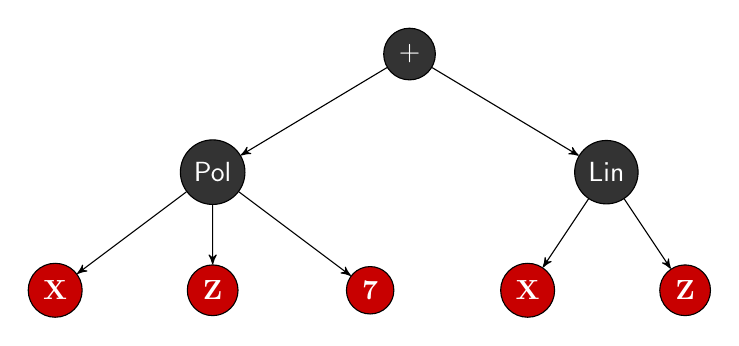
\begin{tikzpicture}[->,>=stealth',auto,
            black/.style={fill=my_black},
            red/.style={fill=my_red},
            default/.style={draw, circle, text=white},
            level 1/.style={sibling distance=50mm},
            level 2/.style={sibling distance=20mm}]
            \node [arn_r, default, black] {+}
            child{ node [arn_r, default, black] {Pol} 
                child{ node [arn_r, default, red] {$\mathbf{X}$} }
                child{ node [arn_r, default, red] {$\mathbf{Z}$} }
                child{ node [arn_r, default, red] {$\mathbf{7}$} }
            }
            child{ node [arn_r, default, black] {Lin}
                child{ node [arn_r, default, red] {$\mathbf{X}$} }
                child{ node [arn_r, default, red] {$\mathbf{Z}$} }
            };
        \end{tikzpicture}
    \end{center}
    \begin{center}
        \makebox[\width]{Fonte: Autor.}
    \end{center}
\end{figure}

\begin{table}[H]
    \caption{Restrições utilizadas pelo GKR para garantir que as árvores criadas sejam sintaticamente válidas.}
    \begin{center} \label{tab:stgp-constraints}
        \begin{tabular}{C@{\hskip 15pt}l}
            \hline\noalign{\smallskip}
            \textbf{Nó} & \textbf{Tipo} \\
            \noalign{\smallskip}
            \hline
            \noalign{\smallskip}
            $\sigma$ & Ponto flutuante \\
            $\mathbf{X}$ e $\mathbf{Z}$ & Matriz de pontos flutuantes \\
            $a$, $c$ e $d$ & Número inteiro \\
            \textit{Kernels} da Tabela \ref{tab:gkr-kernels} & \textit{kernel-function} \\
            Operadores da Proposição \ref{prop:1} & \textit{kernel-operator} \\
            \hline
        \end{tabular}
    \end{center}
    \begin{center}
        \makebox[\width]{Fonte: Autor.}
    \end{center}
\end{table}

\subsection{Função de aptidão e método de seleção}
Para o cálculo da aptidão de um indivíduo, é necessário que sejam computadas predições sobre um conjunto de dados não utilizado durante o treinamento. Isso é realizado através da separação do conjunto de dados de treinamento em dois subconjuntos: treinamento e validação. Detalhes sobre a metodologia de separação podem ser encontrados no Capítulo \ref{chapter:simulations}. A função de aptidão escolhida é a \textit{root mean square error} (RMSE):

\begin{equation}
    \label{ch3:eq29}
    RMSE = \sqrt{\frac{1}{n}\sum_{i=1}^{n}{(y_i - f(\mathbf{x}_i))^2}}
\end{equation}

Naturalmente, poderia ser utilizada a aptidão padronizada (veja seção \ref{sec:fitness-functions}). Entretanto, foi escolhido a aptidão ajustada por dois motivos: (\textit{i}) permite uma melhor separação entre as boas soluções das ótimas soluções, levando a um direcionamento mais preciso na busca pelo melhor indivíduo; e (\textit{ii}) permite usar o algoritmo padrão de PG, onde os melhores indivíduos são aqueles que possuem maiores valores de aptidão.

O método de seleção utilizado foi a seleção por torneio lexicográfico, proposto por \citeonline{luke2002}. Este operador modifica a seleção por torneio tradicional ao preferir árvores de menor profundidade quando dois ou mais indivíduos possuem o mesmo valor de aptidão (ou mesmo \textit{rank}). Este é um operador de seleção que vem sendo bastante utilizado no combate ao crescimento desenfreado do tamanho de um indivíduo, conhecido como \textit{bloat growth} (veja seção \ref{sec:bloat-growth}).

\subsection{Operadores genéticos}
Os operadores genéticos escolhidos são os mesmos descritos na seção \ref{sec:genetic-operators}.

\subsection{Critério de parada}
O algoritmo sempre é encerrado quando ocorre, pelo menos, uma das duas situações a seguir: (\textit{i}) um número predeterminado de gerações é atingido ou (\textit{ii}) a função de aptidão atinge seu valor máximo (ou seja, foi encontrado o \textit{kernel} ideal).

\chapter{Simulações Computacionais}\label{chapter:simulations}

Este capítulo apresenta a metodologia utilizada nas etapas de treinamento e teste do modelo GKR. Para isso, inicialmente são apresentados os conjuntos de dados utilizados para validação do desempenho. Para fins de comparação, são apresentados a metodologia e resultados dos seguintes métodos estado-da-arte: SVR, MLP e RBF.

A implementação do modelo GKR foi realizada utilizando a linguagem de programação Java\textsuperscript{TM} e a biblioteca de computação evolucionária ECJ (versão 23) \cite{luke2015}. Entretanto para o cômputo das aptidões dos indivíduos, bem como as implementações dos modelos SVR, MLP e RBF -- e quaisquer cálculos utilizando matrizes -- foi utilizado a plataforma Matlab\textsuperscript{TM}.

\section{Metodologia}
Como prova de conceito, inicialmente foram realizadas simulações com seis conjuntos de dados criados artificialmente. O primeiro conjunto, denominado Artificial I, é gerado a partir da função absoluto do seno dividido pelo padrão. O segundo conjunto, Artificial 2, é uma função do produto entre seno e cosseno. O terceiro conjunto, Artificial 3, é um semicírculo definido no intervalo $[-1,1]$. O quarto conjunto, Artificial 4, é um produto da tangente hiperbólica e do seno, gerando um formato parecido com a letra ``M''. O quinto conjunto, Artificial 5, é a função exponencial definida no intervalo $[-2,2]$. Por fim, o sexto conjunto, Artificial 6, é uma subtração de senos que gera um formato com curvas intermediárias na função seno padrão. Todos os conjuntos possuem um total de 1000 padrões e ruído gaussiano aditivo. A Tabela \ref{tab:art-datasets} apresenta um resumo dos conjuntos de dados e seus detalhes.

\begin{table}[H]
    \caption{Descrição dos problemas artificiais. $rand_i$ é uma amostra aleatória do ruído.}
    \label{tab:art-datasets}
    \begin{center}
            \begin{tabular}{ll@{\hskip 10pt}c@{\hskip 10pt}c} \hline\noalign{\smallskip}
            \textbf{Conjunto de Dados} & \textbf{Ruído} & \textbf{Função} & \textbf{Domínio} \\
            \noalign{\smallskip}
            \hline
            \noalign{\smallskip}
            Artificial 1 & $\rho(0, 0.08)$ & $y_i = |\sin(x_i)/x_i| + rand_i$ & $[-2\pi, 2\pi]$ \\
            Artificial 2 & $\rho(0, 0.2)$ & $y_i = \sin(x_i) \cos(1/x_i) + rand_i$ & $[-2\pi, 2\pi]$ \\
            Artificial 3 & $\rho(0, 0.1)$ & $y_i = \sqrt{1 - x_i^2} + rand_i$ & $[-1, 1]$ \\
            Artificial 4 & $\rho(0, 0.15)$ & $y_i = \tanh{(x_i)}\sin{(x_i)} + rand_i$ & $[-2\pi, 2\pi]$ \\
            Artificial 5 & $\rho(0, 0.25)$ & $y_i = \exp(x_i) + rand_i$ & $[-2, 2]$ \\
            Artificial 6 & $\rho(0, 0.5)$ & $y_i = \sin(6x_i) - 6\sin(x_i) + rand_i$ & $[-2\pi, 2\pi]$ \\
            \hline
        \end{tabular}
    \end{center}
    \begin{center}
        \makebox[\width]{Fonte: Autor.}
    \end{center}
\end{table}

Os problemas artificiais foram submetidos ao processo de aprendizado do algoritmo GKR, e uma análise qualitativa foi realizada com objetivo de examinar as superfícies de decisão obtidas, bem como os \textit{kernels} escolhidos para representação de cada problema. Os resultados destes experimentos são apresentados e discutidos na seção \ref{sec:results}.

Para avaliar o desempenho do modelo proposto neste trabalho em problemas do mundo real, foram realizadas simulações com conjuntos de dados disponíveis na coleção de problemas de regressão de \citeonline{torgo2018} e nos repositórios de aprendizado de máquinas da UCI \cite{dua2017} e \citeonline{statlib2018}. Os conjuntos de dados utilizados foram: \textit{Air Pollution}, \textit{Auto MPG}, \textit{Auto Price}, \textit{Boston Housing}, \textit{Computer Hardware}, \textit{Diabetes}, \textit{Servo Motor}, \textit{Sleep}, \textit{Spirituos Liquors}, \textit{Yacth Hydrodynamics} e \textit{Wisconsin Prognostic Breast Cancer}. A Tabela \ref{tab:real-datasets} apresenta o nome, abreviação, número de padrões e número de atributos de cada conjunto de dados utilizados nos experimentos.

\begin{table}[H]
    \caption{Conjuntos de dados reais utilizados neste trabalho.}
    \label{tab:real-datasets}
    \begin{center}
        \begin{tabular}{l@{\hskip 18pt}l@{\hskip 18pt}r@{\hskip 18pt}r}
            \hline\noalign{\smallskip}
            \textbf{Conjunto de dados} & \textbf{Abreviação} & \# \textbf{Padrões} & \# \textbf{Atributos}\\
            \noalign{\smallskip}
            \hline
            \noalign{\smallskip}
            \textit{Air Pollution} & APOL & 60 & 16 \\
            \textit{Auto MPG} & AMPG & 392 & 8 \\
            \textit{Auto Price} & APRI & 159 & 16 \\
            \textit{Boston Housing} & BHOU & 506 & 14 \\
            \textit{Computer Hardware} & CHAR & 209 & 7 \\
            \textit{Diabetes} & DIAB & 43 & 3 \\
            \textit{Servo Motor} & SERV & 167 & 5 \\
            \textit{Sleep} & SLEP & 51 & 8 \\
            \textit{Spirituous Liquors} & SPIR & 315 & 3 \\
            \textit{Stock Prices} & STPR & 950 & 16 \\
            \textit{Yacht Hydrodynamics} & YAHY & 308 & 7 \\
            \textit{Wisconsin Prognostic Breast Cancer} & WPBC & 194 & 33 \\
            \hline
        \end{tabular}
    \end{center}
    \begin{center}
        \makebox[\width]{Fonte: Autor.}
    \end{center}
\end{table}

Para realizar o treinamento do algoritmo GKR, é necessário que os conjuntos de dados passem por uma etapa de pré-processamento, chamada normalização. O objetivo desta etapa é fazer com que todos os atributos de um problema estejam na mesma escala, reduzindo o espaço de busca das soluções. Existem diversas técnicas de realizar a normalização tais como \textit{min-max} e \textit{z-score} (ou normalização de média zero) \cite{han2011}. Em todos os experimentos realizados neste trabalho foi utilizada a normalização \textit{min-max}, em que todos os valores de um atributo $f$ são subtraídos pelo valor mínimo deste atributo e dividido pela diferença entre os extremos (ou seja, $\max-\min$). Dessa forma, o valor normalizado de um atributo $f_i$ é obtido utilizando a seguinte equação

\begin{equation}
    \label{eq:ch4-1}
    \hat{f}_i = \frac{f_i - \min(f)}{\max(f) - \min(f)},
\end{equation}

\noindent em que $\min(f)$ é o valor mínimo do atributo $f$ e $\max(f)$, seu valor máximo. Assim, os valores normalizados $\hat{f}$ pertencem ao intervalo $[0, 1]$.

Uma característica intrínseca de modelos de AM é sua forte dependência no tocante às suas entradas; ou seja, o conjunto de treinamento escolhido, a dimensionalidade dos padrões e os hiperparâmetros\footnote{Parâmetros que não afetam o modo de funcionamento de um modelo, mas seu desempenho.} afetam diretamente seu desempenho. Por ser um modelo baseado em PG, o algoritmo GKR é formado por populações de indivíduos ao longo de um determinado número de gerações; uma vez que estes indivíduos são utilizados como componentes do modelo KRR (gerando a matriz de \textit{kernel}, $K$), o número de modelos obtidos através do KRR é igual ao número de indivíduos. Portanto, cada indivíduo deve ser avaliado como um modelo único de AM.

Cada indivíduo existente durante o processo de evolução representa uma função de \textit{kernel}, a qual possui um conjunto de parâmetros que afetam diretamente o poder de generalização que este fornece ao modelo KRR. %Parâmetros que influenciam no desempenho de um modelo de AM são chamados de hiperparâmetros.
Diversas técnicas foram propostas para encontrar o melhor conjunto de hiperparâmetros de um modelo de AM. A mais utilizada dentre elas é a combinação de uma busca em grade (do inglês, \textit{grid search}) com validação cruzada (do inglês, \textit{cross-validation}). Entretanto, uma vez que os hiperparâmetros são gerados por constantes efêmeras do conjunto de terminais, somente a validação cruzada é utilizada para avaliação de desempenho de cada indivíduo.

A ideia subjacente à validação cruzada encontra-se na divisão dos dados em uma ou mais partes, para estimação do risco de um algoritmo. Dessa forma, parte dos padrões são utilizados para o treinamento do algoritmo enquanto o restante é utilizado para estimar seu risco. Por fim, o algoritmo com menor risco é selecionado para construção do modelo final. As principais técnicas de validação cruzada são: \textit{holdout}, \textit{k-fold} e \textit{leave-one-out}. Neste trabalho foram utilizados apenas as duas primeiras técnicas.

Na técnica \textit{holdout}, o conjunto de dados é dividido em dois subconjuntos mutuamente excludentes: um para treinamento do algoritmo e obtenção do modelo, outro para teste e estimação do risco empírico (obtido através do cômputo do RMSE, equação \ref{ch3:eq29}). A avaliação da generalização de um determinado modelo é realizada utilizando o \textit{holdout} em sua formulação padrão (descrita acima), ilustrada na Figura \ref{fig:holdout}.

\begin{figure}[H]
    \caption{Uso do método \textit{holdout} para estimação do risco empírico.}
    \label{fig:holdout}
    \centering
    \hspace*{1.5cm}
    % 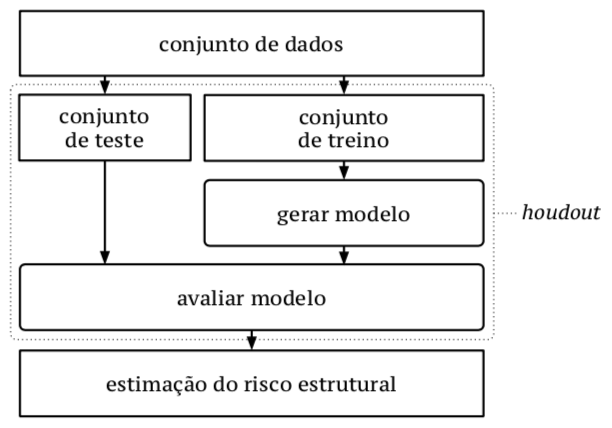
\includegraphics[width=.5\linewidth]{holdout.png}
    \begin{tikzpicture}[auto,
        block/.style = {rectangle, draw, fill=none, text width=8em, text centered, minimum height=2em}]
        % Place nodes
        \node [block, text width=15em] (dataset) {\scriptsize conjunto de dados};
        \node [block, node distance=1.8cm, below right of=dataset, xshift=0.15cm] (train) {\scriptsize conjunto de treinamento};
        \node [block, node distance=1.8cm, below left of=dataset, text width=6em, xshift=-0.6cm] (test) {\scriptsize conjunto de teste};
        \node [block, node distance=1.5cm, below of=train] (model) {\scriptsize gerar modelo};
        \node [block, node distance=4.25cm, text width=15em, below of=dataset] (evaluate) {\scriptsize avaliar modelo};
        \node [block, below of=evaluate, node distance=1.25cm, text width=15em] (risk) {\scriptsize estimação do risco estrutural};

        % Draw edges
        \draw[red, very thick, dotted, rounded corners] ($(test.north west)+(-0.2,0.2)$) rectangle ($(evaluate.south east)+(0.2,-0.2)$) node[text=black] at ($(model.east)+(1.2,0)$, 0) {\scriptsize \textit{holdout}};
        \path [line] ([xshift=14.2mm] dataset.south) -- (train.north);
        \path [line] ([xshift=-18.8mm] dataset.south) -- (test.north);
        \path [line] (train) -- (model);
        \path [line] (model.south) -- ([xshift=14.2mm] evaluate.north);
        \path [line] (test.south) -- ([xshift=-18.8mm] evaluate.north);
        \path [line] (evaluate) -- (risk);
    \end{tikzpicture}
    \begin{center}
        \makebox[\width]{Fonte: \citeonline{madson2017}.}
    \end{center}
\end{figure}

A técnica de validação cruzada \textit{k-fold} realiza uma divisão do conjunto total de dados em $k$ partes (subconjuntos) mutuamente excludentes de mesmo tamanho. Em seguida, um total de $k-1$ partes é utilizado no treinamento do algoritmo, enquanto a parte restante é utilizada para validação do modelo obtido. Este processo é realizado $k$ vezes, alternando de forma circular o $k$-ésimo conjunto utilizado para validação. Quando o processo é encerrado, computa-se o risco médio para os $k$ modelos, que é utilizado como estimação do risco estrutural. A Figura \ref{fig:k-fold} ilustra o processo descrito acima.

\begin{figure}[H]
    \caption{Uso do método \textit{k-fold} para estimação do risco empírico.}
    \label{fig:k-fold}
    \centering
    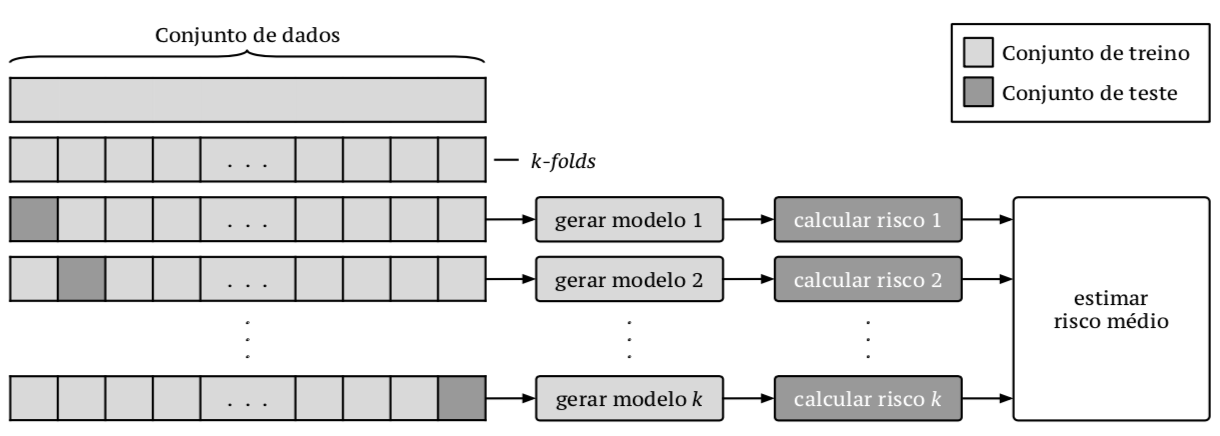
\includegraphics[width=\linewidth]{kfold.png}
    \begin{center}
        \makebox[\width]{Fonte: \citeonline{madson2017}.}
    \end{center}
\end{figure}

A realização de todos os experimentos deste trabalho utilizou uma combinação dos métodos \textit{holdout} e \textit{k-fold}. Primeiramente, o método \textit{holdout} realizou uma divisão onde 80\% dos dados foi utilizado para treinamento e os 20\% restantes para teste foi utilizado para estimação das métricas de desempenho, que para o caso específico de regressão são RMSE e tempo (total) médios. Em seguida, o método \textit{k-fold}, com 5 divisões ($k=5$), foi utilizado para definição da aptidão de cada indivíduo (\textit{kernel}), utilizando o conjunto de treinamento para tal divisão.

Existem ainda um conjunto de parâmetros relativos ao arcabouço de PG que precisa ser definido. A população inicial é criada utilizando o método \textit{ramped half-and-half} com faixa de profundidade $[2, 4]$. As probabilidades de uso dos operadores de cruzamento e mutação são 0.85 e 0.15, respectivamente. O método de seleção utilizado foi a seleção por torneio lexicográfico de tamanho 5. O tamanho da população foi definido em 30 indivíduos. Por fim, o número de gerações escolhido foi 30. A Tabela \ref{tab:pg-params} apresenta uma lista destes parâmetros e seus respectivos valores.

% Por último, o parâmetro de regularização foi fixado com valor $0.01$

\begin{table}[H]
    \caption{Resumo dos parâmetros utilizados nas realizações da PG.}
    \label{tab:pg-params}
    \begin{center}
        \begin{tabular}{l@{\hskip 18pt}l}
            \hline\noalign{\smallskip}
            \textbf{Parâmetro} & \textbf{Valor}\\
            \noalign{\smallskip}
            \hline
            \noalign{\smallskip}
            Número de gerações & 30 \\
            Tamanho da população & 30 \\
            Faixa de profundidade & $[2, 4]$ \\
            População inicial & \textit{ramped half-and-half} \\
            Método de seleção & \textit{lexicographic tournament} \\
            Tamanho do torneio & 5 \\
            Probabilidade de cruzamento & 0.85 \\
            Probabilidade de mutação & 0.15 \\
            \hline
        \end{tabular}
    \end{center}
    \begin{center}
        \makebox[\width]{Fonte: Autor.}
    \end{center}
\end{table}

\vspace*{-0.7cm}

Cada experimento foi realizado 30 vezes para cada par \textit{conjunto de dados/modelo} com base na seleção aleatória dos subconjuntos de treinamento e teste, com o parâmetro de regularização com valor fixo de $0.01$. As estimativas das métricas de avaliação foram definidas como uma média geral das 30 realizações.

\subsection{Comparação com modelos estado-da-arte}
Para fins de comparação de desempenho com o modelo proposto, são utilizados os seguintes modelos estado-da-arte: SVR, MLP e RBF. Especificamente para o SVR, foram utilizados os \textit{kernels} linear, polinomial e rbf. Para todos estes modelos, os hiperparâmetros foram obtidos utilizando uma modificação da metodologia do GKR: durante a validação cruzada de \textit{k-folds} é realizada uma busca em grade sobre uma faixa de valores dos hiperparâmetros. Para tornar a comparação mais justa, todos os modelos foram submetidos às mesmas divisões do método \textit{k-fold}, garantindo então que todos sejam submetidos às mesmas variações dos conjuntos de dados. O algoritmo de treinamento do SVR utilizado nos experimentos é o SMO \cite{platt1999}.

O hiperparâmetro do SVR com \textit{kernel} linear é apenas a constante de regularização \textit{C}, onde foi utilizado a faixa de valores em escala logarítmica $[10^{-3}, 10^3]$. Os outros \textit{kernels} (\textit{rbf} e polinomial) possuem dois hiperparâmetros, um deles sendo a constante $\gamma$ (com a mesma faixa de valores usada para o \textit{kernel} linear). Especificamente para o \textit{kernel} polinomial, foi utilizado a faixa de valores $[2, 4]$ para o grau do polinômio. Já para o SVR com \textit{kernel} rbf foi utilizada a faixa de valores em escala logarítmica $[10^{-3}, 10^3]$.

Para a rede neural MLP, o hiperparâmetro é o número de neurônios da camada oculta, em que a faixa de valores escolhida foi $[5, 25]$. O treinamento do MLP é realizado através do algoritmo de Levenberg-Marquardt \cite{hagan1994}. Já para a rede RBF \cite{powell1987}, há dois hiperparâmetros: o número de neurônios da camada oculta e a abertura da função gaussiana, $\sigma$. O número de neurônios da camada oculta tem faixa de valores em $[5, 25]$. A abertura da função gaussiana possui faixa de valores $[2^{-5}, 2^5]$.

\section{Resultados e Discussões} \label{sec:results}
Nesta seção são apresentados os resultados das simulações realizadas para avaliação da proposta deste trabalho. Para isso, o GKR, assim como SVR, MLP e RBF, são aplicados a diversos conjuntos de dados de natureza artificial e real, para problemas de regressão.

\subsection{Conjuntos de dados artificiais}
Para fins de análise do processo de treinamento, foram realizadas simulações utilizando conjuntos de dados artificiais de uma dimensão, uma vez que permite uma visualização das superfícies de decisão no plano cartesiano. Esta análise é importante, pois permite avaliar a capacidade de generalização dos modelos na representação dos dados, ou seja, a capacidade de aprendizado.

No primeiro grupo de experimentos deste trabalho foram utilizados apenas os seguintes modelos: GKR, MLP, RBF e SVR/RBF\footnote{É comum na literatura utilizar a nomenclatura \textit{regressor/algoritmo/kernel}; entretanto, como o algoritmo utilizado em todos os experimentos neste trabalho foi o SMO, a nomenclatura torna-se \textit{regressor/kernel}.}. Isso pode ser justificado pela pouca capacidade de generalização que os modelos SVR/LIN e SVR/POL apresentaram durante as simulações computacionais.

Na Figura \ref{fig:results-real-datasets} são apresentados os resultados obtidos para os seis conjuntos de dados artificiais. %A análise dos gráficos pode ser dividida em dois grupos: (\textit{i}) para funções com muitas 
Ao analisar os gráficos, percebe-se que os modelos GKR e SVR/RBF possuem superfícies bastante semelhantes, conseguindo representar bem os dados. Entre as redes neurais, a MLP é a mais eficiente na generalização dos dados, gerando superfícies mais flexíveis. Já a rede RBF não consegue obter o mesmo poder de generalização que a MLP, pois suas superfícies de decisão sempre seguem o formato da função gaussiana (formato de ``sino''). Nas Figuras \ref{fig:results-real-datasets-3} e \ref{fig:results-real-datasets-5}, entretanto, a rede RBF consegue uma boa representação, uma vez que o domínio de ambas as funções apresentam um formato parecido com partes da função gaussiana.

\begin{figure}[H]
    \caption{Superfícies de decisão geradas pelos modelos GKR, RBF, SVR/RBF e MLP para os conjuntos de dados artificiais.}
    \label{fig:results-real-datasets}
    \begin{subfigure}[b]{0.5\linewidth}
        \centering
        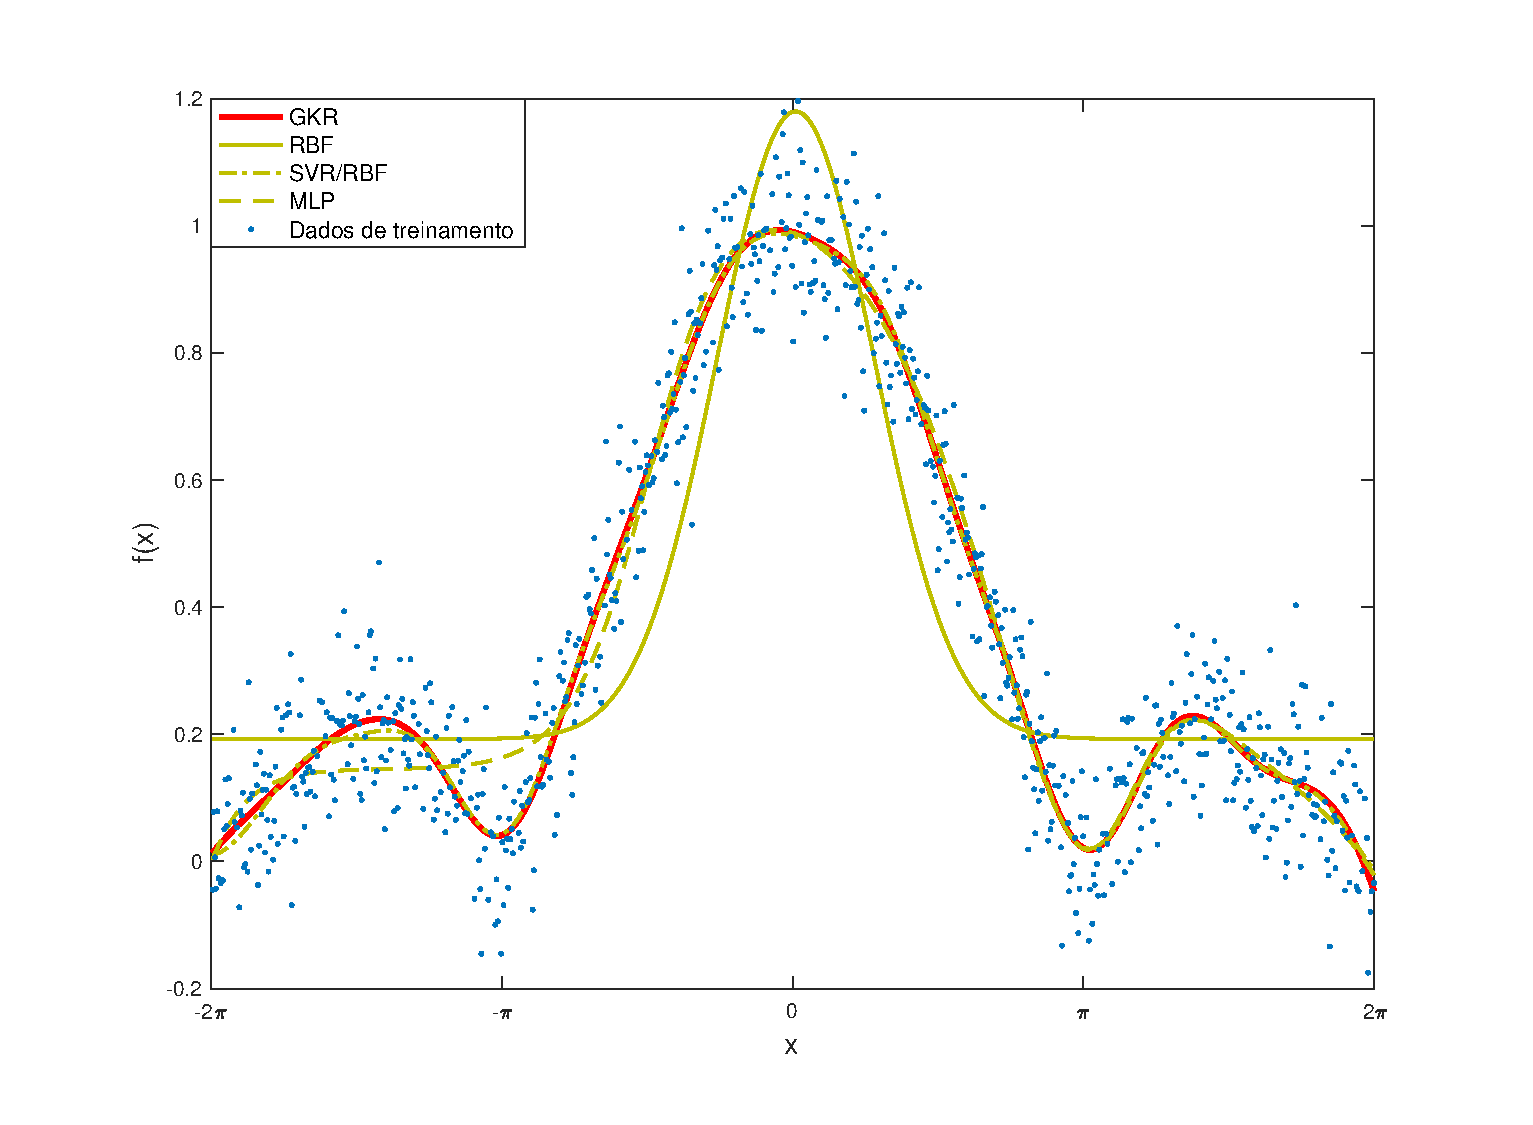
\includegraphics[width=\linewidth]{chapter4/art1.eps}
        \caption{Artificial 1} 
        \label{fig:results-real-datasets-1}
    \end{subfigure}%%
    \begin{subfigure}[b]{0.5\linewidth}
        \centering
        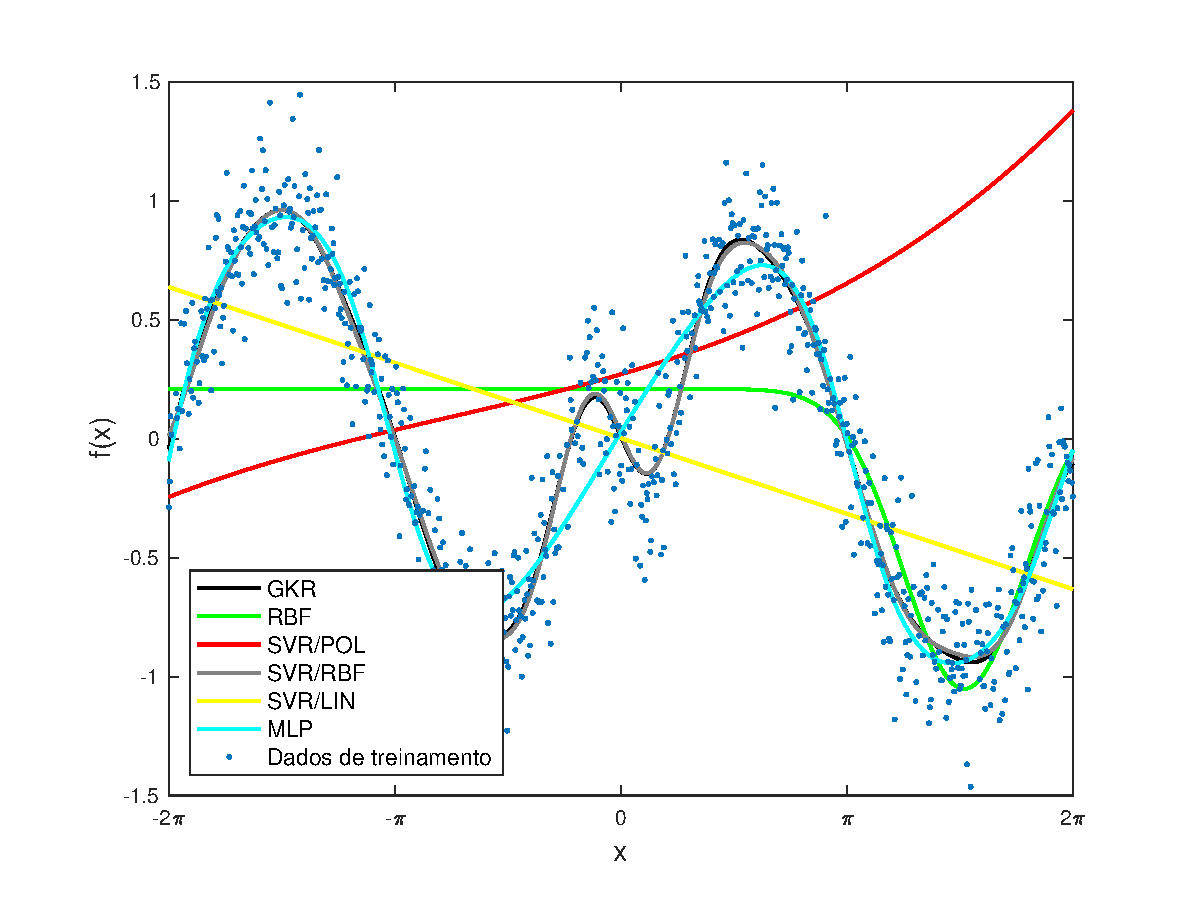
\includegraphics[width=\linewidth]{chapter4/art2.eps}
        \caption{Artificial 2}
        \label{fig:results-real-datasets-2}
    \end{subfigure}
    \begin{subfigure}[b]{0.5\linewidth}
        \centering
        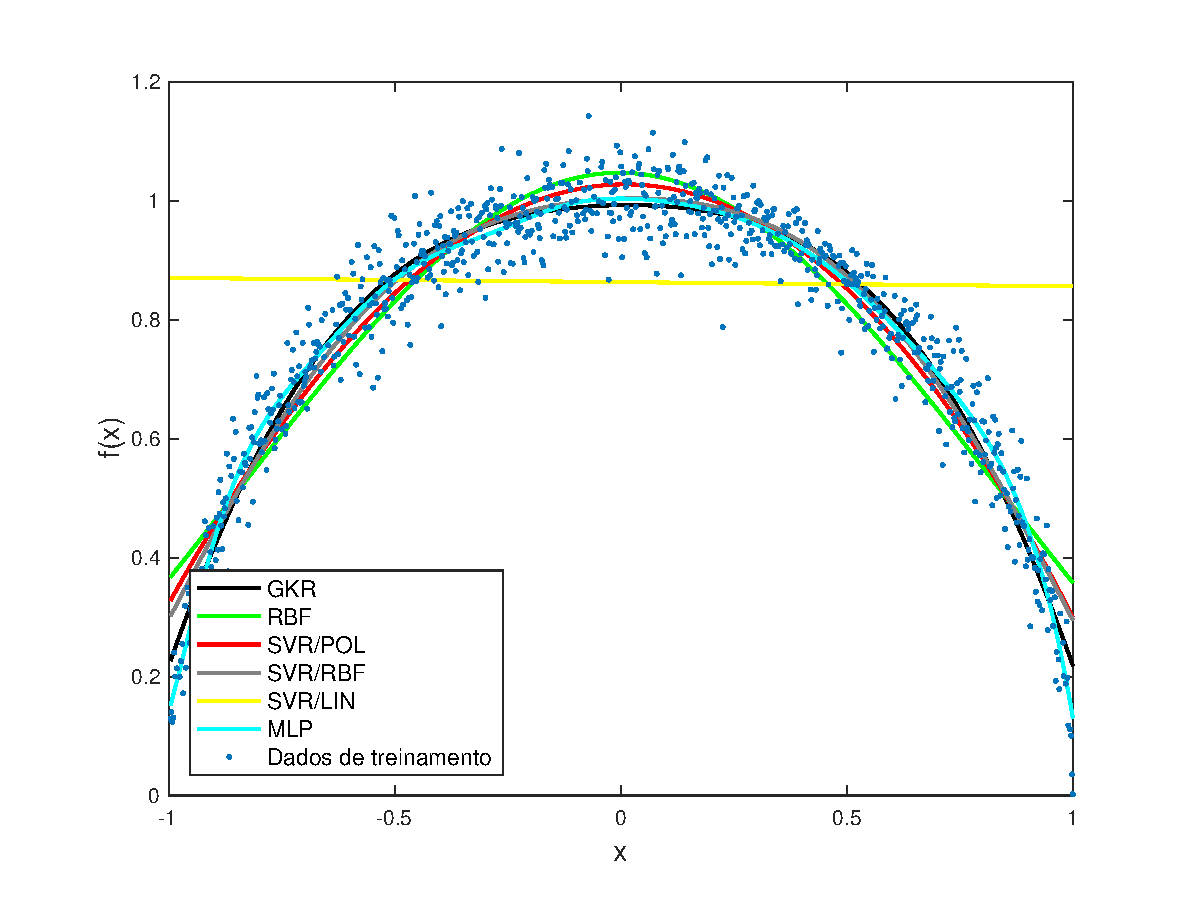
\includegraphics[width=\linewidth]{chapter4/art3.eps}
        \caption{Artificial 3}
        \label{fig:results-real-datasets-3}
    \end{subfigure}%%
    \begin{subfigure}[b]{0.5\linewidth}
        \centering
        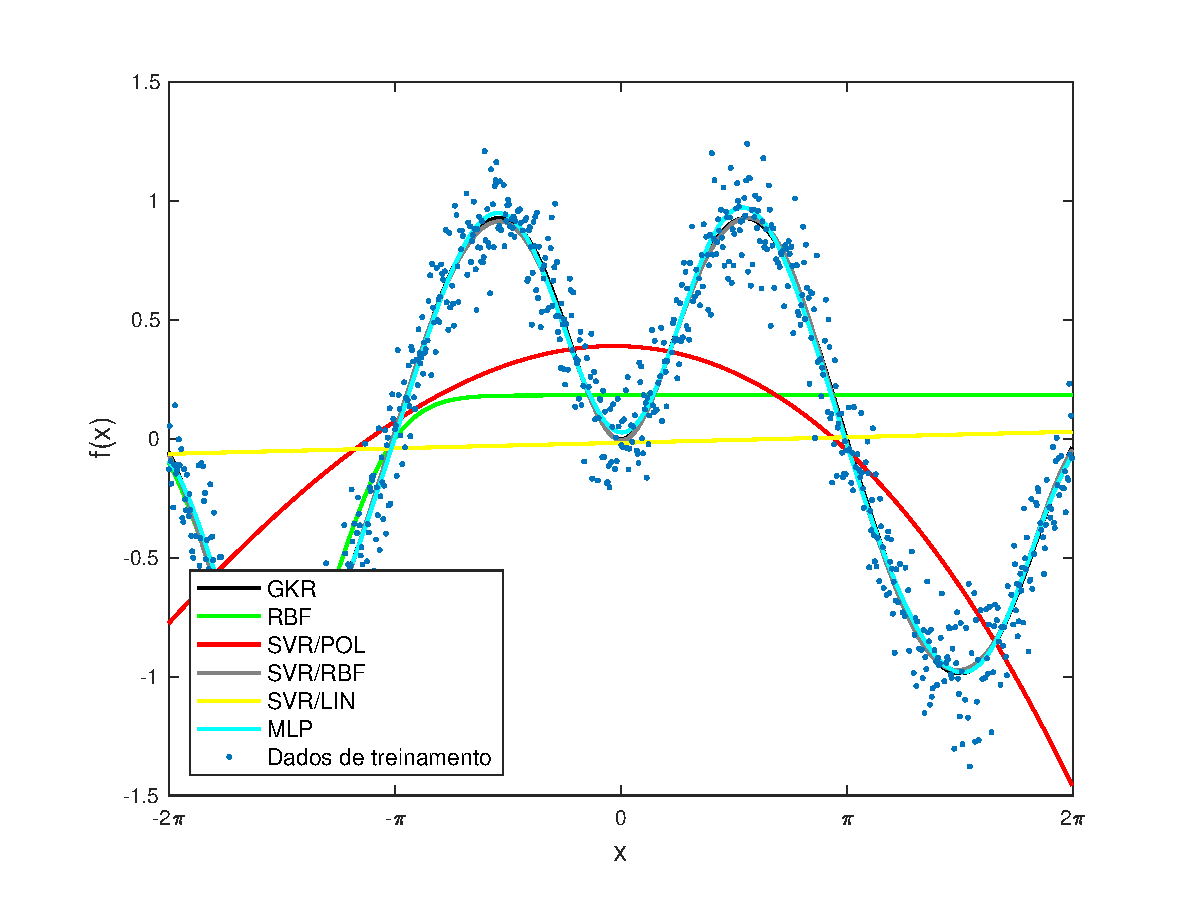
\includegraphics[width=\linewidth]{chapter4/art4.eps}
        \caption{Artificial 4}
        \label{fig:results-real-datasets-4}
    \end{subfigure}
    \begin{subfigure}[b]{0.5\linewidth}
        \centering
        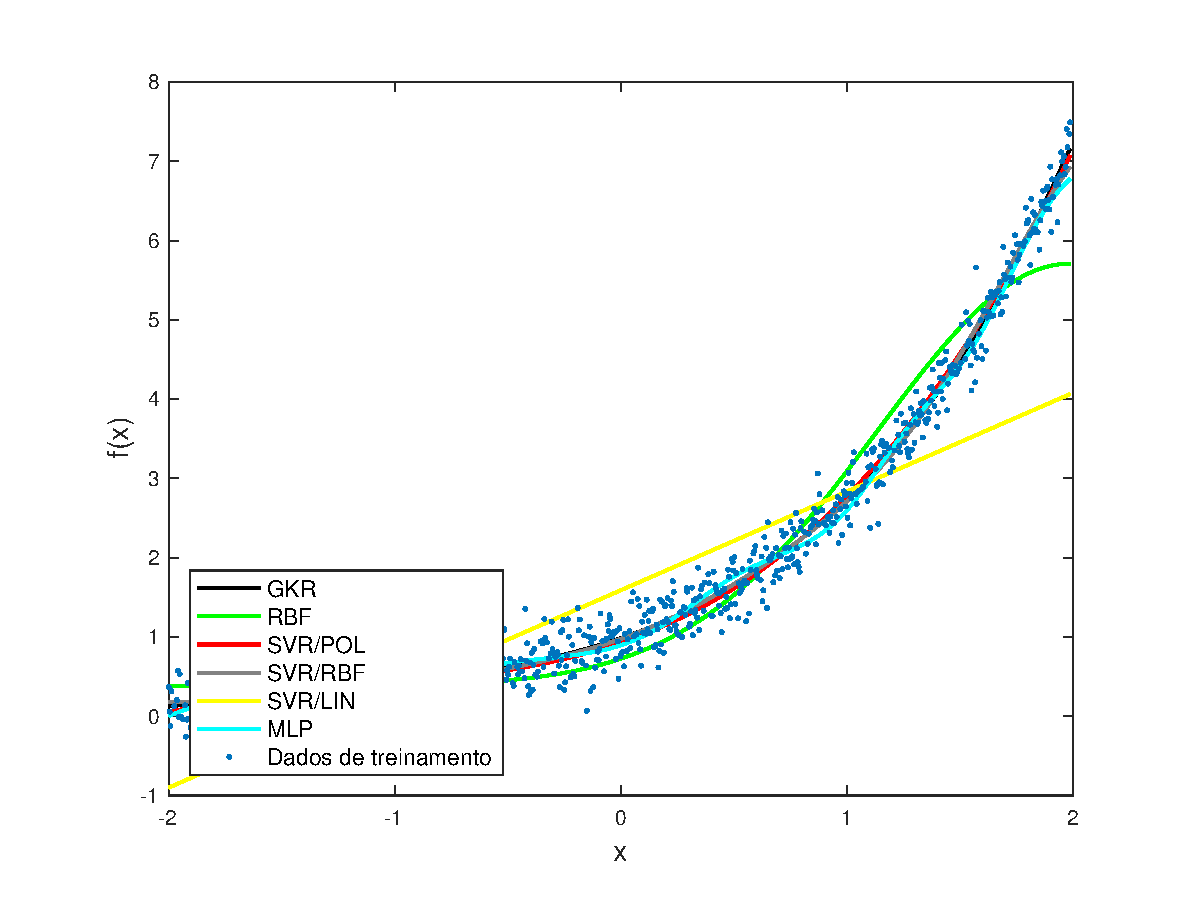
\includegraphics[width=\linewidth]{chapter4/art5.eps}
        \caption{Artificial 5}
        \label{fig:results-real-datasets-5}
    \end{subfigure}%%
    \begin{subfigure}[b]{0.5\linewidth}
        \centering
        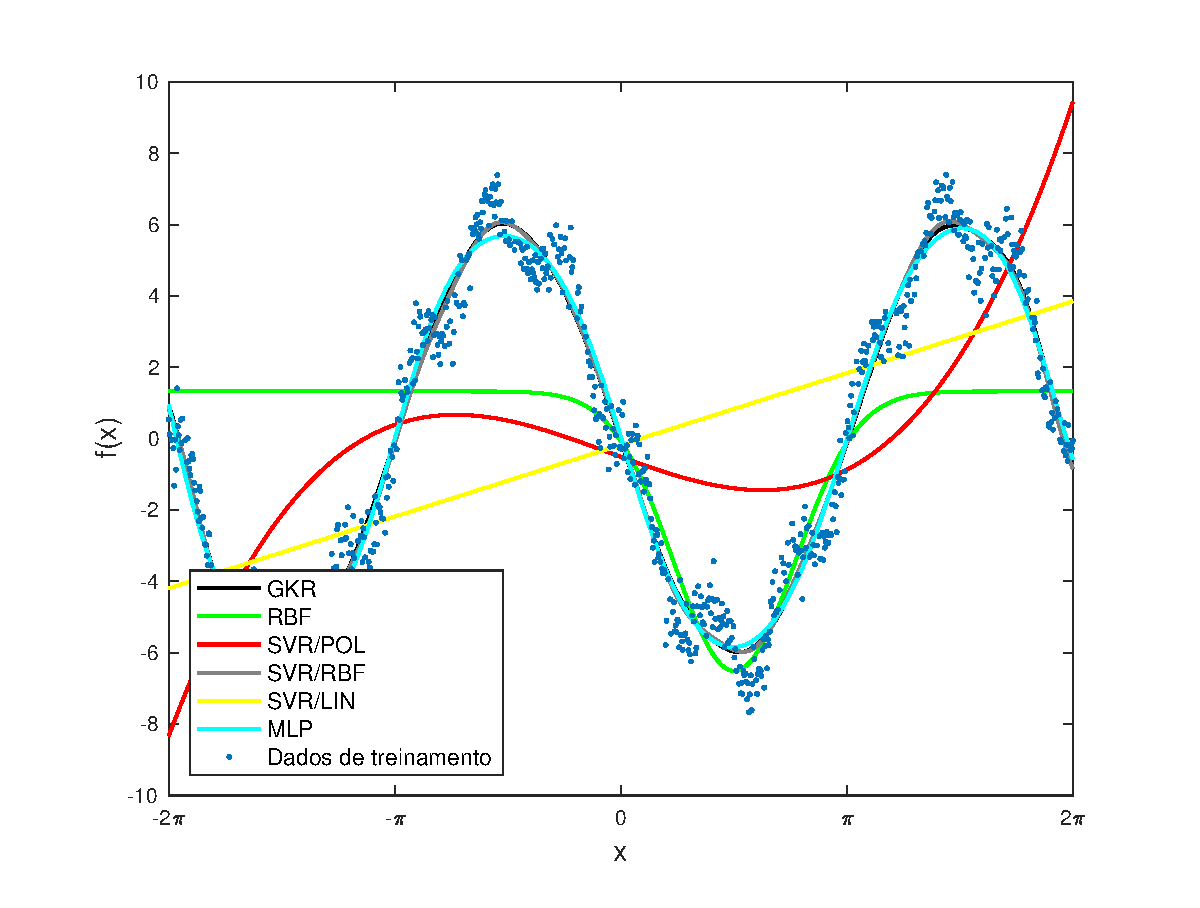
\includegraphics[width=\linewidth]{chapter4/art6.eps}
        \caption{Artificial 6}
        \label{fig:results-real-datasets-6}
    \end{subfigure} 
    \centering \makebox[\width]{Fonte: Autor.}
\end{figure}

\subsection{Conjuntos de dados reais}
O segundo grupo de experimentos tem como finalidade avaliar o desempenho do modelo GKR em problemas do mundo real, e compará-lo com o desempenho de modelos estado-da-arte. Para tal, as seguintes métricas serão analisadas: (\textit{i}) o desempenho das funções de \textit{kernel} será analisado através do valor de aptidão médio ao longo das gerações; (\textit{ii}) RMSE (média e desvio padrão); (\textit{iii}) tempo total (treinamento e teste) médio.

As Figuras \ref{fig:results-fitbygen1} e \ref{fig:results-fitbygen2} apresentam os resultados relativos aos conjuntos de dados reais. De modo geral, ao analisar ambas as figuras, percebe-se que a capacidade de representação dos dados vai se tornando cada vez melhor ao longo do processo de evolução. A partir disso pode-se confirmar que o algoritmo GKR consegue realizar a evolução das funções de \textit{kernel} de forma eficiente.

Um fator importante que precisa ser ressaltado é a influência que a natureza estocástica da PG exerce nos valores médios de aptidão a cada geração. De acordo com \citeonline{poli2008}, o processo de aprendizado de um sistema baseado em PG ocorre nas primeiras gerações\footnote{Os autores ainda afirmam que este é um dos motivos de que, de modo geral, o número de gerações de uma realização de PG é tipicamente inferior ou igual a 50.}. Portanto, é comum encontrar partes dos melhores indivíduos das primeiras gerações ao longo do processo de evolução. Portanto, a partir do crescimento do valor de aptidão médio ao longo das gerações, percebe-se que as funções de \textit{kernel} são candidatas equivalentes à solução ideal de cada problema (embora o modo em que a PG chega à essas funções é estocástico). Para a grande parte dos problemas, são poucos os decaimentos do valor de aptidão médio durante o processo de evolução. Entretanto, para problemas tais como \textit{Auto MPG}, \textit{Diabetes} e \textit{Servo Moto} há uma variação maior no valor de aptidão médio. Embora não seja um fator que chegue a causar descrédito ao GKR, pois o valor de aptidão médio permanece em faixas muito estritas (com mudanças na terceira casa decimal), serve para perceber duas situações: (\textit{i}) o conjunto de dados pode não representar bem o problema (ou seja, o problema pode sofrer de mal-condicionamento); (\textit{ii}) as funções de \textit{kernel} geradas durantes as realizações acabam não sendo candidatas equivalentes à solução do problema, o que acarreta no decaimento da aptidão média.

Para analisar a variabilidade do valor de aptidão média, pode ser realiza uma análise sobre a Tabela \ref{tab:results-rmse}. De modo geral, para todas os problemas reais utilizados neste trabalho, o desvio padrão dos modelos de regressão foi baixo -- com exceção da rede RBF, que para os problemas \textit{Diabetes} e \textit{Sleep}, obteve desvios padrões muito grandes. O fato de o RMSE não possuir muita variabilidade ao longo das 30 realizações permite inferir que o modelo GKR, assim como os modelos estado-da-arte, possui uma robustez grande a diversos problemas de regressão. Outro ponto a ser destacado é a capacidade de gerar diferentes funções de \textit{kernel} que conseguem adaptar-se à aleatoriedade dos conjuntos de treinamento e da própria natureza da PG; este fato permite inferir que o GKR consegue representar bem os dados que são apresentados a ele e construir \textit{kernels} adequados para cada situação.

Também é válido analisar o custo computacional e o tempo total necessário para realização dos modelos. Como era esperado (e já discutido brevemente no Capítulo \ref{chapter:kernel-methods}), o custo computacional do modelo KRR é da ordem $\mathcal{O}(n^3 + n^2p)$, onde $n$ é o número de padrões do conjunto e $p$ é a dimensionalidade dos padrões. Em conjunto com o arcabouço de PG, o tempo médio dispendido para treinamento e teste foi muito alto (inclusive maior que todos os modelos estado-da-arte). Porém, a justificativa para tais custos reside na validação cruzada de \textit{k-folds} que é realizada para cada indivíduo de cada população ao longo das gerações. Dessa forma, é de se esperar que o tempo necessário seja maior que dos outros modelos utilizados neste trabalho.

% Por fim, é feito uma análise entre os modelos SVR e KRR. Modelos como o SVR (e SVMs, de modo geral), advém da teoria do aprendizado estatístico. Uma característica importante do SVR é que ele consegue minimizar uma combinação do risco empírico e um termo de regularização responsável pela suavização da solução \cite{daniel2017}. O KRR possui uma formulação mais simples que o SVR. A principal diferença encontradas são a função de perda (\textit{ridge} para o KRR, \textit{\epsilon-insensitive} para o SVR)

\begin{figure}[H]
    \caption{Gráficos dos valores de aptidão médios ao longo das gerações (Parte 1).}
    \label{fig:results-fitbygen1}
    \begin{subfigure}[b]{0.5\linewidth}
        \centering
        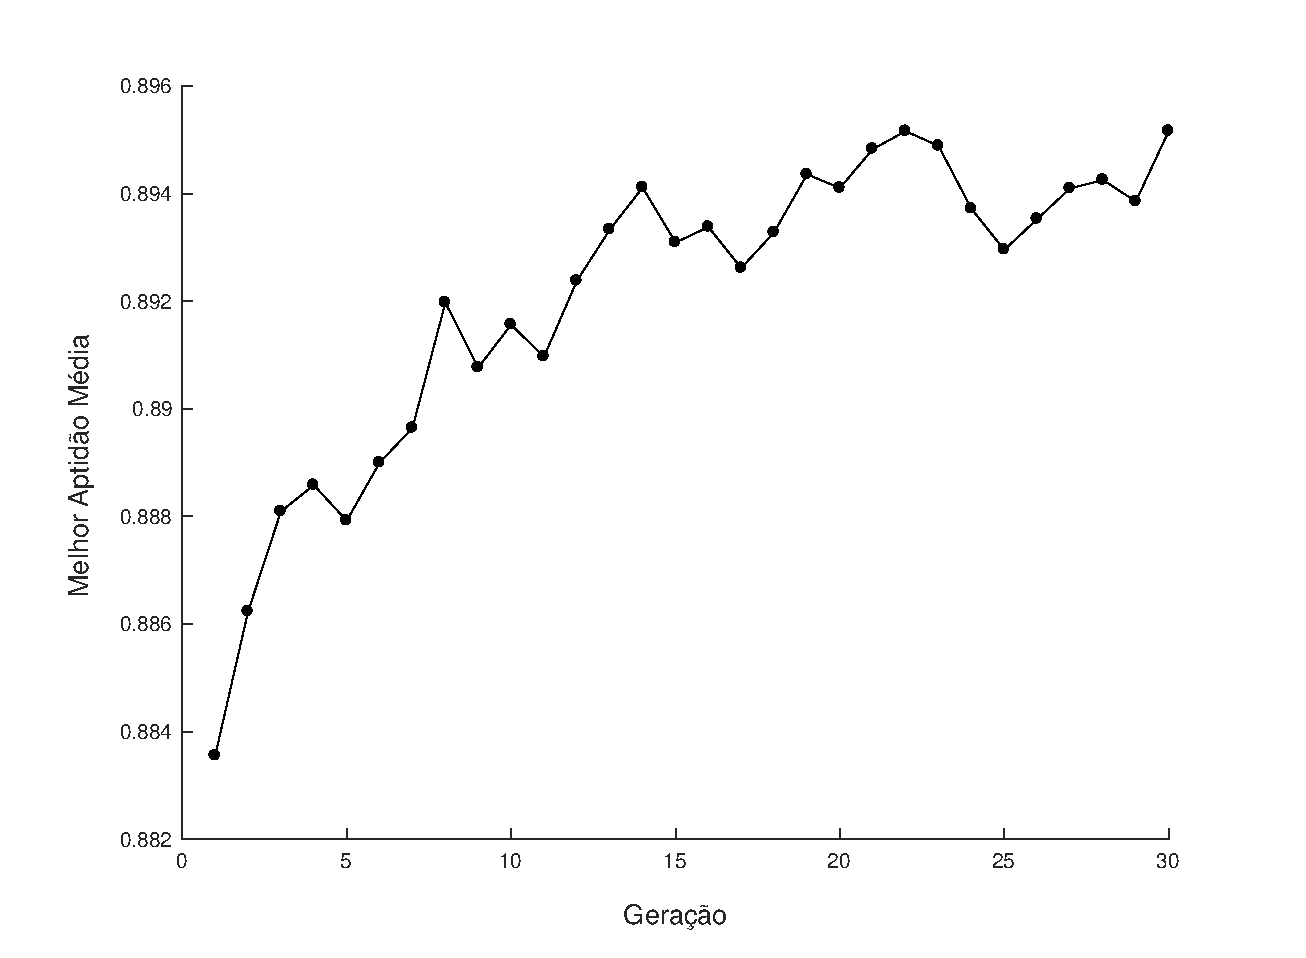
\includegraphics[width=\linewidth]{chapter4/air-pollution.eps}
        \caption{\textit{Air Pollution}} 
        \label{fig7:a}
    \end{subfigure}%%
    \begin{subfigure}[b]{0.5\linewidth}
        \centering
        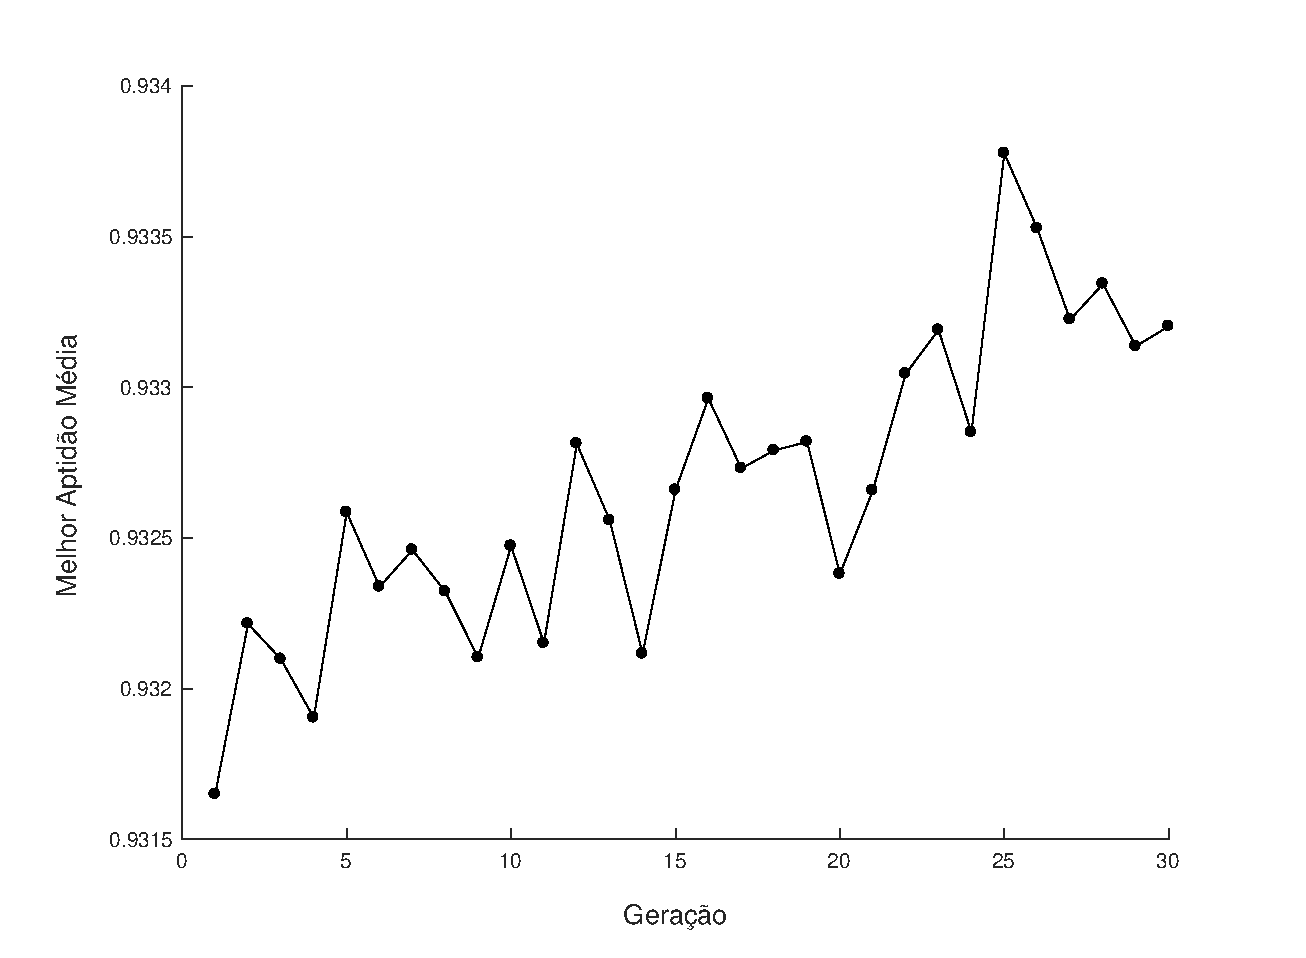
\includegraphics[width=\linewidth]{chapter4/auto-mpg.eps}
        \caption{\textit{Auto MPG}}
        \label{fig7:b}
    \end{subfigure}
    \begin{subfigure}[b]{0.5\linewidth}
        \centering
        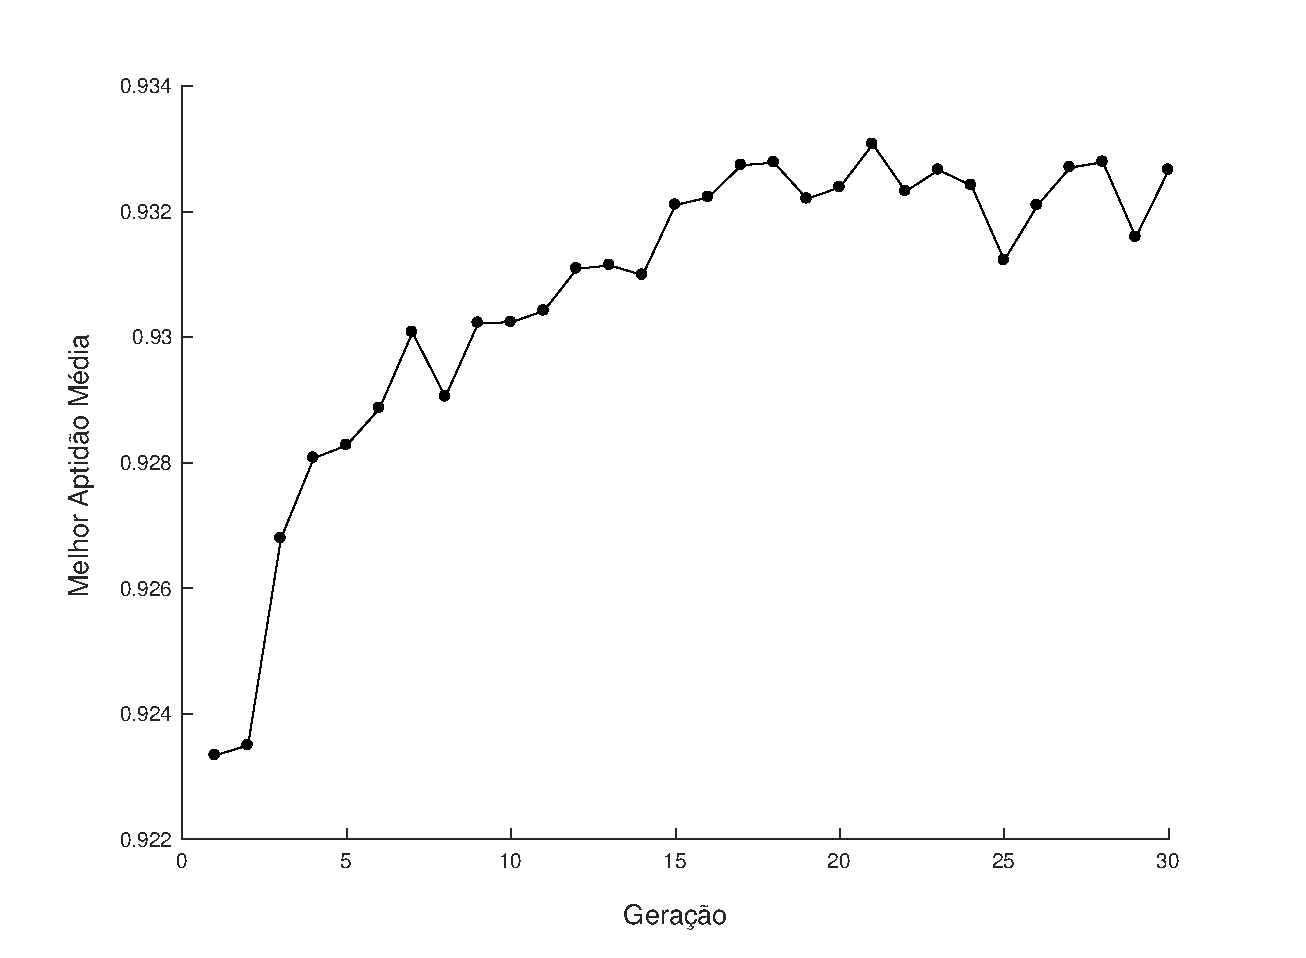
\includegraphics[width=\linewidth]{chapter4/auto-price.eps}
        \caption{\textit{Auto Price}}
        \label{fig7:c}
    \end{subfigure}%%
    \begin{subfigure}[b]{0.5\linewidth}
        \centering
        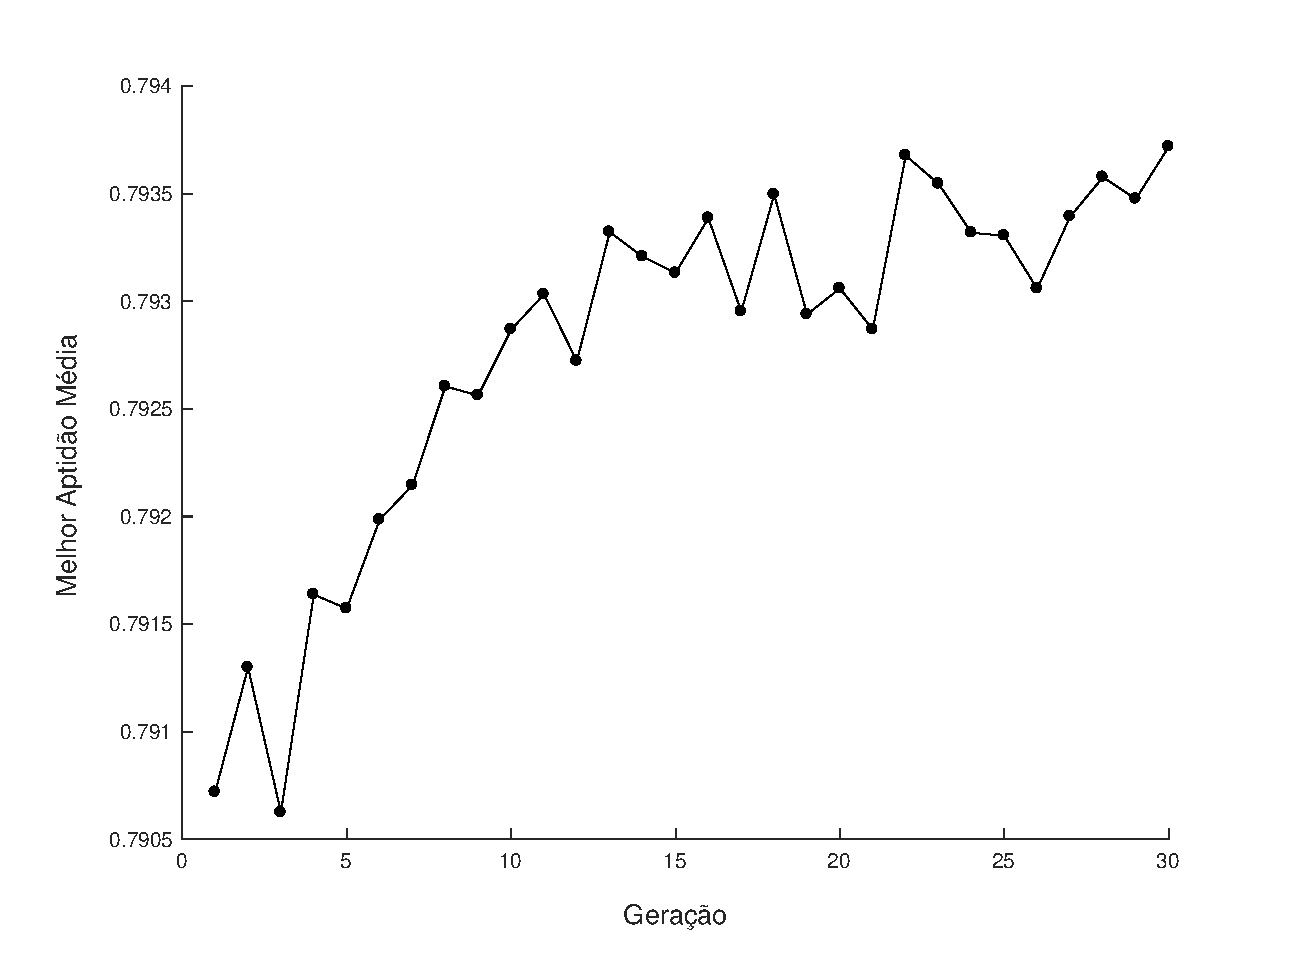
\includegraphics[width=\linewidth]{chapter4/breast-cancer.eps}
        \caption{\textit{Wisconsin Prognostic Breast Cancer}}
        \label{fig7:d}
    \end{subfigure}
    \begin{subfigure}[b]{0.5\linewidth}
        \centering
        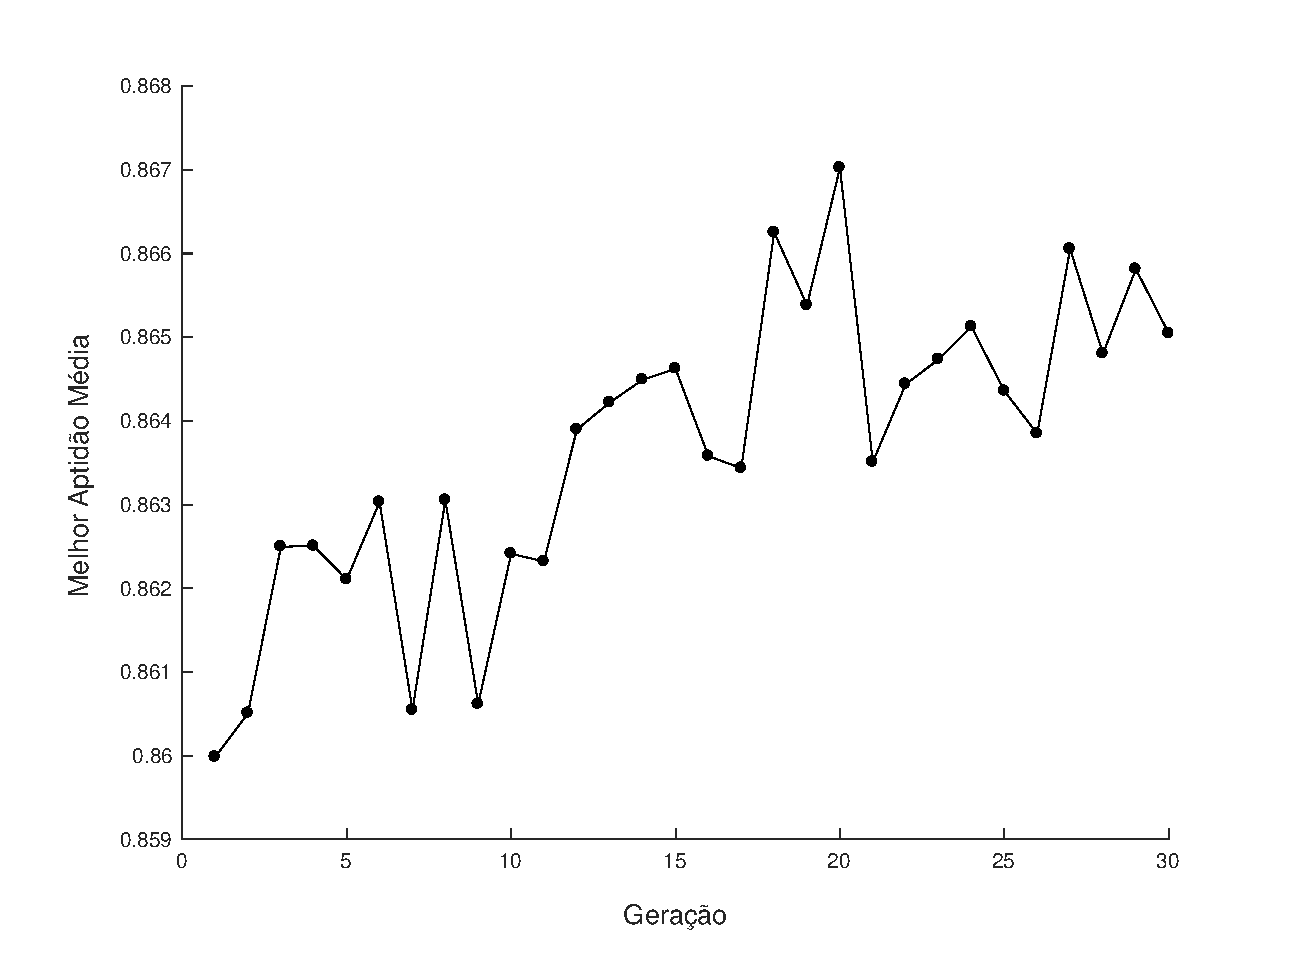
\includegraphics[width=\linewidth]{chapter4/diabetes.eps}
        \caption{\textit{Diabetes}}
        \label{fig7:e}
    \end{subfigure}%%
    \begin{subfigure}[b]{0.5\linewidth}
        \centering
        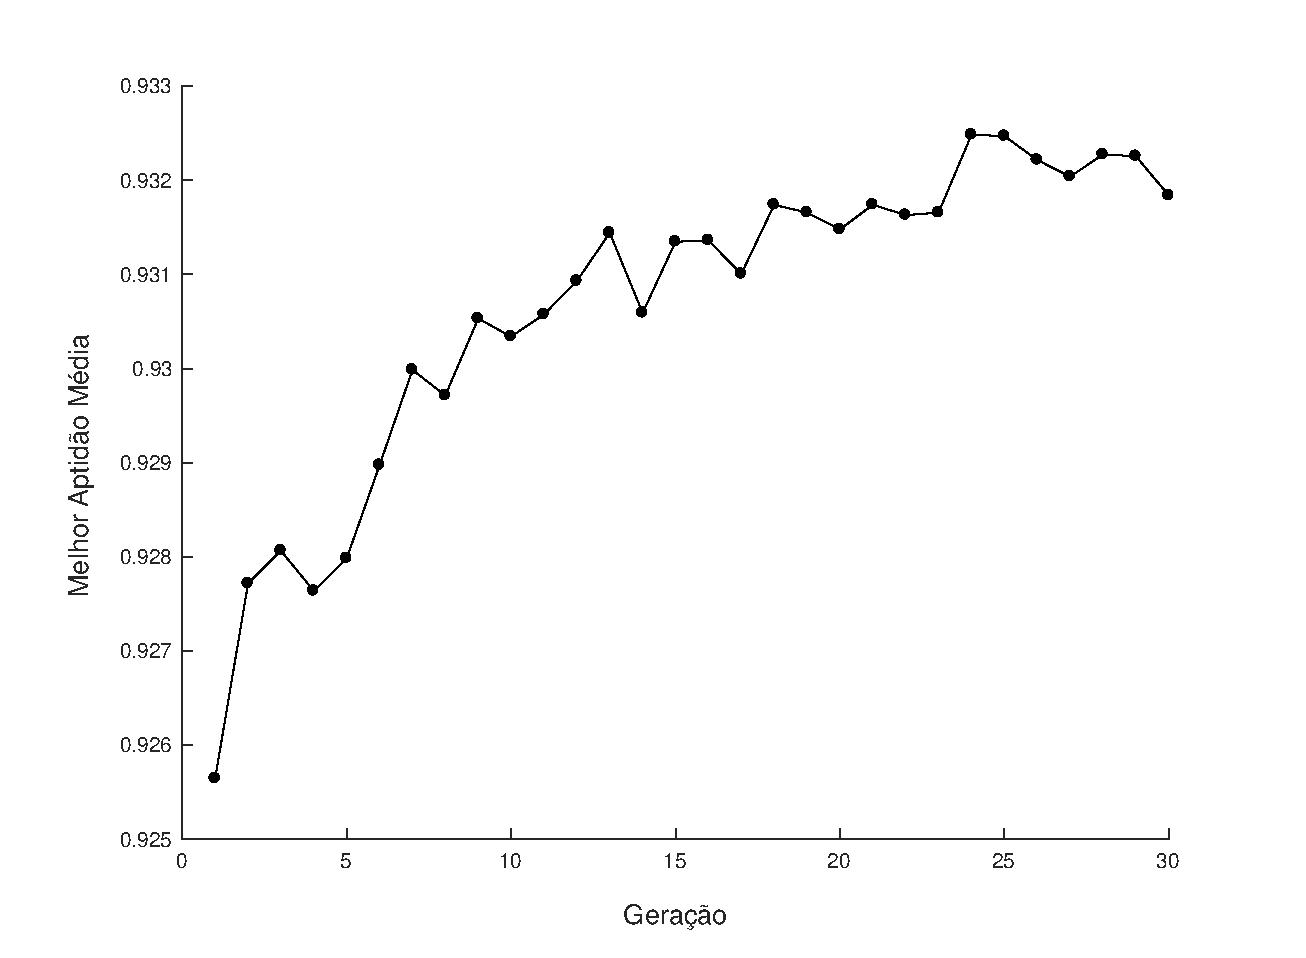
\includegraphics[width=\linewidth]{chapter4/housing.eps}
        \caption{\textit{Boston Housing}}
        \label{fig7:f} 
    \end{subfigure} 
    \centering \makebox[\width]{Fonte: Autor.}
\end{figure}
\begin{figure}[H]
    \caption{Gráficos dos valores de aptidão médios ao longo das gerações (Parte 2).}
    \label{fig:results-fitbygen2}
    \begin{subfigure}[b]{0.5\linewidth}
        \centering
        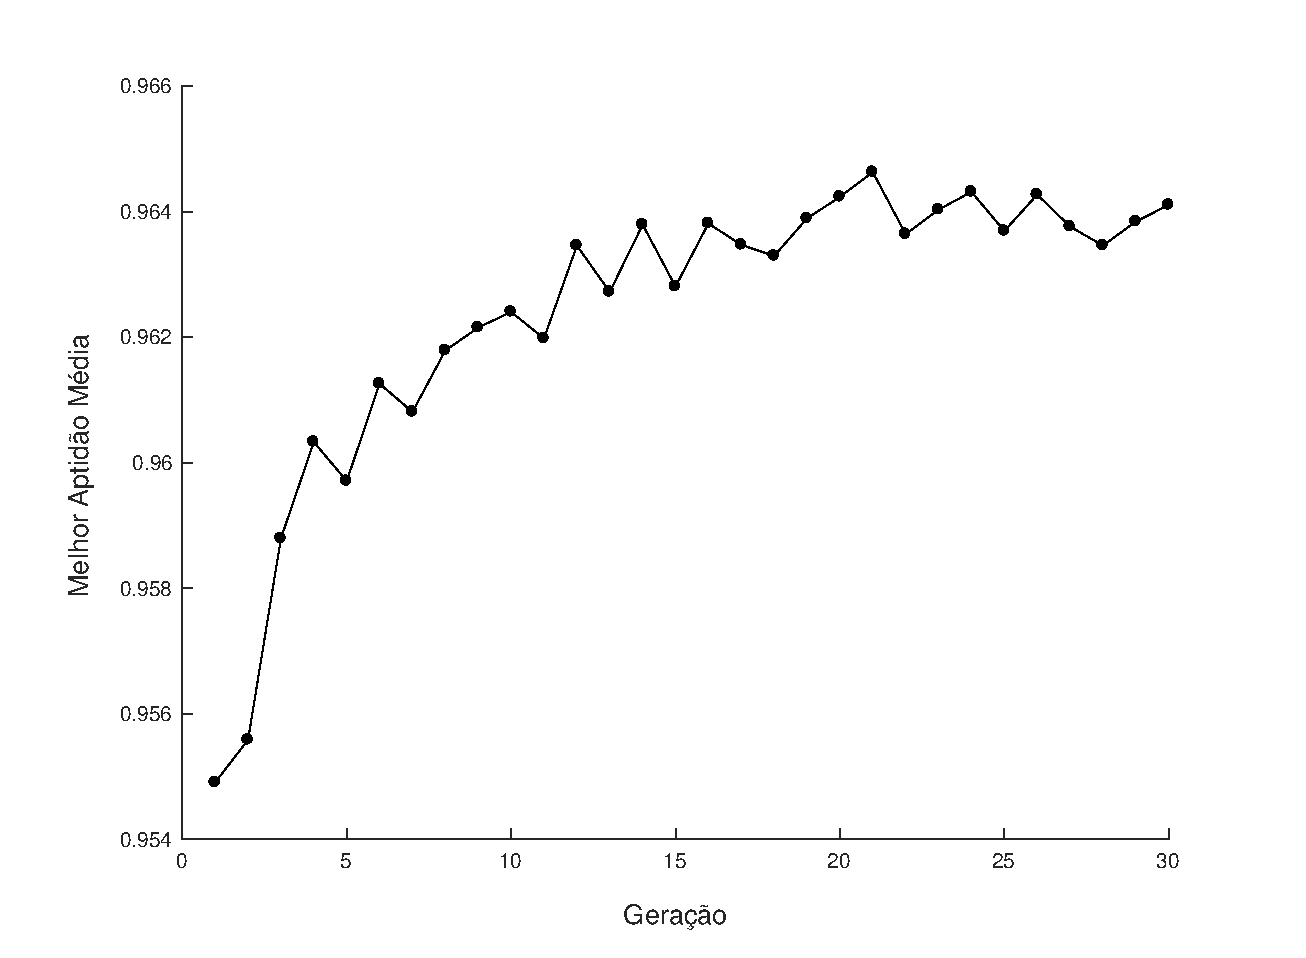
\includegraphics[width=\linewidth]{chapter4/machine-cpu.eps}
        \caption{\textit{Computer Hardware}} 
        \label{fig8:a}
    \end{subfigure}%%
    \begin{subfigure}[b]{0.5\linewidth}
        \centering
        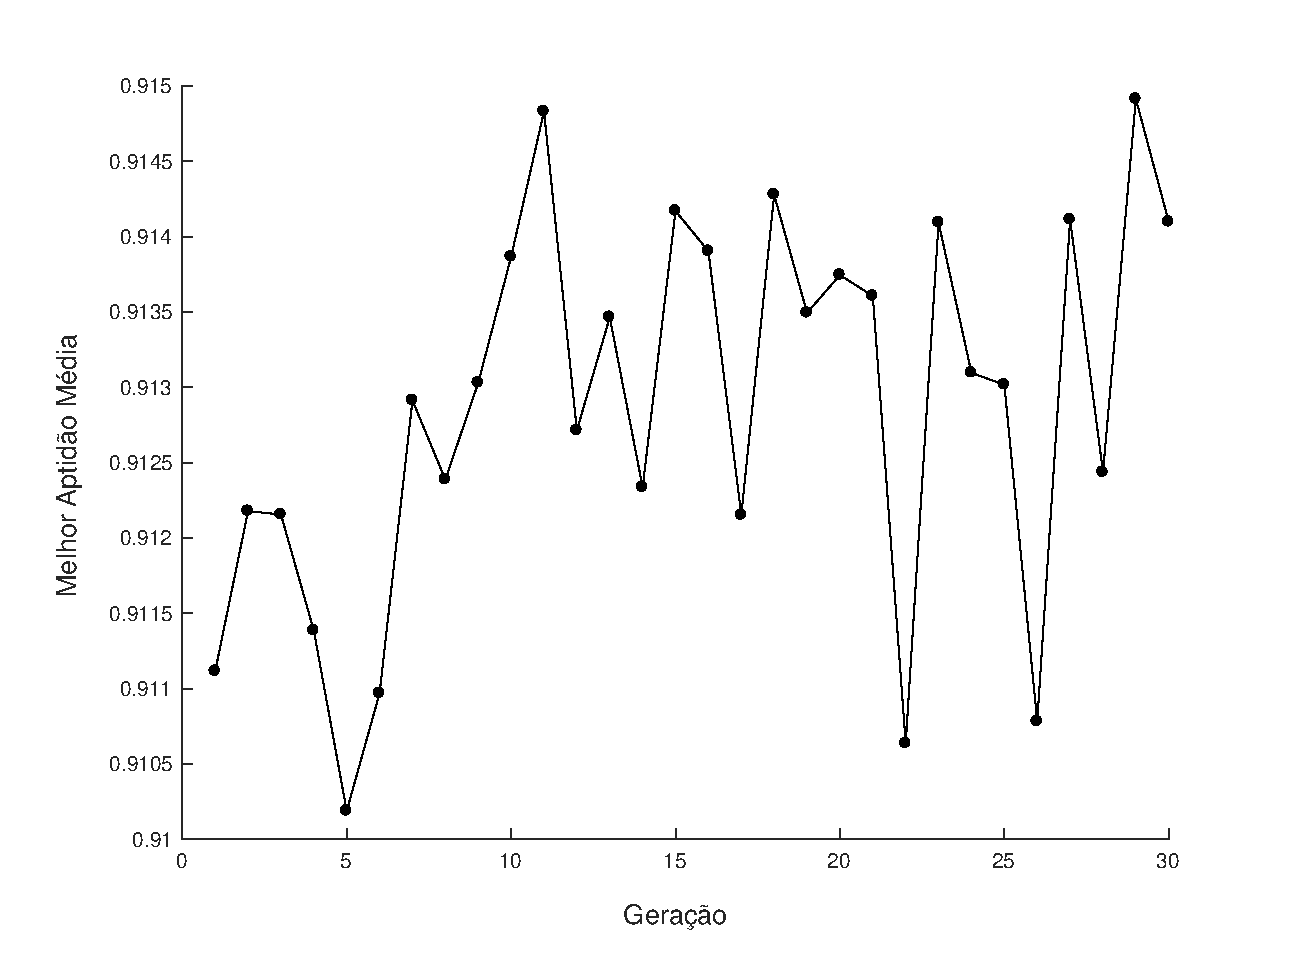
\includegraphics[width=\linewidth]{chapter4/servo.eps}
        \caption{\textit{Servo Motor}}
        \label{fig8:b}
    \end{subfigure}
    \begin{subfigure}[b]{0.5\linewidth}
        \centering
        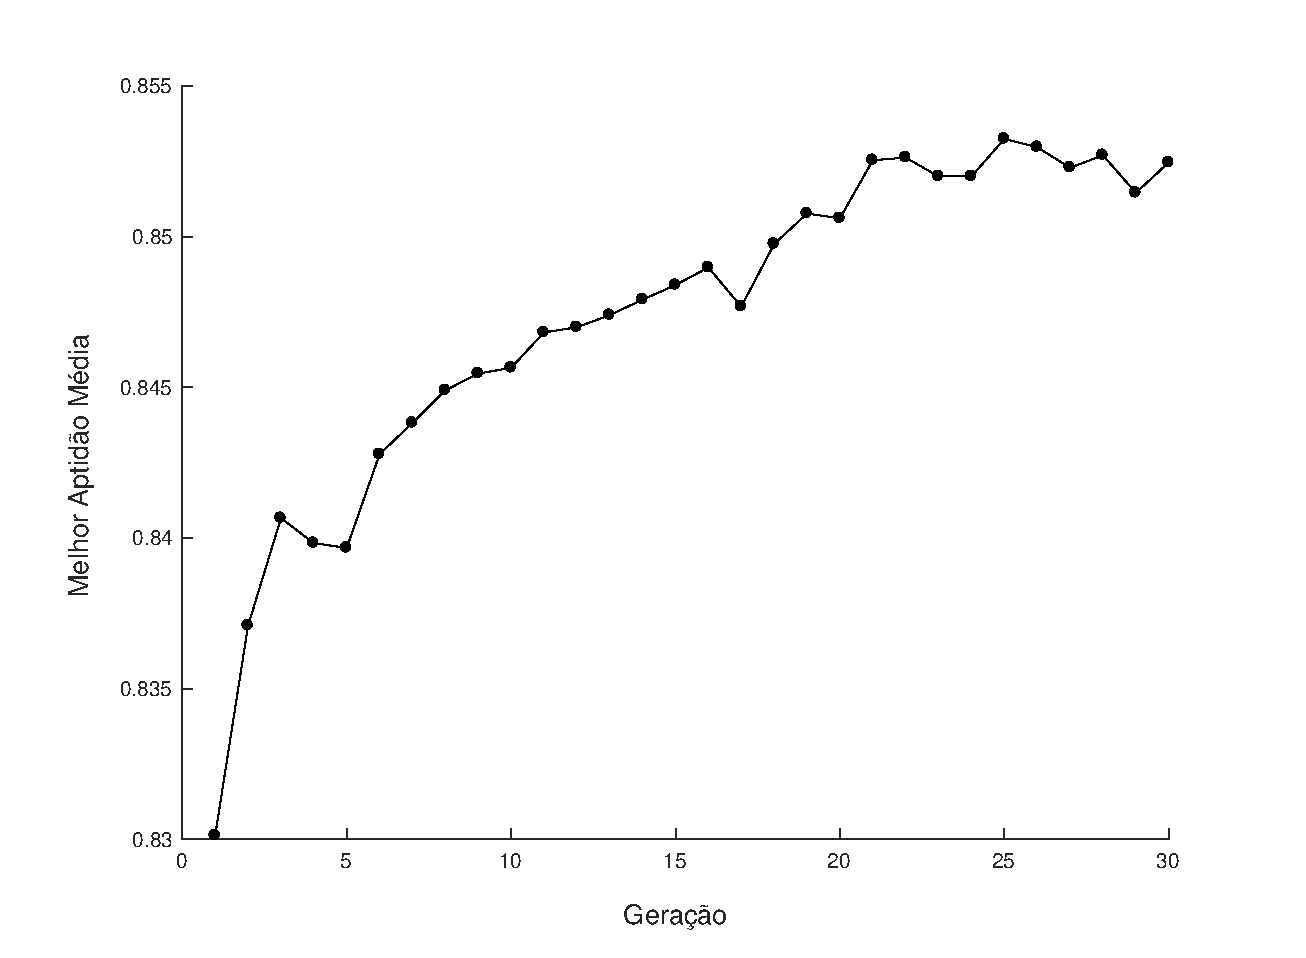
\includegraphics[width=\linewidth]{chapter4/sleep.eps}
        \caption{\textit{Sleep}}
        \label{fig8:c}
    \end{subfigure}%%
    \begin{subfigure}[b]{0.5\linewidth}
        \centering
        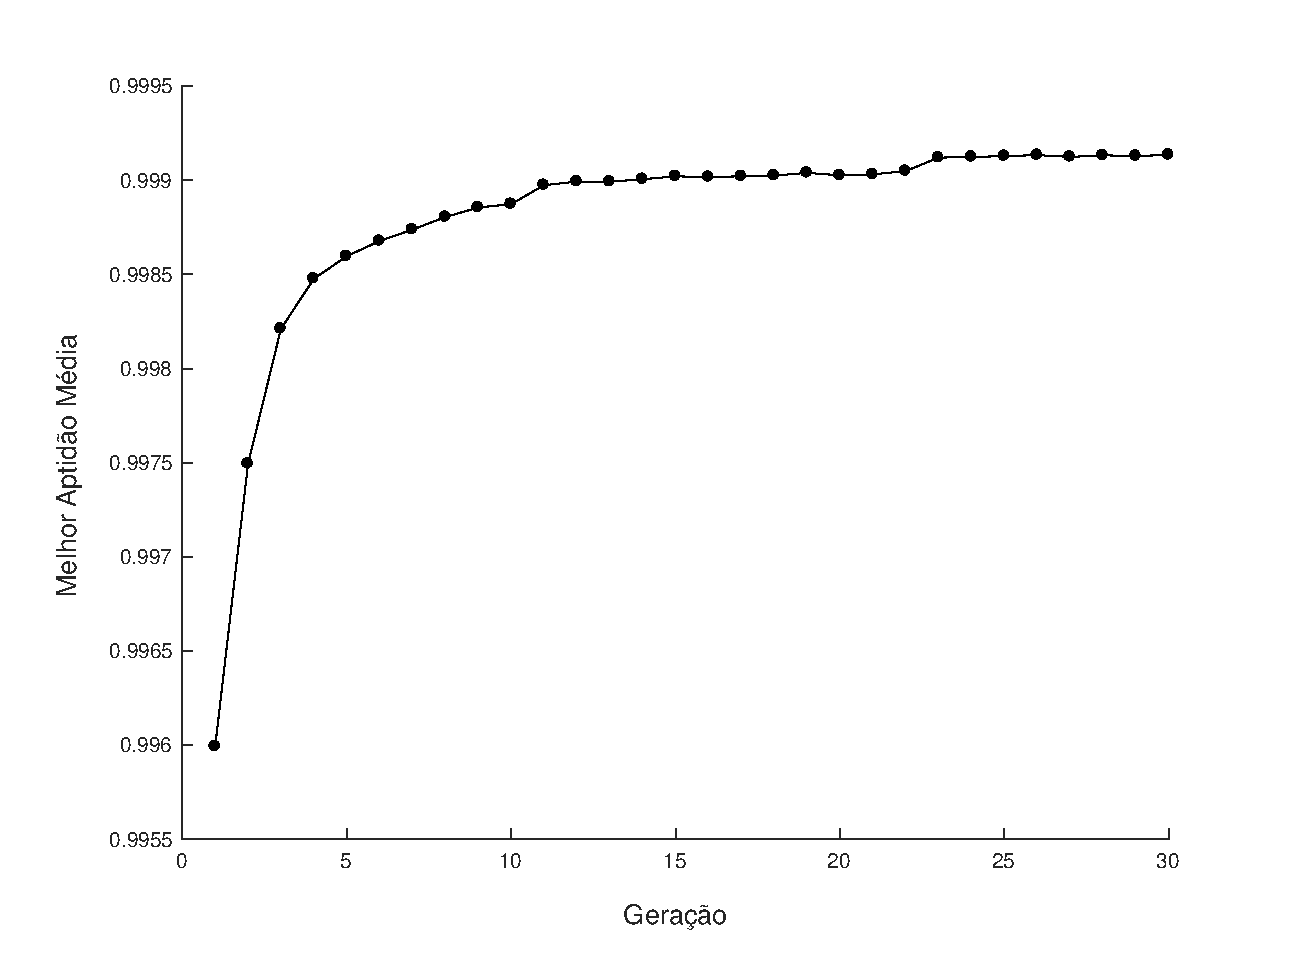
\includegraphics[width=\linewidth]{chapter4/spiritwt.eps}
        \caption{\textit{Spirituos Liquors}}
        \label{fig8:f}
    \end{subfigure}
    \begin{subfigure}[b]{0.5\linewidth}
        \centering
        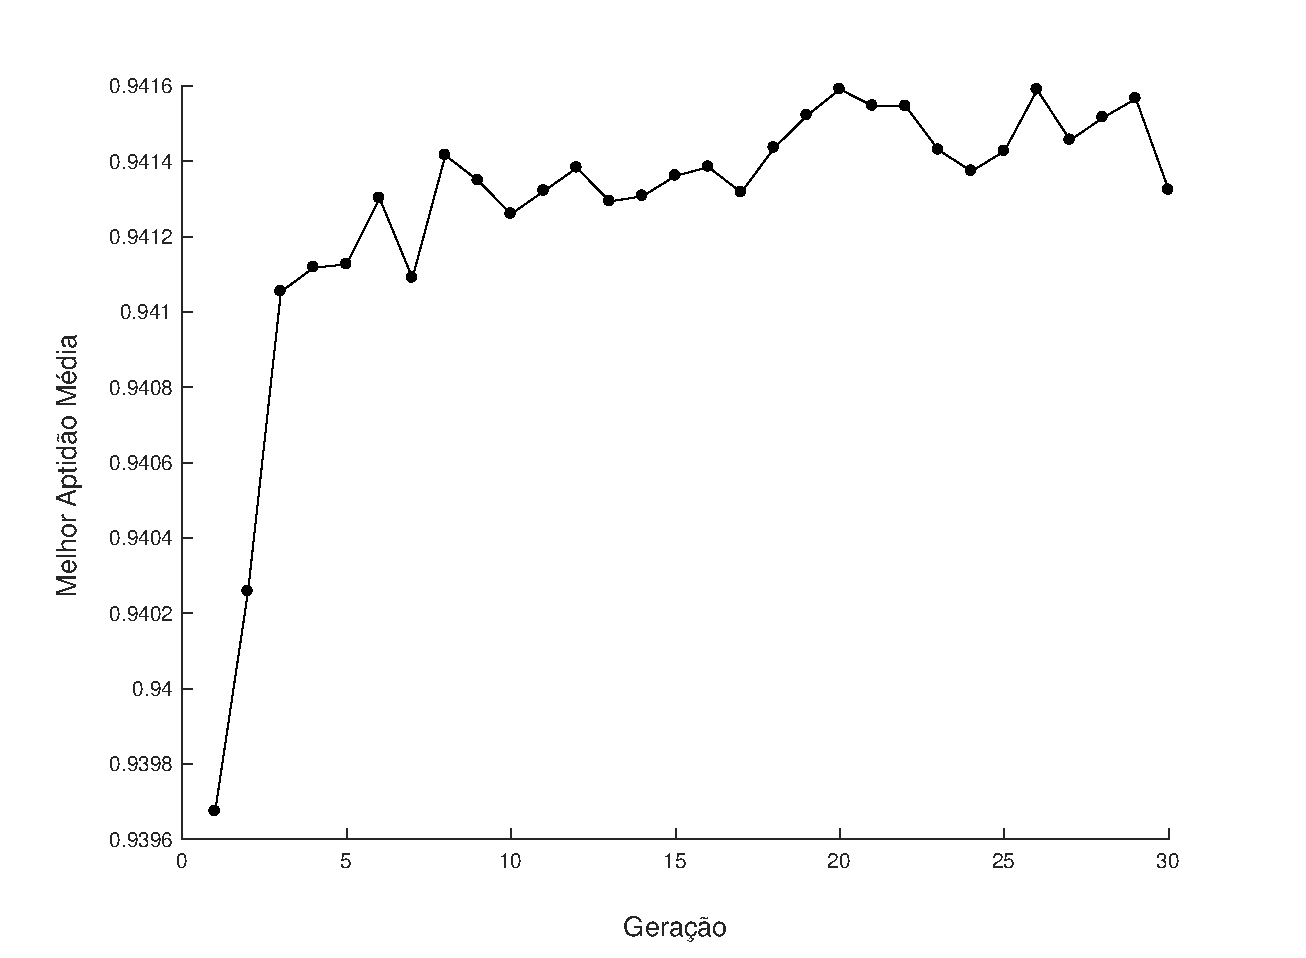
\includegraphics[width=\linewidth]{chapter4/stocks.eps}
        \caption{\textit{Stock Prices}}
        \label{fig8:d}
    \end{subfigure}%%
    \begin{subfigure}[b]{0.5\linewidth}
        \centering
        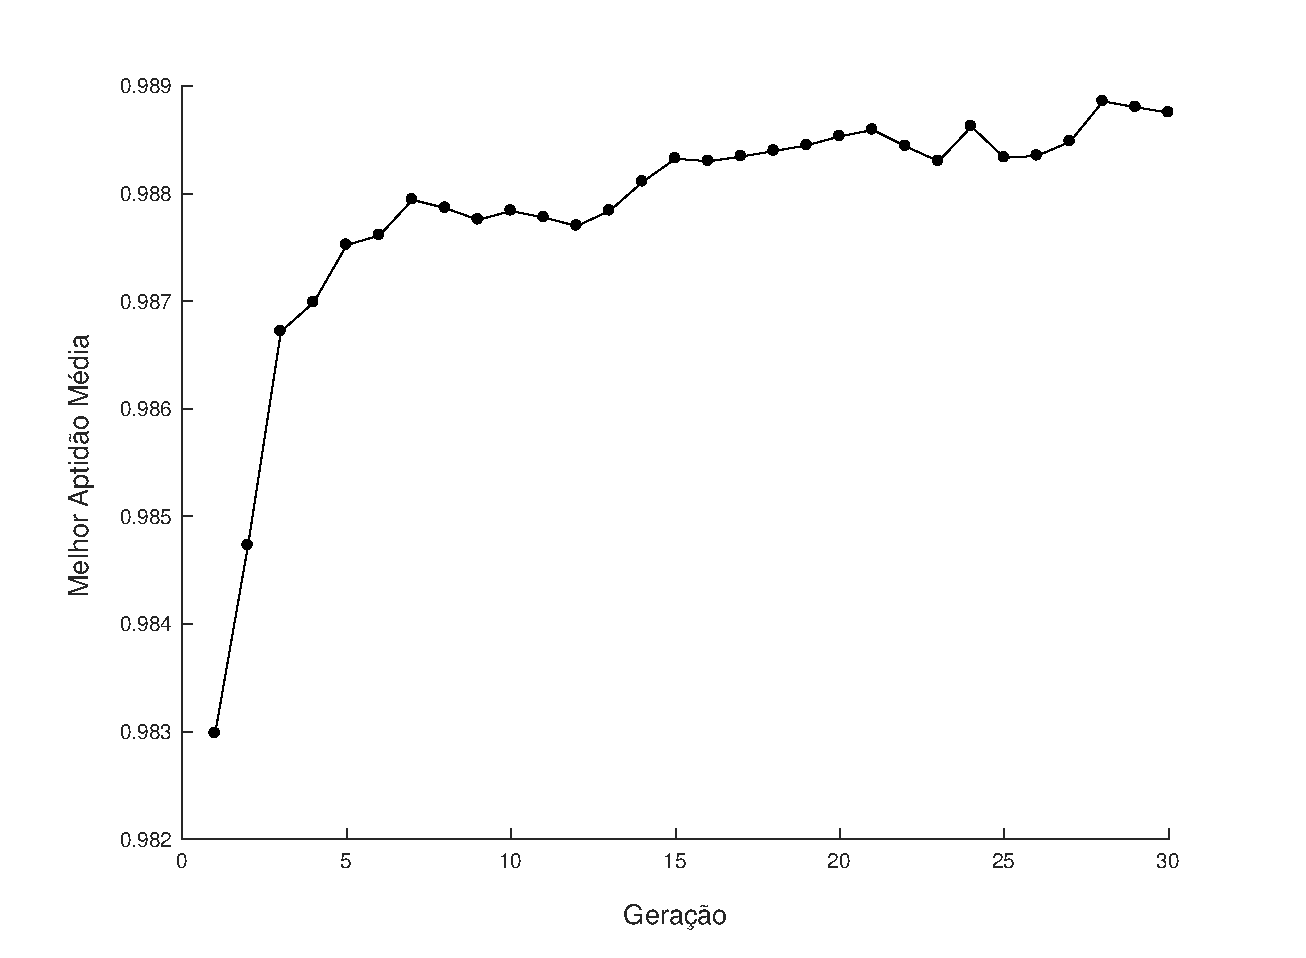
\includegraphics[width=\linewidth]{chapter4/yacht.eps}
        \caption{\textit{Yacht Hydrodynamics}}
        \label{fig8:e}
    \end{subfigure}
    \centering \makebox[\width]{Fonte: Autor.}
\end{figure}

\begin{landscape}
    \begin{table}
        \centering
        \caption{RMSE e tempo total (treinamento e teste) médios de todas as técnicas sobre os conjuntos de dados reais.}
        \label{tab:results-rmse}
        \begin{tabular}{l|l|c@{\hskip 5pt}c@{\hskip 5pt}c@{\hskip 5pt}c@{\hskip 5pt}c@{\hskip 5pt}c}
            \toprule
            \multicolumn{2}{l}{\textbf{Conjunto de dados}} & \textbf{GKR} & \textbf{SVR/LIN} & \textbf{SVR/RBF} & \textbf{SVR/POL} & \textbf{MLP} & \textbf{RBF} \\
            \midrule
            \multirow{2}{*}{APOL}   & RMSE & $0.1360 \pm 0.0331$ & $\textbf{0.1246} \pm \textbf{0.0264}$ & $0.1294 \pm 0.0248$ & $0.1578 \pm 0.0498$ & $0.1612 \pm 0.0367$ & $0.1913 \pm 0.0649$ \\
                                    & Tempo (s) & $469652.30$ & $249.06$ & $20191.93$ & $37230.50$ & $17948.53$ & $16839.90$ \\
            \midrule
            \multirow{2}{*}{AMPG}   & RMSE & $0.0748 \pm 0.0089$ & $0.0945 \pm 0.0095$ & $\textbf{0.0727} \pm \textbf{0.0091}$ & $0.0762 \pm 0.0099$ & $0.0959 \pm 0.0073$ & $0.2663 \pm 0.0943$ \\
                                    & Tempo (s) & $601425.77$ & $172.23$ & $18398.40$ & $54114.76$ & $18983.53$ & $218956.50$ \\
            \midrule
            \multirow{2}{*}{APRI}   & RMSE & $\textbf{0.0773} \pm \textbf{0.0232}$ & $0.0901 \pm 0.0185$ & $0.0909 \pm 0.0244$ & $0.0812 \pm 0.0185$ & $0.0963 \pm 0.0149$ & $0.0838 \pm 0.0215$ \\
                                    & Tempo (s) & $299075.60$ & $66.63$ & $11864.96$ & $25424.90$ & $11142.83$ & $15466.16$ \\
            \midrule
            \multirow{2}{*}{BHOU}   & RMSE & $\textbf{0.0705} \pm \textbf{0.0134}$ & $0.1096 \pm 0.0152$ & $0.0929 \pm 0.0179$ & $0.0766 \pm 0.0178$ & $0.1114 \pm 0.0110$ & $0.1066 \pm 0.0213$ \\
                                    & Tempo (s) & $381618.90$ & $70.30$ & $24801.80$ & $82692.87$ & $12411.93$ & $107767.97$ \\
            \midrule
            \multirow{2}{*}{CHAR}   & RMSE & $0.0524 \pm 0.0373$ & $0.0588 \pm 0.0322$ & $0.0693 \pm 0.0433$ & $0.0575 \pm 0.0346$ & $0.0694 \pm 0.0216$ & $\textbf{0.0514} \pm \textbf{0.0232}$ \\
                                    & Tempo (s) & $296862.33$ & $63.70$ & $11621.53$ & $24732.67$ & $10452.77$ & $6508.03$ \\
            \midrule
            \multirow{2}{*}{DIAB}   & RMSE & $0.1904 \pm 0.0570$ & $\textbf{0.1681} \pm \textbf{0.0383}$ & $0.1748 \pm 0.0402$ & $0.1742 \pm 0.0395$ & $0.1738 \pm 0.0464$ & $1.4968 \pm 1.9164$ \\
                                    & Tempo (s) & $430191.17$ & $198.07$ & $26038.67$ & $42552.50$ & $18907.00$ & $20731.70$ \\
            \midrule
            \multirow{2}{*}{SERV}   & RMSE & $\textbf{0.0870} \pm \textbf{0.0177}$ & $0.1911 \pm 0.0376$ & $0.1212 \pm 0.0422$ & $0.0926 \pm 0.0295$ & $0.1662 \pm 0.0179$ & $0.1759 \pm 0.1761$ \\
                                    & Tempo (s) & $583503.90$ & $109.13$ & $20633.30$ & $48024.23$ & $17055.33$ & $56257.00$ \\
            \midrule
            \multirow{2}{*}{SLEE}   & RMSE & $0.1896 \pm 0.0507$ & $0.1822 \pm 0.0315$ & $0.1922 \pm 0.0298$ & $\textbf{0.1782} \pm \textbf{0.0333}$ & $0.2629 \pm 0.1579$ & $18.7917 \pm 44.4962$ \\
                                    & Tempo (s) & $397893.73$ & $178.13$ & $20251.43$ & $39408.90$ & $18640.97$ & $17441.23$ \\
            \midrule
            \multirow{2}{*}{SPIR}   & RMSE & $\textbf{0.0008} \pm \textbf{0.0005}$ & $0.0496 \pm 0.0039$ & $0.0180 \pm 0.0030$ & $0.0192 \pm 0.0011$ & $0.0667 \pm 0.0020$ & $0.0244 \pm 0.0029$ \\
                                    & Tempo (s) & $982922.37$ & $191.03$ & $17347.23$ & $44298.63$ & $80656.60$ & $9519.30$ \\
            \midrule
            \multirow{2}{*}{STPR}   & RMSE & $\textbf{0.0262} \pm \textbf{0.0015}$ & $0.0847 \pm 0.0057$ & $0.0277 \pm 0.0020$ & $0.0311 \pm 0.0018$ & $0.0899 \pm 0.0045$ & $0.0361 \pm 0.0024$ \\
                                    & Tempo (s) & $671482.47$ & $140.93$ & $13440.30$ & $382495.63$ & $17045.13$ & $64897.67$ \\
            \midrule
            \multirow{2}{*}{YAHY}   & RMSE & $\textbf{0.0098} \pm \textbf{0.0020}$ & $0.1714 \pm 0.0221$ & $0.1181 \pm 0.0194$ & $0.0202 \pm 0.0030$ & $0.1483 \pm 0.00103$ & $0.0314 \pm 0.0074$ \\
                                    & Tempo (s) & $541210.30$ & $322.77$ & $38270.83$ & $169372.80$ & $26527.77$ & $11744.00$ \\
            \midrule
            \multirow{2}{*}{WPBC}   & RMSE & $\textbf{0.2558} \pm \textbf{0.0170}$ & $0.2629 \pm 0.0235$ & $0.2636 \pm 0.0250$ & $0.3335 \pm 0.0432$ & $0.2823 \pm 0.0300$ & $0.5227 \pm 0.1855$ \\
                                    & Tempo (s) & $467865.40$ & $208.70$ & $24975.87$ & $48350.63$ & $37693.87$ & $71121.93$ \\
            \bottomrule
        \end{tabular}
        \begin{center}
            \makebox[\width]{Fonte: Autor.}
        \end{center}
    \end{table}
\end{landscape}

\chapter{Conclusões e Trabalhos Futuros} \label{chapter:conclusions}

A popularidade dos modelos lineares deve-se a dois fatores: uma formulação matemática simples e propriedades bastante exploradas. Entretanto, a capacidade de generalização destes modelos é limitada, não sendo eficiente em solucionar muitos problemas do mundo real. A não-linearidade característica de tais problemas requer a existência de modelos não-lineares que sejam capazes de detectar as relações de dependência necessárias para predições bem sucedidas.

O uso de métodos de \textit{kernel} permitiu que diversos modelos não-lineares fossem criados como extensões de modelos lineares já conhecidos. A ideia subjacente é realizar uma transformação espacial no problema, embutindo os padrões em um espaço de Hilbert, onde estes apresentam comportamento linear; dessa forma, é possível o uso de métodos lineares neste novo espaço.

A descoberta de uma função de \textit{kernel} que seja capaz de realizar essa transformação mostra-se uma tarefa árdua, pois requer conhecimento \textit{a priori} sobre o problema a ser solucionado. Este trabalho apresentou uma proposta de criação de funções de \textit{kernel} que possam ser utilizadas em problemas de regressão, denominada \textit{Genetic Kernels for Regression} (GKR), que utiliza uma abordagem baseada em PG. As funções de \textit{kernel} são então utilizadas no método KRR.

O modelo GKR utiliza o arcabouço padrão de PG, onde os indivíduos de uma população possuem representação genética em forma de árvores sintáticas. Ao longo das gerações, cada indivíduo é avaliado de acordo com sua eficiência em resolver o problema em mãos. O valor de aptidão é estimado através de validação cruzada de \textit{k-folds} sobre o uso da função de \textit{kernel} subjacente no método KRR. A seleção dos melhores indivíduos é realizada pelo operador \textit{lexicographic tournament} que procura evitar tanto o \textit{overfitting} quanto crescimento desenfreado da árvore sintática (\textit{bloat growth}). Os operadores de cruzamento e mutação padrões da PG são então aplicados para a criação das gerações seguintes.

Através dos resultados obtidos, tanto para problemas de natureza artificial quanto real, pode-se inferir que o modelo GKR é bastante competitivo com modelos considerados estado-da-arte, como SVRs e RNAs do tipo MLP e RBF. Mesmo com um consumo de tempo relativamente maior, o GKR apresenta boa robustez, pois quando apresentado a diferentes subconjuntos de treinamento, consegue criar funções de \textit{kernel} representativas do problema e que, de certa forma, são equivalentes em termos de desempenho.

Para trabalhos futuros, considera-se o uso de paralelismo para o processo de evolução, utilizando GPUs. Isso pode ser realizado através da abordagem mestre-escravo (do inglês \textit{master-slave}) \cite{oussadeine1997}.

% ----------------------------------------------------------
% Finaliza a parte no bookmark do PDF para que se inicie o
% bookmark na raiz e adiciona espaço de parte no Sumário
% ----------------------------------------------------------
\phantompart

% ----------------------------------------------------------
% ELEMENTOS PÓS-TEXTUAIS
% ----------------------------------------------------------
\postextual
% ----------------------------------------------------------

% ----------------------------------------------------------
% Referências bibliográficas
% ----------------------------------------------------------
\bibliography{references}

% ----------------------------------------------------------
% Glossário
% ----------------------------------------------------------
%
% Consulte o manual da classe abntex2 para orientações sobre o glossário.
%
%\glossary

% ----------------------------------------------------------
% Apêndices
% ----------------------------------------------------------

% ---
% Inicia os apêndices
% ---
%\begin{apendicesenv}

% Imprime uma página indicando o início dos apêndices
%\partapendices
% Insere os apêndices
%% ----------------------------------------------------------
\chapter{Nullam elementum urna vel imperdiet sodales elit ipsum pharetra ligula
ac pretium ante justo a nulla curabitur tristique arcu eu metus}
% ----------------------------------------------------------
\lipsum[55-57]
%\chapter{Quisque libero justo}
% ----------------------------------------------------------

\lipsum[50]
%\include{apendices/apendice-c}
%\include{apendices/apendice-d}
%\end{apendicesenv}
% ---


% ----------------------------------------------------------
% Anexos
% ----------------------------------------------------------

% ---
% Inicia os anexos
% ---
%\begin{anexosenv}

% Imprime uma página indicando o início dos anexos
%\partanexos
% Insere os anexos
%\chapter{Morbi ultrices rutrum lorem.}
% ---
\lipsum[30]

%\chapter{Cras non urna sed feugiat cum sociis natoque penatibus et magnis dis
parturient montes nascetur ridiculus mus}
% ---

\lipsum[31]
%\include{anexos/anexo-c}
%\include{anexos/anexo-d}

%\end{anexosenv}

%---------------------------------------------------------------------
% ÍNDICE REMISSIVO
%---------------------------------------------------------------------
%\phantompart
%\printindex
%---------------------------------------------------------------------

\end{document}